\documentclass[hidelinks, 8pt, oneside]{book}
\usepackage{graphicx} % Required for inserting images
\usepackage{wrapfig} %figures sur le côté
\usepackage[utf8]{inputenc} %
\usepackage[T1]{fontenc} % for french police
\usepackage[french]{babel} %french version
\usepackage{comment} %ajout de commentaires
\usepackage{algorithm2e} %for algorithms
\usepackage{amsmath,amsthm,amssymb} %symboles maths
\usepackage{upgreek} %lettres grecs up
\usepackage{stmaryrd} % llbracket rrbracket
\usepackage{caption} 
\usepackage{subcaption} %subfigure
\usepackage{hyperref}
\usepackage{float} %H
\usepackage[left=1in, right=1in, top=1in, bottom=1in]{geometry} %pour régler les marges
\usepackage{enumitem} %personalisation des enumerations
\usepackage{tikz} %figures tikz
\usepackage{tikz-cd} %pour diagrammes
\usepackage{pgfplots}
\pgfplotsset{compat=1.18}
\usepackage{adjustbox}
\usetikzlibrary{arrows}
\usetikzlibrary{decorations.pathmorphing}
\usetikzlibrary{decorations.markings}
\usepackage{xcolor} %for colors
\usepackage[
backend=biber,
style=alphabetic,
sorting=ynt
]{biblatex}

\addbibresource{ref.bib}

\newtheorem{theorem}{Théorème}[section]
\newtheorem{corollary}{Corollaire}[theorem]
\newtheorem{lemma}[theorem]{Lemme}
\newtheorem*{exemple}{Exemple}
\newtheorem{proposition}{Proposition}[section]

\theoremstyle{definition}
\newtheorem{definition}{Définition}[section]

\theoremstyle{remark}
\newtheorem*{remark}{Remarque}
%new color
\definecolor{DarkGreen}{rgb}{0.13, 0.55, 0.13}

%general
\newcommand{\inv}{^{-1}}
\newcommand{\bb}[1]{\mathbb{#1}}
\newcommand{\vois}{\mathcal{V}}
%mathrm
\newcommand{\atan}{\mathrm{atan}}
\newcommand{\im}{\mathrm{im}\,}

%fundamental group
\newcommand{\grf}[1]{\pi_1(#1)}

%homology
\newcommand{\homsimp}{H^\Delta}

%spaces
\newcommand{\s}[1]{\mathcal{S}^{#1}} %sphere
\newcommand{\realproj}{\mathbb{R}\mathrm{P}}
\newcommand{\compproj}{\mathbb{C}\mathrm{P}}

%square homeo
\newcommand{\eqS}{\sim_S}
\newcommand{\eqCP}{\sim_{CP}}
\newcommand{\eqCM}{\sim_{CM}}
\newcommand{\eqCT}{\sim_{CT}}
\newcommand{\eqCol}{\sim_{col}}
\newcommand{\eqSym}{\sim_{sym}}

\title{\Huge \textbf{Mémoire de stage - Introduction à la topologie algébrique}\\
[2cm]
\Large Anthony Fraga\vspace*{10\baselineskip}}
\author{\\
Encadrant : Cyrille Chenavier}
\date{Juin-août 2024}

\begin{document}

\maketitle
{\footnotesize \tableofcontents}

\chapter{Introduction}\label{chp:intro}
\section{Contexte}

\subsubsection{Un peu d’histoire}

Tout commence en 1736, avec Léonhard Euler, lorsqu’il s’intéressa au célèbre problème des sept ponts de Königsberg : existe-t-il un moyen de traverser tous les ponts de la figure une seule et unique fois ? Pour répondre à cette question qui semble à première vue anodine, Euler a initié la théorie de ce que l’on appellera par la suite la topologie algébrique : un pan des mathématiques qui met de côté les longueurs, les droites et tout ce qui s’ensuit. Nous devons notamment à celui-ci la formule servant aujourd’hui d’invariant topologique sur un cube : $S - C + F = 2$, avec respectivement $S$ le nombre de sommets, $C$ de côtés et $F$ de faces.

\begin{figure}[H]
\centering
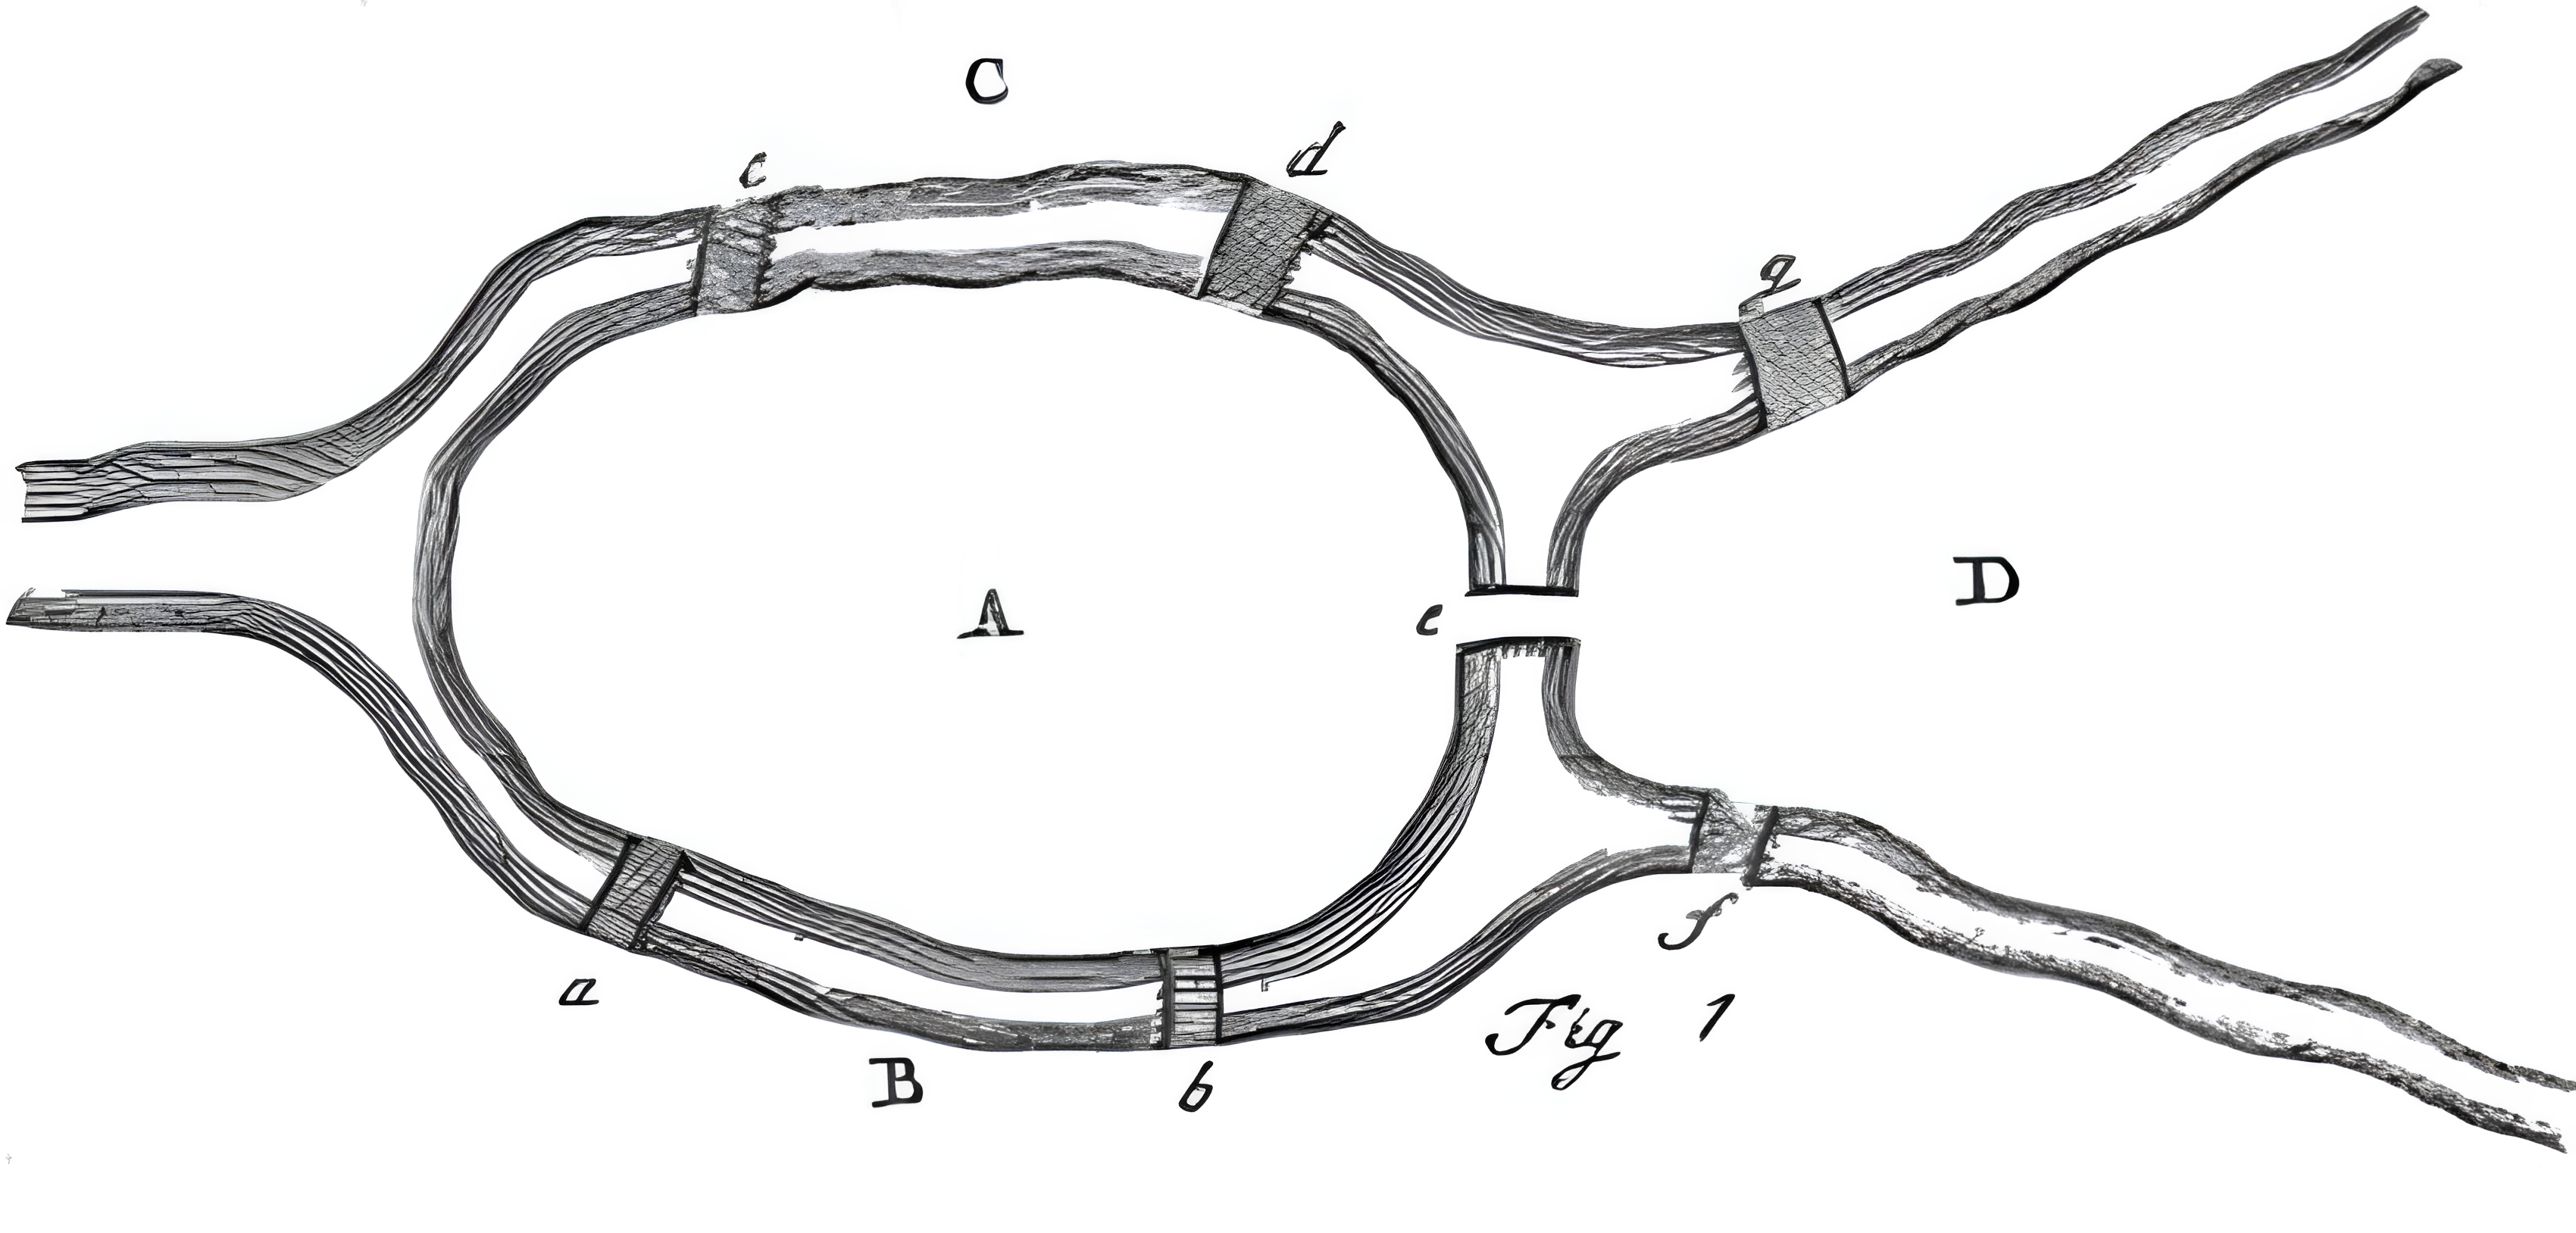
\includegraphics[width=0.4\textwidth]{pictures/SevenBridges.png}
\caption{Illustration du problème des sept ponts de Königsberg}
\label{img:seven-bridges}
\end{figure}

Au cours du XIX\textsuperscript{e} siècle, certains grands mathématiciens ont eu l’occasion de poser une pierre à l’édifice de ce qu’est l’actuelle topologie. Bernhard Riemann a travaillé sur la géométrie complexe, dont certains résultats sont très liés à notre domaine. Enrico Betti a, quant à lui, étudié la notion de connexité. Cela lui a permis de donner son nom à un invariant topologique : les nombres de Betti. Felix Klein a été à l’initiative du programme d’Erlangen. Ce dernier a pour but d’étudier la géométrie, et en particulier les différentes géométries, d’un point de vue global. C’est ainsi qu’ont été introduites les notions d’actions de groupe et d’invariants topologiques.

C’est en 1895 que la topologie algébrique commence à ressembler à ce que nous connaissons, notamment avec les travaux d’Henri Poincaré et son livre \textit{Analysis Situs}. C’est en grande partie à lui que l’on doit les résultats sur lesquels nous allons nous intéresser dans ce rapport, tels que le groupe fondamental. Par exemple, il s’est posé la question suivante : les nombres de Betti peuvent-ils représenter une surface, topologiquement parlant ? Nous reconnaissons ici les premiers questionnements sur les invariants topologiques.

Ce dernier mathématicien n’a malheureusement pas découvert tout le potentiel algébrique existant derrière les invariants topologiques qu’il a étudiés, et notamment les nombres de Betti. Cette découverte, de laquelle découleront les groupes d’homologie, a été initiée par Emmy Noether en 1926. C’est également à elle que nous devons le formalisme actuel de l’algèbre, de la topologie ainsi que de la topologie algébrique.

\subsubsection{Contexte et objectifs}

Dans la branche des mathématiques fondamentales, nous cherchons à établir des théorèmes de classification, ou autrement dit des relations d’équivalence sur un ensemble d’objets. Nous pouvons prendre l’exemple des espaces vectoriels finis, qui sont classifiés à isomorphisme près par leur dimension.

C’est dans le même espoir que la topologie algébrique se caractérise : l’objectif est de classifier les espaces topologiques homéomorphes les uns aux autres. Il a cependant été démontré \cite{homeoImpossible} qu’il est impossible d’effectuer un tel résultat. Alors, la topologie algébrique se retrouve en quête d’outils permettant une classification de ces espaces, prenant en compte les invariants topologiques.

\bigskip Ce mémoire, issu de trois mois de recherche et de lecture, est décomposé en deux grands chapitres, chacun centré sur un invariant topologique. Historiquement, ils ont été introduits comme étant une potentielle solution à notre problème de classification, mais nous savons de nos jours qu'ils ne suffisent pas.

Plus précisément, le premier chapitre sert d'introduction, où l'on expose le contexte et les notions préliminaires nécessaires pour la compréhension de la suite. Le second chapitre se concentre sur le \emph{groupe fondamental}, un outil puissant mais dont l'utilisation reste complexe. Bien que celui-ci offre une visualisation assez évidente, la théorie est tout autre, notamment à cause des notions complexes nécessaires à y introduire. Le groupe fondamental du cercle, dont l'étude recouvre plusieurs pages de résultats et de preuves, en est un parfait exemple. Le troisième chapitre se focalise sur les \emph{groupes d'homologies}, un outil qui vient aux antipodes du groupe fondamental. Leur usage sont bien plus efficaces, preuves à l'appui, et permettent d'étudier des espaces plus complexes. Néanmoins, l'intuition est ici limitée, notamment car la représentation visuelle de l'outil ne se fait que peu (voire pas). Ce chapitre est découpé en trois sections, chacune étant centrée sur une homologie en particulier. Ceci permettra de mettre en lumière leurs différences ainsi que leurs points communs : nous verrons en particulier qu'elles sont toutes identiques à isomorphisme près.

Nous retrouverons en annexe deux petits chapitres supplémentaires. Le premier donne des exemples de calculs que nous pouvons effectuer avec l'homologie simpliciale (voir chapitre \ref{chp:homology}). Le second est une brève introduction à la théorie des catégories, une branche des mathématiques sur laquelle se fonde la topologie algébrique (d'où l'utilisation des flèches).
\section{Notations}
Pour une question de lisibilité et de clarté, nous avons choisi d'utiliser des notations classiques de topologie algébrique.
\begin{itemize}
    \item $\bb{Z}$ : le groupe des entiers relatifs, muni de l'addition ;
    \item $\bb{Z}_n$ : le groupe des entiers modulo $n$ (aussi noté $\bb{Z}/n\bb{Z}$) ;
    \item $\bb{R}^n$ : l'espace euclidien de dimension $n$ ;
    \item $D^n$ : le disque unité dans $\bb{R}^n$, l'ensemble de tous les vecteurs de longueur inférieure ou égale à~1 ;
    \item $\s{n}$ : la sphère unité dans $\bb{R}^{n+1}$, l'ensemble de tous les vecteurs de longueur 1 ;
    \item $\mathcal{V}(x)$ : l'ensemble des voisinages du point $x$ ;
    \item $\cong$ : la relation d'isomorphisme  ;
    \item $\simeq$ : l'équivalence d'homotopie ;
    \item $\sim$ : l'équivalence d'homologie ;
    \item $\approx$ : sauf mention contraire, pour une relation d'équivalence ;
    \item Pour deux applications $f,g$ telles que $dom(f)=cod(g)$, nous noterons $fg$ la composition de $f$ et $g$, habituellement notée $f\circ g$.
\end{itemize}

Sauf mention contraire, toutes les applications considérées seront supposées continues. Également, les espaces considérés seront supposés muni d'une topologie.
\section{Préliminaires}

Nous supposerons ici que les notions de licence sur l'algèbre et la topologie sont acquises. Néanmoins, certains rappels sont effectués sur des notions essentielles pour le mémoire. Nous retrouverons également des notions complémentaires comme celles sur les homotopies.

\subsection{Topologie}
\subsubsection{Espace topologique}

\begin{definition}
On appelle \emph{espace topologique} un couple $(X,\mathcal{T})$, où $X$ est un ensemble et $\mathcal{T}$ une famille de parties de $X$, appelées \emph{ouverts} de $X$, vérifiant : \begin{enumerate}
    \item Les ensembles $\emptyset$ et $X$ sont des ouverts ;
    \item Toute réunion d'ouverts est un ouvert ;
    \item Une intersection finie d'ouverts est un ouvert.
\end{enumerate}
Les complémentaires des éléments de $\mathcal{T}$ sont appelés les \emph{fermés} de $E$.
\end{definition}

\begin{definition}
Un espace topologique $X$ est dit \emph{Hausdroff}, ou séparable, si pour tout couple d'éléments distincts $(x,y)\in X^2$, il existe $U\in\vois(x)$ et~$V\in~\vois(y)$, tel que $U\cap V=\emptyset$.
\end{definition}

Sauf mention contraire, nous désignerons tout au long du mémoire par $X$ un espace topologique, que nous appelons par abus de langage simplement espace.

\subsubsection{Connexité}

Intuitivement, un espace est dit connexe lorsqu'il est constituer d'un seul "morceau".

\begin{definition}
Un espace $X$ est dit \emph{connexe} s'il vérifie l'une des quatres propositions équivalentes : \begin{enumerate}
    \item L'espace n'est pas la réunion de deux ouverts non vides disjoints.
    \item L'espace n'est pas la réunion de deux fermés non vides disjoints.
    \item Les seuls éléments à la fois ouverts et fermés sont $\emptyset$ et $X$.
    \item Toute application continue de $X$ dans $\{0,1\}$ muni de la topologie discrète est constante.
\end{enumerate}

Pour un espace $X$, on appelle \emph{composante connexe} de $x$ dans $X$ la réunion de toutes les parties connexes contenant $x$. C'est la plus grande partie connexe contenant ce point, au sens de l'inclusion. L'ensemble des composantes connexes de $X$ forment une partition de l'espace $X$.

On dit que deux points sont \emph{connectés} s'ils appartiennent à la même composante connexe.
\end{definition}

En pratique, nous préférons utiliser une notions de connexité plus forte, qui est la connexité par arc.

\begin{definition}\label{def:path}
On appelle \emph{chemin} entre deux points $x_0$ et $x_1$ de $X$ une application $\gamma:[0,1]\to X$ continue, et telle que~$\gamma(0)=x_0$ et~$\gamma(1)=x_1$.
\end{definition}

\begin{remark}
Il est important de noter que les chemins ont une direction, donnée par l'application associée (de~$\gamma(0)$ vers $\gamma(1)$).
\end{remark}

\begin{exemple}
Sur l'espace euclidien $\bb{R}^n$, tout couple de point possède un chemin linéaire. Pour $x,y\in\bb{R}^n$, ce chemin est donné par l'application $t\mapsto (1-t)x+ty$.
\end{exemple}

\begin{definition}
Un espace $X$ est dit \emph{connexe par arc} si pour tout couples de points il existe un chemin reliant ces deux points.
\end{definition}

Nous verrons que les espaces connexes par arc sont connexes, mais l'exemple suivant nous montre que la réciproque n'est pas vraie.

\begin{exemple}
On considère le graphe de l'application $x\mapsto\sin\left(\frac{1}{x}\right)$ pour $x\in]0,1]$, auquel on ajoute son adhérence~$\{0\}\times[-1,1]$. Cet espace est connexe, mais nous ne pouvons pas créer de chemin entre un point du graphe et un point de l'adhérence. L'espace est alors non connexe par arc.
\begin{figure}[h]
    \centering
\begin{tikzpicture}
  \begin{axis}[
      axis lines=middle,
      xlabel={$x$},
      ylabel={$y$},
      domain=0.001:1, % éviter x=0
      samples=1000,
      xmin=-0.1, xmax=1.1,
      ymin=-1.2, ymax=1.2,
      width=10cm, height=6cm,
      xtick={0,0.5,1},
      ytick={-1,0,1},
      axis line style={->},
      smooth,
  ]
    % Courbe y = sin(1/x)
    \addplot[blue, thick] {sin(deg(1/x))};

    % Segment rouge de (0,-1) à (0,1)
    \addplot[red, very thick] coordinates {(0,-1) (0,1)};
  \end{axis}
\end{tikzpicture}
\label{tkz:non-path-connected}
\caption{Graphe de la courbe $x\mapsto\sin\left(\frac{1}{x}\right)$ (bleu) et son adhérence (rouge), connexe mais pas par arc}
\end{figure}
\end{exemple}

%\begin{exemple}
%Dans l'exemple qui suit la définition \ref{def:path}, nous avons vu qu'il existe un chemin pour tout couple de points de $\bb{R}^n$. On peut alors dire que l'espace euclidien $\bb{R}^n$ est connexe par arc.
%\end{exemple}

\begin{theorem}
Un espace connexe par arc est connexe.
\end{theorem}
La preuve de ce théorème se déroule par l'absurde, en supposant que l'espace est non connexe. L'idée est alors de définir l'espace comme deux ouverts disjoints non vides., et de considérer un chemin continue entre un point d'un ouvert vers l'autre. La contradiction découle du fait que $[0,1]$ n'est pas l'union de deux ouverts disjoints.

\subsubsection{Comparaisons d'espaces}

Il existe plusieurs moyens de comparer les espaces par des relations d'équivalences. Nous commençons par la relation la plus forte entre espaces : l'homéomorphisme.

\begin{definition}\label{def:homeo}
Un \emph{homéomorphisme} entre deux espaces $X$ et $Y$ est une application continue, inversible, et d'inverse continue. S'il existe un homéomorphisme entre $X$ et $Y$, on dit alors qu'ils sont \emph{homéomorphes}.
\end{definition}

\begin{exemple}
Le cercle $\s{1}$ auquel on supprime un point est homéomorphe à $\bb{R}$. De manière générale, la sphère~$\s{n}$ sur laquelle on supprime un point est homéomorphe à $\bb{R}^n$.

Le cercle est le carré sont homéomorphes. Intuitivement, il suffit soit d'arrondir les côtés du carré, soit de "pincer" quatres points du cercle.
\end{exemple}

La seconde relation est à propos de l'homotopie. Moins puissante que l'homéomorphisme, elle conserve toutefois la continuité dans l'espace ainsi que la connexité.

\begin{definition}\label{def:homotopy-spaces}
Deux applications $f_0,f_1:X\to Y$ sont dites \emph{homotopes} s'il existe une application continue~$F:X\times [0,1]\to Y$ telle que $F(0,x)=~f_0(x)$ et~$F(1,x)=f_1(x)$. Intuitivement, cela signifie qu'il existe une famille d'application~$f_t$, continue en $t$, permettant de passer de $f_0$ à $f_1$.
\end{definition}

De cette définition découle un cas particulier, lorsque le premier espace se rétracte en le second.

\begin{definition}\label{def:retracts}
Une \emph{déformation par rétraction} d'un espace $X$ en un sous-espace $A$ est une homotopie entre $f_0=id_X$, et $f_1(X)=A$, qui vérifie $f_t|_A=id_A$ pour tout $t\in[0,1]$. Nous appelons dans ce cas l'application $f_1$ une \emph{rétraction}.
\end{definition}

\begin{exemple}
Le disque $D^{n}$ se déforme par rétraction en un point.

\begin{figure}[H]
    \centering
    \begin{tikzpicture}
    \filldraw[lightgray] (0,0) circle(1cm);
    \filldraw[] (0,0) circle(1pt); %node[below right]{};
    \draw[thick] (0,0) circle(1cm);
    \draw[->, >=stealth] (1,0) -- (0.1, 0);
    \draw[->, >=stealth] (-1,0) -- (-0.1, 0);
    \draw[->, >=stealth] (0,1) -- (0,0.1);
    \draw[->, >=stealth] (0,-1) -- (0, -0.1);
    \draw[->, >=stealth] (1.4142135624/2,1.4142135624/2) -- (0.1, 0.1);
    \draw[->, >=stealth] (-1.4142135624/2,1.4142135624/2) -- (-0.1, 0.1);
    \draw[->, >=stealth] (1.4142135624/2,-1.4142135624/2) -- (0.1, -0.1);
    \draw[->, >=stealth] (-1.4142135624/2,-1.4142135624/2) -- (-0.1, -0.1);
    \end{tikzpicture}
    \caption{Rétraction par déformation du disque $D^2$ vers le point}
    \label{fig:def-retract-disk}
\end{figure}
\end{exemple}

\begin{definition}\label{def:homotopy-equiv}
Une application $f:X\to Y$ est une \emph{équivalence d'homotopie} s'il existe $g:Y\to X$ tel que~$fg\simeq id_Y$ et $gf\simeq id_X$. Dans ce cas, nous disons que $X$ et $Y$ sont homotopiquement équivalents, que l'on note $X\simeq Y$.
\end{definition}

\begin{exemple}
Pour une déformation par rétraction de $X$ vers $A$, avec $i:A\to X$ l'inclusion et $r:X\to A$ la rétraction, nous avons $ri\simeq id_A$ et $ir\simeq id_X$.
\end{exemple}

\subsection{Algèbre}

Sauf mention contraire, nous désignerons par $G$ un groupe, et $H$ un sous-groupe de $G$.

\subsubsection{Quotient}

\begin{definition}
On dit que le sous-groupe $H$ de $G$ est \emph{normal} s'il est stable par automorphisme intérieur, c'est à dire vérifiant pour tout $g\in G$ l'inclusion $gHg\inv\subset H$.
\end{definition}

Les sous-groupes normaux sont intéressants car permettent de pratiquer le quotient. Si un sous-groupe n'est pas normal pour un groupe, il peut l'être pour un sous-groupe.

\begin{definition}\label{def:normalizer}
Nous disons d'un élément $g$ qu'il \emph{normalise} $H$ s'il vérifie $gHg\inv=H$. L'ensemble des éléments qui normalisent~$H$ est appelé \emph{normalisateur} de $H$, noté~$N(H)$. Le normalisateur est le plus petit sous-groupe normal contenant $H$, donc $H\subset N(H)$.
\end{definition}

\subsubsection{Abélianisation}

Il arrive que le groupe que nous étudions ne soit pas commutatif. Dans ce cas, nous pouvons nous intéresser à son plus grand sous-groupe abélien.

\begin{definition}
Soient $g,h\in G$. On appelle \emph{commutateur} de $g$ et $h$ l'élément~$[g,h]=ghg\inv h\inv$. Le groupe généré par l'ensemble des commutateurs de $G$ est appelé \emph{groupe dérivé} et noté $[G,G]$, c'est le plus petit sous groupe normal tel que le quotient $G/[G,G]$ soit abélien. Ce dernier est appelé \emph{abélianisé} de $G$.
\end{definition}

\subsubsection{Premier théorème d'isomorphisme}

\begin{theorem}[Premier théorème d'isomorphisme]
Soient $G$ et $G'$ deux groupes, et soit un morphisme de groupes $f:G\to G'$. Il existe une unique application $\overline{f}:G/\ker(f)\to \im(f)$, qui à~$\alpha\in G/\ker(f)$ associe~$f(x)$, où $x$ est un représentant de la classe $\alpha$.

L'application $\overline{f}$ est un isomorphisme entre $G/\ker(f)$ et le groupe $\im(f)$. En notant $i:\im(f)\to~G'$ l'injection canonique et $\pi:G\to~\ker(f)$ la surjection canonique, nous avons le diagramme suivant commutatif :
\begin{figure}[H]
    \centering
    \begin{tikzcd}
      G \arrow[d, twoheadrightarrow, "\pi"] \arrow[r, "f"] & G'\\
      G/\ker(f) \arrow[r, "\overline{f}"] & \im(f) \arrow[u, hookrightarrow, "i"]
\end{tikzcd}
\end{figure}
\end{theorem}

Les diagrammes commutatifs sont aussi omniprésents en algèbre homologique, comme nous le verrons durant le chapitre \ref{chp:homology}.

\subsection{Algèbre et topologie}

\subsubsection{Propriété universelle quotient}

\begin{definition}
Soit $X$ un espace topologique, muni d'une relation d'équivalence $\sim$. On appelle \emph{topologie quotient} sur $X/\!\sim$, induite par $X$ et $\sim$, la topologie définie par :\[\forall\, U\!\subset\! X/\sim,\qquad U\ ouvert\Leftrightarrow\pi\inv(U)\ ouvert\ dans \ X.\]
\end{definition}

\begin{theorem}[Propriété universelle de l'espace quotient]\label{th:quotient}
Soient $X,Y$ deux espaces topologiques, et soit~$\sim$ une relation d'équivalence sur $X$. Pour $f:X\to Y$ une application continue vérifiant~${x\sim x'\Rightarrow f(x)=f(x')}$, il existe une unique application continue $\overline{f}:X/\!\sim\ \longrightarrow Y$, telle que~$f=\overline{f}\circ \pi$.

De plus, si $f$ vérifie, pour tout $x,x'$ éléments de $X$, $f(x)=f(x')\Rightarrow x\sim x'$, alors $\overline{f}$ est injective.
\end{theorem}

Une preuve de la propriété universelle est donnée en \cite{Homeo-article}.
\chapter{Le groupe fondamental}\label{chp:homotopy}
Nous allons introduire le groupe fondamental, un outil de topologie algébrique, invariant par homéomorphisme. Intuitivement, nous pouvons le voir comme un outil permettant d'étudier le comportement des lacets (voir définition \ref{def:loops}) sur un espace pointé. Cet outil nous permettra de démontrer que la sphère et le tore ne sont pas homéomorphes : l'idée sous-jacente étant que les lacets de la sphère peuvent se contracter en un point (voir figure \ref{fig:lacet-sphere}), tandis que ceux du tore faisant le tour du "trou" en sont incapables (voir figure \ref{fig:lacet-tore}).

\begin{figure}[H]
\centering
\begin{subfigure}[c]{0.6\linewidth}
\centering
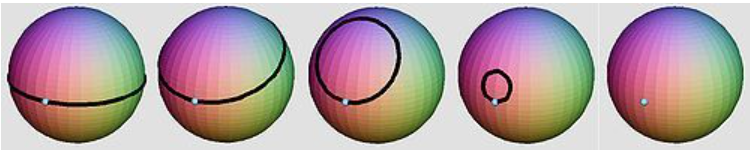
\includegraphics[width=0.7\linewidth]{pictures/sphere-intro.png}
\caption{Lacet de la sphère qui se rétracte}
\label{fig:lacet-sphere}
\end{subfigure}
\begin{subfigure}[c]{0.3\linewidth}
\centering
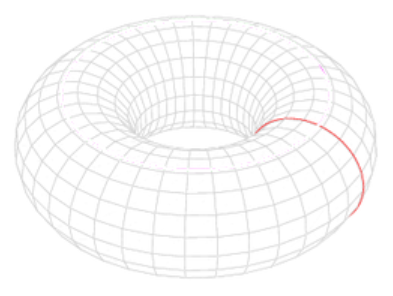
\includegraphics[width=0.7\linewidth]{pictures/tore-intro.png}
\caption{Lacet "coincé" du tore}
\label{fig:lacet-tore}
\end{subfigure}
\end{figure}

Ce chapitre est décomposé en trois grandes sections : \begin{enumerate}
    \item La construction du groupe fondamental, où nous démontrons notamment qu'il possède une structure de groupe (d'où son nom). Nous démontrons ensuite qu'il s'agit d'un invariant par homéomorphisme, et par conséquent qu'il permet de discriminer les espaces. Nous démontrons ainsi que la sphère et le tore ne peuvent être homéomorphes.
    \item Le groupe fondamental du cercle. Sa caractérisation n'est pas si trivial qu'il n'y paraît, et implique notamment l'introduction des revêtements. Suite à ce résultat, nous arrivons à caractériser plusieurs autres groupes fondamentaux.
    \item Les revêtements possèdent un lien encore plus puissant avec les groupes fondamentaux. En particulier, il existe une correspondance de Galois entre les sous-groupes du groupe fondamental et les revêtements de l'espace à isomorphisme près. La démonstration de cette correspondance n'étant pas triviale, elle est découpée en plusieurs parties. 
\end{enumerate}

Sur l'ensemble du chapitre, nous avons semé des exemples simples, apportant une illustration aux propos énoncés.

\section{Un groupe fondamental ?}

Dans cette première section, nous allons définir le groupe fondamental, et démontrer qu'il possède une structure de groupe. Pour cela, nous nous introduisons les lacets, et s'intéresser à eux selon une relation d'équivalence, nommée homotopie.

\begin{definition}\label{def:loops}
Un \emph{lacet}, ou une \emph{boucle}, est un chemin ayant le même point de départ et d'arrivée. Plus formellement, il s'agit d'une application~$\gamma:[0,1]\to X$ telle que~$\gamma(0)=\gamma(1)$. Nous appelons \emph{point de base} le point de départ et d'arrivée du lacet.
\end{definition}

Un lacet est un chemin, il possède donc également une direction, allant de $\gamma(0)$ à $\gamma(1)$.

\begin{exemple}
En considérant le cercle $\s{1}$ dans le plan complexe, le chemin défini par $t\mapsto e^{2i\pi t}$ est un lacet ayant pour point de base~$(1,0)$.
\end{exemple}

L'exemple suivant est important, car introduit le concept de \emph{polygone fondamental}, omniprésent en topologie algébrique, et par conséquent dans ce mémoire. Cette représentation est dite intrinsèque, car ne dépend d'aucun espace environnant. Celle-ci est aux antipodes de leurs plongements dans certains espaces euclidiens~$\bb{R}^n$, même s'il existe un homéomorphisme entre les deux représentations \cite{Homeo-article}.

\begin{exemple}
La figure \ref{tkz:mobius} est la représentation du polygône fondamental du ruban de Mobiüs, un carré avec une identification de deux côtés opposés via une torsion (les deux flèches vont dans deux sens différents).
\begin{figure}[H]
\centering
\begin{subfigure}[b]{0.45\linewidth}
\centering
\begin{tikzpicture}
    % Background color
    \fill[gray!30] (0,0) rectangle (4,4);

    % Top arrow with label A
    \draw[thick, red, ->, >=stealth'] (0,4) -- (4,4) node[midway, below] {\textbf{A}};

    % Bottom arrow with label A
    \draw[thick, red, ->, >=stealth'] (4,0) -- (0,0) node[midway, above] {\textbf{A}};

    % Outer rectangle
    \draw[black, line width=.0mm] (0,0) rectangle (4,4);
\end{tikzpicture}
\caption{Ruban de Mobius}
\label{tkz:mobius}
\end{subfigure}
\begin{subfigure}[b]{0.45\linewidth}
\centering
\begin{tikzpicture}
    % fond gris
    \fill[gray!30] (0,0) rectangle (4,4);
    %flèche du haut
    \draw[thick, red, ->, >=stealth'] (0,4) -- (4,4) node[midway, below] {\textbf{A}};
    %flèche du bas
    \draw[thick, red, ->, >=stealth'] (4,0) -- (0,0) node[midway, above] {\textbf{A}};
    %carré
    \draw[black, line width=.0mm] (0,0) rectangle (4,4);
    
    %gamma'
    \draw[thick, black, ->] (3,0) -- (2.5,1);
    \draw[thick, black] (2.5,1) -- (2,2) node[near start, left] {$\gamma'$};
    \draw[thick, black, ->] (2,2) -- (1.5,3);
    \draw[thick, black] (1.5,3) -- (1,4);

    %gamma
    \draw[thick, ->] (3.4, 2) arc[start angle=0, end angle=360, radius=0.7] node[right] {$\gamma$};
    % Point at (2,2)
    \filldraw[black] (2,2) circle (2pt) node[right] {$x_0$};
\end{tikzpicture}
\caption{Ruban de Mobius et deux lacets}
\label{tkz:mobius-loops}
\end{subfigure}
\end{figure}

Nous pouvons tracer une infinité de lacet sur le ruban, mais deux grandes "familles" en ressortent, illustrés dans la figure \ref{tkz:mobius-loops} : les lacets qui restent dans l'intérieur du carré (comme le lacet $\gamma$), et les lacets qui utilisent l'identification $A$ des côtés (comme le lacet $\gamma'$).
\end{exemple}

\subsection{Homotopie}\label{sec:homotopy}

L'homotopie est la formalisation de l'idée de la déformation d'objets, en particuliers des chemins et lacets sur un espace. Le concept de lacet qui se rétracte (présenté en introduction) devient cohérent d'un point de vue topologique.

\begin{definition}\label{def:homotopy-paths}
Soient $x_0, x_1$ deux points de l'espace $X$, et soient $\gamma_0$ et $\gamma_1$ deux chemins partageant les mêmes extrémités $x_0$ et $x_1$. Une \emph{homotopie} entre $\gamma_0$ et $\gamma_1$ est une application $\Gamma:[0,1]^2\to X$, définie par $\Gamma(t,s)=\gamma_t(s)$, continue en $t$ et telle que, pour tout $t\in[0,1]$, $\gamma_t(0)=x_0$ et $\gamma_t(1)=x_1$.

Intuitivement, cela revient à dire qu'il existe une famille $\gamma_t$ de chemin fixant les extrémités, et continue en $t$. Nous disons alors que $\gamma_0$ est homotope à $\gamma_1$, ou bien que $\gamma_0$ et $\gamma_1$ sont homotopes, et l'on note $\gamma_0\simeq\gamma_1$.
\end{definition}

\begin{figure}[H]
    \centering
    \begin{tikzpicture}
    % Points A et B
    \filldraw[black] (0,0) circle (2pt) node[above left] {$x_0$};
    \filldraw[black] (6,0) circle (2pt) node[above right] {$x_1$};
    % t=0
    \draw[thick, ->, >=stealth] (0,0) .. controls (1.5,0.8) .. (3,1) node[near end, above] {$\gamma_0$}; 
    \draw[thick] (3,1) .. controls (4.5,0.8) .. (6,0);
    %t=.25
    \draw[dashed, ->, >=stealth'] (0,0) .. controls (1.5,0.4) .. (3,0.5); 
    \draw[dashed] (3,0.5) .. controls (4.5,0.4) .. (6,0);
    %t=0.5
    \draw[thick, dashed, ->, >=stealth'] (0,0) -- (3,0)  node[near end, above] {$\gamma_{\frac{1}{2}}$}; 
    \draw[thick, dashed] (3,0) -- (6,0);
    %t=.75
    \draw[dashed, ->, >=stealth'] (0,0) .. controls (1.5,-0.4) .. (3,-0.5); 
    \draw[dashed] (3,-0.5) .. controls (4.5,-0.4) .. (6,0);
    % t=1
    \draw[thick, ->, >=stealth'] (0,0) .. controls (1.5,-0.8) .. (3,-1) node[near end, below] {$\gamma_1$}; 
    \draw[thick] (3,-1) .. controls (4.5,-0.8) .. (6,0);
\end{tikzpicture}
    \caption{Homotopie entre les chemins $\gamma_0$ et $\gamma_1$}
    \label{tkz:path-homotopy}
\end{figure}

\begin{exemple}
Dans l'espace euclidien $\bb{R}^n$, il existe toujours une homotopie linéaire entre deux chemins avec les mêmes extrémités. En effet, en notant $\gamma_0$ et $\gamma_1$ deux chemins d'extrémités communes $x_0$ et $x_1$, nous avons l'homotopie suivante, pour~$t\in[0,1]$ :  $\gamma_t(s)=(1-t)\gamma_0(s)+t\gamma_1(s)$. Il est facile de vérifier que $\gamma_t(0)=x_0$ et~$\gamma_t(1)=x_1$, pour tout $t\in[0,1]$.
\end{exemple}

Plutôt que de s'intéresser à l'ensemble des lacets, nous allons préférer les étudier à homotopie près. D'une part, il est possible dans certains cas de passer d'une infinité de lacets à un nombre fini de classes d'équivalences. Et d'autre part, les classes d'homotopie de lacets possèdent une structure naturelle de groupe. C'est ce que nous allons montrer par la suite.

\begin{proposition}
La relation d'homotopie entre chemins est une relation d'équivalence. Nous noterons $[\gamma]$ la classe d'équivalence de $\gamma$ sous la relation d'homotopie, et nous appellée \emph{classe d'homotopie} de $\gamma$.
\end{proposition}

En rappellant qu'une relation d'équivalence est définie comme étant réflexive, symétrique et associative, la démonstration consiste simplement à montrer successivement que les trois propriétés sont vérifiées par la relation d'homotopie.
\begin{proof}
\textit{(Réfléxivité)} Pour tout chemin $\gamma$ sur $X$, il existe l'homotopie constante $\gamma_t(s)=\gamma(s)$. Nous en conluons que $\gamma\simeq\gamma$.

\textit{(Symétrie)} Pour toute homotopie $\gamma_t(s)$ entre $\gamma$ et$\gamma'$, il est clair que l'homotopie $\gamma_{1-t}$ permet d'aller de~$\gamma'$ vers $\gamma$. Nous en concluons que $\gamma'\simeq\gamma$.

\textit{(Associativité)} Soient $\gamma\simeq\gamma'$ et $\gamma'\simeq\gamma''$. En notant $\gamma_t$ l'homotopie entre $\gamma$ et $\gamma'$ et $\gamma_t'$ l'homotopie entre $\gamma'$ et~$\gamma''$, nous pouvons  construire l'homotopie $\gamma''_t$ entre $\gamma$ et $\gamma''$, correspondant aux deux homotopies l'une après l'autre : \[\gamma''_t(s)= \left\{\begin{matrix}
\gamma_{2t}(s),&\text{si }t\in[0,\frac{1}{2}], \\
\gamma'_{2t-1}(s),&\text{si }t\in[\frac{1}{2},1].
\end{matrix}\right.\]Celle-ci est continue par définition des deux autres homotopies, en particulier en $1\over 2$ du fait qu'elle se recoupe en le même chemin : $\gamma_1=\gamma'=\gamma'_0$. Nous en concluons que $\gamma\simeq\gamma''$.
\end{proof}

Les lacets étant des chemins, nous pouvons considérer les classes d'homotopie de ceux-ci.

\subsection{Loi de composition interne}

Désormais, pour pouvoir parler de groupe, nous avons besoin d'un opérateur entre les classes d'homotopie. Nous allons alors partir d'une loi de composition interne (LCI) sur les chemins qui soit compatible avec la relation d'équivalence d'homotopie.

\begin{wrapfigure}{r}{0.3\textwidth}
    \centering
    \begin{tikzpicture}
    \filldraw[black] (0,0) circle (2pt) node[above left] {$x_0$};
    \filldraw[black] (2,0.5) circle (2pt) node[above] {$x_1$};
    \filldraw[black] (3,1.7) circle (2pt) node[above left] {$x_2$};
    \draw[thick, ->, >=stealth, red] (0,0) .. controls (0.5,0) .. (1,0.05) node[near start, above] {$\gamma$}; 
    \draw[thick, red] (1,0.05) .. controls (1.5,0.2) .. (2,0.5) ; 
    \draw[thick, blue, ->, >=stealth'] (2,0.5) .. controls (2.5,0.6) .. (3,1) ; 
    \draw[thick, blue] (3,1) .. controls (3.1,1.2) .. (3,1.7) node[near end, right] {$\gamma'$};
    \node[violet] at (2,0.2) {$\gamma\cdot\gamma'$};
    \end{tikzpicture}
\end{wrapfigure}

\phantom{}
\begin{definition}
Pour $\gamma,\gamma'$ deux chemins sur un espace $X$ tels que~$\gamma(1)=\gamma'(0)$, nous pouvons définir le lacet $\gamma\cdot\gamma'$ comme étant le chemin résultat de la \emph{concaténation} de $\gamma$ et $\gamma'$. Formellement, nous le définissons comme suit : \[\gamma\cdot \gamma'(s)=\left\{\begin{matrix}
\gamma(2s)&\text{si }0\leq s\leq \frac{1}{2}\\ 
\gamma'(2s-1)&\text{si }\frac{1}{2}\leq s\leq 1.
\end{matrix}\right.\]

En particulier pour les lacets avec le même point de base, la concaténation est une LCI.
\end{definition}

%En effet, la concaténation de deux lacets donne un lacet qui passera sur le point de base à mi-parcours. Nous pouvons visualler cela avec le chiffre 8, qui est concaténation d'un lacet supérieur et un lacet inférieur, où le point de base est le point d'intersection des deux lacets.

\begin{proposition}
La LCI de la concaténation de lacets est compatible avec la relation d'homotopie. Nous définissons ainsi une LCI sur les classes d'homotopie de lacets, telle que pour $\gamma$ et $\gamma'$ deux lacets ayant le même point de base, on ait $[\gamma][\gamma']=[\gamma\cdot\gamma']$.
\end{proposition}

%La démonstration consiste à vérifier si, pour deux paires de lacets homotopes, la concaténation d'éléments de chaque pair est homotope à la concaténation des deux autres. Pour cela, nous allons construire l'homotopie entre les deux concaténations, à partir des homotopies de base.

Nous utiliserons le terme de concaténations lorsqu'il s'agit de lacets, et de produit lorsqu'il s'agit de classes.


\begin{proof}
Soient $\gamma\simeq\gamma'$ et $\zeta\simeq\zeta'$ quatres lacets ayant un même point de base $x_0\in X$. Il nous suffira de montrer que $\gamma\cdot\zeta\simeq\gamma'\cdot\zeta'$.

Notons respectivement $\gamma_t$ et $\zeta_t$ les homotopies allant de $\gamma$ vers $\gamma'$ et de $\zeta$ vers~$\zeta'$, et considérons l'application obtenue par concaténation de ces homotopies : \begin{equation}\label{eq:homotopy-concatenate}
\tau_t(s)=\gamma_t\cdot\zeta_t(s)=\left\{\begin{matrix}
\gamma_t(2s)&\text{si }0\leq s\leq \frac{1}{2}\\ 
\zeta_t(2s-1)&\text{si }\frac{1}{2}\leq s\leq 1.
\end{matrix}\right.
\end{equation}

Montrons que $\tau_t$ est une homotopie entre $\gamma\cdot\zeta$ et $\gamma'\cdot\zeta'$. D'une part, les points de départs et d'arrivées sont respectivement $\tau_0=\gamma_0\cdot\zeta_0=\gamma\cdot\zeta$, et $\tau_1=\gamma_1\cdot\zeta_1=\gamma'\cdot\zeta'$. Pour ce qui est des extrémités des lacets, ceux-ci restent constant en $x_0$ par définition de $\gamma_t$ et $\zeta_t$ : $\gamma_t\cdot\zeta_t(0)=\gamma_t(0)=x_0$ et $\gamma_t\cdot\zeta_t(1)=\zeta_t(1)=x_0$. Enfin la continuité de $\tau_t$ est évidement due à celle des deux autres homotopies.

Nous venons de prouver qu'il existe une homotopie entre $\gamma\cdot\zeta$ et $\gamma'\cdot\zeta'$, ce qui les rend homotopes.
\end{proof}

\begin{definition}
L'ensemble des classes d'homotopie de lacets de $X$ basés en $x_0\in X$ est appelé le \emph{groupe fondamental} de $X$ en $x_0$, ou sur l'espace pointé $(X,x_0)$, et on note $\pi_1(X,x_0)$.
\end{definition}

Notre objectif est de démontrer que le groupe fondamental muni du produit sur les classes de lacets possède une structure de groupe. Nous commençons par démontrer qu'il existe un élément neutre.

\begin{lemma}
L'élément neutre pour le produit de classes de lacets est la classe du lacet constant $c$ en le point de base.
\end{lemma}

Notre démonstration sera constructive : nous expliciterons les homotopies entre les lacets. A notre connaissance, il n'existe pas de démonstration entrant autant dans les détails, pour la simple raison de la trivialité du raisonnement.

\begin{proof}
Soit~${\alpha\in\pi_1(X,x_0)}$ une classe d'homotopie, avec $\gamma$ un représentant. Nous construirons deux homotopies : l'une entre $\gamma\cdot c$ et $\gamma$, et l'autre entre $c\cdot\gamma$ et $\gamma$. Cela permet de déduire que $\alpha\cdot [c]\simeq\alpha$ et~$[c]\cdot \alpha\simeq \alpha$, et donc démontrer que $[c]$ est le neutre pour le produit.

On construit tout d'abord l'application permettant d'"effacer" homotopiquement le lacet constant à $\gamma\cdot c$ : \[t\in[0,1]\mapsto\gamma_t(s)=\left\{\begin{matrix}
\gamma\big(2s-t\big)&\text{si }0\leq s\leq \frac{1}{2}(1+t)\\ 
c(0)=x_0&\text{sinon}.
\end{matrix}\right.\]

L'application est continue en $s$, en particulier pour $s=\frac{1}{2}(1+t)$, du fait que $\gamma(2s-t)=\gamma(1)=x_0$. L'application est continue en $t$, et les extrémités sont clairement conservées. Il s'agit alors d'une homotopie entre $\gamma_0=\gamma\cdot c$ et $\gamma_1=\gamma$.

De manière similaire, nous pouvons construire l'application permettant d'effacer homotopiquement le lacet constant à $c\cdot\gamma$ : \[t\in[0,1]\mapsto\gamma'_t(s)=\left\{\begin{matrix}
c\left(0\right)=x_0&\text{si }0\leq s\leq \frac{1}{2}(1-t)\\ 
\gamma\left(\frac{2s+t-1}{t+1}\right)&\text{si }\frac{1}{2}(1-t)\leq s\leq 1.
\end{matrix}\right.\]

Montrons qu'il s'agit d'une homotopie, en commençant par la continuité. Pour $s=\frac{1}{2}(1-t)$, on a ${2s+t-1=(1-t)+t-1=0}$, d'où $\gamma\big(\frac{2s+t-1}{t+1}\big)=x_0$. Cela montre que notre application est continue. De même que précédemment, il est facile de vérifier que cela constitue une homotopie entre les lacets~$c\cdot\gamma$ et $\gamma$.

Nous en concluons que la classe d'homotopie $[c]$ est l'élément neutre pour le produit de classes.
\end{proof}

Nous allons désormais démontrer que la structure du groupe fondamental justifie une telle terminologie.

\begin{theorem}
L'ensemble $\pi_1(X,x_0)$ muni du produit sur les classes de lacets possède une structure de groupe, avec le lacet constant comme élément neutre.
\end{theorem}

Nous allons démontrer ce résultat de manière classique, en prouvant l'existance de l'inverse, et en prouvant l'associativité. Encore une fois, cette preuve est constructive, et ne se fait que rarement (voire jamais).

\begin{proof}
On considère le groupe fondamental $\pi_1(X,x_0)$ pour un espace $X$ et un point $x_0\in X$. Nous avons déjà démontré dans le lemme précédent que le lacet constant est l'élément neutre.

\bigskip \textit{(Inverse)} Soit $\alpha\in\pi_1(X,x_0)$ et soit $\gamma$ un lacet représentant de la classe. Notons $\overline{\gamma}(s)=\gamma(1-s)$ le lacet inverse de $\gamma$. Nous allons montrer que $\gamma\cdot\overline{\gamma}\simeq c$ et $\overline{\gamma}\cdot\gamma\simeq c$, ce qui suffit pour démontrer l'existance de l'inverse : $\alpha\cdot [\overline{\gamma}]=[c]$ et $[\overline{\gamma}]\cdot \alpha=[c]$.

Pour cela, on considère une première application, dans le but de vérifier $\gamma\cdot \overline{\gamma}\simeq c$ : \[t\in[0,1]\mapsto\gamma_t(s)=\left\{\begin{matrix}
\gamma\big(2s(1-t)\big)&\text{si }0\leq s\leq \frac{1}{2}\\ 
\overline{\gamma}\big((2s-1)(1-t)+t\big)&\text{si }\frac{1}{2}\leq s\leq 1.
\end{matrix}\right.\]Montrons qu'il s'agit d'une homotopie, en commençant par la continuité. La consitnuité en $t$ est évidente car n'agit seulement de chemin linéaire sur $[0,1]$. La continuité en $s$ est de même simple, mais vérifions la jonction en $1\over2$ : d'un côté, nous avons $\gamma(2s(1-t))=\gamma(1-t)$, et de l'autre $\overline{\gamma}((2s-1)(1-t)+t)=\overline{\gamma}(t)=\gamma(1-t)$. Aux extrémités de $s$, nous avons $\gamma_t(0)=\gamma(0)=x_0$, et $\gamma_t(1)=\overline{\gamma}(1-t+t)=\gamma(0)=x_0$. Il s'agit finalement d'une homotopie entre $\gamma_0=\gamma\cdot \overline{\gamma}$ et $\gamma_1=\gamma(0)\cdot\overline{\gamma}(0)=c$  Ensuite, il est facile de vérifier la continuité en $t$, et que l'on a $\gamma_0=\gamma\cdot\overline{\gamma}$ et $\gamma_1=c$. Nous pouvons alors en déduire que cette application est une homotopie entre les lacets $\gamma\cdot\overline{\gamma}$ et $c$.

\bigskip \textit{(Associativité)} Il nous reste à démontrer l'associativité. Soient $\alpha,\beta,\delta\in\pi_1(X,x_0)$, avec comme représentants respectifs~$\gamma,\zeta,\theta$. Il nous suffira de  montrer que l'on a~$\gamma\cdot(\zeta\cdot\theta)\simeq(\gamma\cdot\zeta)\cdot\theta$. Nous commençons par écrire explicitement la définition de ces lacets : \[\begin{split}
\gamma\cdot(\zeta\cdot\theta)(s)&=\left\{\begin{matrix}
    \gamma(2s)&\text{si }0\leq s\leq\frac{1}{2}\\
    \zeta\cdot\theta(2s-1)&\text{si }\frac{1}{2}\leq s\leq 1
\end{matrix}\right.\\
&=\left\{\begin{matrix}
    \gamma(2s)&\text{si }0\leq s\leq\frac{1}{2}\\
    \zeta(4s-2)&\text{si }\frac{1}{2}\leq s\leq\frac{3}{4}\\
    \theta(4s-3)&\text{si }\frac{3}{4}\leq s\leq1,
\end{matrix}\right.
\end{split}\]et\[\begin{split}
(\gamma\cdot\zeta)\cdot\theta(s)&=\left\{\begin{matrix}
    \gamma\cdot\zeta(2s)&\text{si }0\leq s\leq\frac{1}{2}\\
    \theta(2s-1)&\text{si }\frac{1}{2}\leq s\leq 1
\end{matrix}\right.\\
&=\left\{\begin{matrix}
    \gamma(4s)&\text{si }0\leq s\leq\frac{1}{4}\\
    \zeta(4s-1)&\text{si }\frac{1}{4}\leq s\leq\frac{1}{2}\\
    \theta(2s-1)&\text{si }\frac{1}{2}\leq s\leq1.
\end{matrix}\right.
\end{split}\]On considère l'application suivante, dans l'objectif d'obtenir une homotopie entre les deux lacets explicités plus haut : \[t\in[0,1]\mapsto h_t(s)=\left\{\begin{matrix}
\gamma\left(\frac{4s}{2-t}\right)&\text{si }0\leq s\leq \frac{1}{4}(2-t)\\
\zeta\left(4s-2+t\right)&\text{si }\frac{1}{4}(2-t)\leq s\leq \frac{1}{4}(3-t)\\
\theta\left(\frac{4s-4}{1+t}+1\right)&\text{si }\frac{1}{4}(3-t)\leq s\leq1.
\end{matrix}\right.\]Montrons désormais qu'il s'agit d'une homotopie. La continuité en $t$ est évidente, et celle en $s$ demande une vérification sur les jonctions. En $\frac{1}{4}(2-t)$, nous avons l'égalité $\gamma\left(\frac{4s}{2-t}\right)=\gamma(1)=x_0$ d'une part, et $\zeta(4s-2+t)=\zeta(0)=x_0$ de l'autre. En $s=\frac{1}{4}(3-t)$, nous avons $\zeta(4s-2+t)=\zeta(1)=x_0$ d'une part et $\theta(\frac{4s-4}{1-t}+1)=\theta(0)=x_0$. De plus pour les extrémités, nous avons $h_t(0)=\gamma(\frac{0}{2-t})=x_0$ et $h_t(1)=\theta(\frac{4-4}{1+t}+1)=\theta(1)=x_0$. Nous pouvons en conclure que $h_t$ définie une homotopie entre $h_0$ et $h_1$, mais quels sotn ces lacets ?Par une simple substitution, nous obtenons les résultats suivants : \[h_0(s)=\left\{\begin{matrix}
\gamma\left(\frac{4s}{2-0}\right)=\gamma\left(2s\right) & 0\leq s\leq \frac{1}{2} \\
\zeta(4s-2+0) & \frac{1}{2}\leq s\leq \frac{3}{4} \\
\theta\left(\frac{4s-4}{1+0}\right)=\theta(4s-3) & \frac{3}{4} \leq s\leq 1,
\end{matrix}\right.\]et \[h_1(s)=\left\{\begin{matrix}
\gamma\left(\frac{4s}{2-1}\right)=\gamma(4s) & 0\leq s\leq \frac{1}{4} \\
\zeta(4s-2+1)=\zeta(4s-1) & \frac{1}{4}\leq s\leq \frac{1}{2} \\
\theta\left(\frac{4s-4}{1+1}\right)=\theta(2s-1) & \frac{1}{2} \leq s\leq 1.
\end{matrix}\right.\]Nous en concluons qu'il s'agit d'une homotopie entre $\gamma\cdot(\zeta\cdot \theta)$ et $(\gamma\cdot \zeta)\cdot \theta$, ce qui permet de démontrer l'associaticité sur le produit des classes d'homotopies.

\bigskip Nous achevons ainsi la démonstration en concluant que le groupe fondamental $\pi_1(X,x_0)$ est un groupe.
\end{proof}

Intuitivement, nous venons de démontrer que les classes d'homotopie ne se préoccupe pas du "temps de parcours" du lacet, seulement du trajet (à homotopie près évidement). Si l'on parcourt un lacet dans un sens puis dans l'autre sens, nous considérons en terme d'homotopie que cela revient à ne pas bouger.

\subsection{Propriétés élémentaires}

Désormais que nous savons qu'il existe une structure de groupe sur un espace, il serait bien de l'utiliser. Avant de voir un exemple concret de calcul de groupe, nous allons voir quelques propriétés de base, en commençant par une définition.

\begin{definition}
Un espace est dit \emph{simplement connexe} si son groupe fondamental est trivial.
\end{definition}

Le terme "simplement" réfère directement à l'ensemble des classes d'homotopies, qui possède un seul élément.

\begin{proposition}
Tout sous-espace convexe $X\subset\bb{R}^n$ est simplement connexe.
\end{proposition}

Nous avons déjà vu dans l'exemple à al suite de la définition \ref{def:homotopy-paths} qu'il existe une homotopie (linéaire) entre tout chemin partageant les mêmes extrémités. Ce résultat reste évidement vraie dans le cas des lacets, ce qui rend l'ensemble des classes réduit à un élément : d'où la proposition !

\begin{proposition}
Soit $X$ un espace, et soient $x_0,x_1\in X$ deux points reliés par un chemin. Les groupes fondamentaux $\pi_1(X,x_0)$ et $\pi_1(X,x_1)$ sont isomorphes.
\end{proposition}



\begin{proof}
Soit $\zeta$ le chemin entre $x_0=\zeta(0)$ et $x_1=\zeta(1)$. Pour un lacet~$\gamma$ de $X$ ayant pour point de base $x_0$, nous avons $\zeta\cdot\gamma\cdot\overline{\zeta}$ qui est un lacet basé en~$x_1$. Nous pouvons alors définir l'application~$\Phi:\pi_1(X,x_0)\to\pi_1(X,x_1)$, qui envoie~$[\gamma]$ sur $[\zeta\cdot\gamma\cdot\overline{\zeta}]$. Montrons que cette application est un morphisme de groupes, puis qu'elle admet un morphisme réciproque, de telle sorte que ce soit un isomorphisme.

Nous devons tout d'abord montrer que l'application est bien définie, c'est à dire pour $\gamma\simeq\gamma'$ deux lacets de $(X,x_0)$, nous avons $\zeta\cdot\gamma\cdot\overline{\zeta}\simeq\zeta\cdot\gamma'\cdot\overline{\zeta}$. En notant~$\gamma_t$ l'homotopie entre $\gamma$ et $\gamma'$, nous avons $\zeta\cdot\gamma_t\cdot\overline{\zeta}$ qui forme une homotopie entre $\zeta\cdot\gamma\cdot\overline{\zeta}$ et $\zeta\cdot\gamma'\cdot\overline{\zeta}$.

\bigskip Soient $\alpha,\alpha'\in\pi_1(X,x_0)$, montrons que $\Phi(\alpha\alpha')=\Phi(\alpha)\Phi(\alpha')$. Soient $\gamma,\gamma'$ deux lacets de $(X,x_0)$, représentants respectifs de $\alpha$ et $\alpha'$. Nous avons : \[\begin{split}
\Phi([\gamma][\gamma'])&=\Phi([\gamma\cdot\gamma'])\\
&=[\zeta\cdot\gamma\cdot\gamma'\cdot\overline{\zeta}]\\
&=[\zeta\cdot\gamma\cdot\overline{\zeta}\cdot\zeta\cdot\gamma'\cdot\overline{\zeta}]\\
&=[\zeta\cdot\gamma\cdot\overline{\zeta}][\zeta\cdot\gamma'\cdot\overline{\zeta}]\\
&=\Phi([\gamma])\Phi([\gamma']).
\end{split}\] Nous pouvons alors en déduire qu'il s'agit d'un morphisme. Désormais, on considère l'application allant de $\pi_1(X,x_1)$ vers $\pi_1(X,x_0)$ par~$\Psi:[\gamma]\mapsto[\overline{\zeta}\cdot\gamma\cdot\zeta]$. Pour la même raison que pour $\Phi$, il s'agit d'un morphisme bien définit. Il est évident que $\Phi$ et $\Psi$ sont des morphismes réciproques l'un par rapport à l'autre, puisque~$[\zeta\cdot\overline{\zeta}]=[c]$ et~$[\overline{\zeta}\cdot\zeta]=[c]$. Nous pouvons en conclure que les deux groupes sont isomorphes.
\end{proof}
\begin{remark}
Autrement dit, le groupe fondamental d'un espace connexe par arc ne dépend pas du point choisi. Nous pouvons alors négliger la notation du point de base pour de tel espace.
\end{remark}

\subsubsection{Morphisme induit}

Le premier résultat qui nous intéresse est celui de l'invariance du groupe fondamental par homéomorphisme. Cela vient du fait de la bonne propriété que possède le groupe fondamental sur les inductions de morphismes :

\begin{definition}
Soit $f:(X,x_0)\to(Y,y_0)$ une application entre deux espaces (le point $x_0$ est envoyé sur $y_0$ via $f$). Le \emph{morphisme de groupes induit} par $f$ se défini par $f_\ast:\pi_1(X,x_0)\to\pi_1(Y,y_0)$, qui à un élément $[\gamma]\in\pi_1(X,x_0)$ renvoie~$[f\gamma]\in\pi_1(Y,y_0)$. 
\end{definition}

En théorie des catégories \ref{chap:categories}, on dit que le groupe fondamental est un \emph{foncteur} entre la catégorie des espaces pointés et la catégorie des groupes. Cela signifie qu'il vérifie le théorème suivant.

\begin{theorem}
Nous avons $id_\ast=id$, et pour $f:Y\to Z, g:X\to Y$,  l'égalité $(fg)_\ast=f_\ast g_\ast$. En théorie des catégories, nous disons que le groupe fondamental est un foncteur \emph{covariant}.
\end{theorem}
\begin{proof}
Le morphisme induit par l'identité $id:X\to X$, est défini par $[\gamma]\mapsto[id(\gamma)]=[\gamma]$, ce n'est rien d'autre que l'identité.

En reprenant les notations de l'énoncé, nous avons l'égalité suivante : \[f_\ast(g_\ast([\gamma]))=f_\ast([g\gamma])=[fg\gamma]=(fg)_\ast([\gamma]).\]
\end{proof}



\begin{theorem}
Soit $X$ et $Y$ deux espaces homéomorphes, et soit $x_0\in X$. L'homéomorphisme~$f:X\to Y$ induit un isomorphisme entre les groupes fondamentaux $f_\ast:\pi_1(X,x_0)\to\pi_1(Y,f(x_0))$.
\end{theorem}
\begin{proof}
Du fait que $f$ soit une bijection, elle admet une inverse. Cette inverse induit une inverse pour $f_\ast$, d'où le fait que les groupes fondamentaux soient isomorphes.
\end{proof}

La contraposée est plus intéressante, puisqu'elle permet d'affirmer grâce au groupe fondamental si deux groupes sont non homéomorphes.

\begin{corollary}
Si deux espaces $X$ et $Y$ ne possèdent pas le même groupe fondamental, alors ils ne sont pas homéomorphes.
\end{corollary}
\begin{remark}
Attention toutefois, la réciproque n'est pas vraie, comme nous pouvons le voir juste après.
\end{remark}

\begin{proposition}\label{prop:eq-homo-same-gr-fund}
Une équivalence d'homotopie $\phi:X\to Y$ induit un isomorphisme  entre$\pi_1(X,x_0)$ et~$\pi_1(Y,\phi(x_0))$, pour tout $x_0\in X$.
\end{proposition}
\begin{proof}

\end{proof}

\begin{proposition}
Si un espace $X$ se rétracte en $A$, alors l'inclusion induit un morphisme injectif~$i_\ast:\pi_1(A,x_0)\to\pi_1(X,x_0)$. Si c'est une déformation par rétraction, alors le morphisme induit est un isomorphisme.
\end{proposition}
\begin{proof}
Soient $r:X\to A$ et $i:A\hookrightarrow X$, tels que nous avons $ri=id_A$, ce qui induit~$r_\ast i_\ast=id$. Du fait qu'avoir un inverse à gauche implique être injectif, on en déduit que $i_\ast$ est un morphisme injectif.

Une déformation par rétraction est un cas particulier d'équivalence d'homotopie, nous pouvons alors utiliser la proposition précédente.
\end{proof}

\begin{comment}
\begin{remark}
Le fait que l'on obtiennent des isomorphismes de groupes fondamentaux sur des espaces non homéomorphes posent problème sur l'efficacité de discrimination du groupe fondamental. Ce n'est pas une méthode efficace pour savoir si deux espaces sont homéomorphes, ou simplement homotopiquement équivalent, ou encore obtenu par déformation par rétraction. Un exemple facile serait le disque qui se rétracte par déformation en un point : les deux espace sont simplement connexes, mais ne sont pas homéomorphes.
\end{remark}
\end{comment}%groupe fonda
\section{Mise en pratique}

Le premier résultat que nous aimerions obtenir est le calcul du groupe fondamental du cercle. Nous verrons que celui-ci est isomorphe à $\bb{Z}$, puisque cela revient à compter le nombre de tour qu'un lacet fait autour du cercle.

Intuitivement, nous devons comprendre que le lacet faisant une fois le tour du cercle (disons le lacet $t\mapsto e^{2i\pi t}$) ne peut se rétracter en le lacet constant. Cela vient du fait que l'on ne peut pas couper le lacet, ni passer au travers le trou à l'intérieur du cercle.

\subsection{Revêtements, première partie}\label{covering-space-intro}

\begin{wrapfigure}{r}{0.2\textwidth}
    \centering
    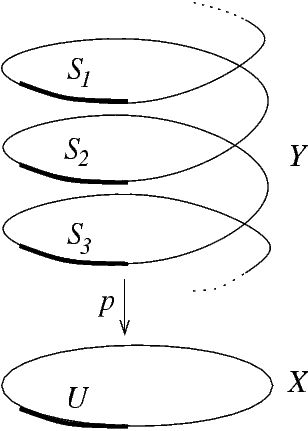
\includegraphics[width=.9\linewidth]{pictures/covering-map-circle.png}
    \caption{\centering Revêtement du cercle}
    \label{fig:cover-circle}
\end{wrapfigure}

Pour comprendre ce qu'est qu'un \emph{revêtement}, nous allons commencer par un exemple classique, celui du cercle.

\begin{exemple}
Nous nous plaçons dans l'espace euclidien en trois dimensions. Notre cercle, ici appelé $X$, se retrouve en dessous d'un autre espace, qui est appelé ici $Y$. La projection $p$ projette $Y$ sur le cercle, ne dépendant pas de la troisième coordonnée.

Le revêtement du cercle $X$ est ici le couple $(Y,p)$. Ce que l'on peut voir sur la figure, est que la préimage ouverte de l'ouvert $U\subset X$ par $p$ est une réunion disjointe d'ouvert $(S_i)_i\subset Y$. On note alors $p\inv=\sqcup_i S_i$. De plus, la projection restreinte à un ouvert $S_i\in p\inv(U)$ nous donne un homéomorphisme avec $U$. Autrement dit, nous avons la projection $p|_{S_i}:S_i\to U$ qui est un homéomorphisme, dit local.

Nous pouvons définir ce revêtement de deux manières différentes. La première est de considérer $Y=\{\big(\cos(2\pi t),\sin(2\pi t), t\big),t\in \bb{R}\}$, et la projection définie simplement par $p:(x,y,z)\in Y\mapsto(x,y)\in X$. La deuxième manière est de remarquer que l'hélice est homéomorphe à $\bb{R}$ (en la déroulant sur l'axe des abscisses) : nous pouvons alors simplifier et dire que $Y=\bb{R}$, et définir la projection $p:t\mapsto\big(\cos(2\pi t),\sin(2\pi t)\big)$ sur le cercle.
\end{exemple}

\begin{definition}
Un \emph{revêtement} d'un espace $X$ est un espace $\Tilde{X}$ ainsi qu'une projection $p:\Tilde{X}\to X$, tels que : il existe un recouvrement ouvert $\{U_i\}_{i\in I}$ de $X$, de telle sorte que pour chaque $i\in I$,  $p\inv(U_i)$ est une union disjointe d'ouvert $V_{ij}$ de $\Tilde{X}$. Pour chaque $V_{ij}$, la projection restreinte $p|_{V_ij}:V_{ij}\to U_i$ induit un homéomorphisme.
\end{definition}

On parle dans ce cas d'\emph{homéomorphisme local}, lorsque l'application suffisamment restreinte tel que dans la définition induit un homéomorphisme.

\bigskip Cet espace possède de bonnes propriétés, tel que la \emph{propriété de relèvement de chemin} et la \emph{propriété de relèvement d'homotopie}, que nous énonçons juste après. Ces propriétés sont omniprésentes pour les calculs de groupes fondamentaux, comme celui du cercle.

Pour les propositions qui suivent, nous supposons que l'espace $X$ admet un revêtement.

\begin{proposition}\label{prop:rel-path}
Soit $X$ un espace et soit $(\Tilde{X},p)$ un revêtement de $X$. Pour un chemin $\gamma$ dans~$X$ partant de $x_0\in X$, en chaque point $\Tilde{x}_0\in p\inv(x_0)$, il existe un unique \emph{relèvement} $\Tilde{\gamma}:[0,1]\to\Tilde{X}$ partant de $\Tilde{x}_0$, ie. tel que $\gamma=p\Tilde{\gamma}$.
\end{proposition}

Ensuite vient la propriété de relèvement d'homotopie.

\begin{proposition}\label{prop:rel-hom}
Soit $X$ un espace et soit $(\Tilde{X},p)$ un revêtement de $X$. Pour une homotopie $\gamma_t$ de chemins de $X$ partant de $x_0$, en chaque point $\Tilde{x}_0~\in p\inv(x_0)$, il existe un unique relèvement d'homotopie $\Tilde{\gamma}_t:[0,1]\to\Tilde{X}$ commençant en $\Tilde{x_0}$, ie. tel que~$\gamma_t=p\Tilde{\gamma}_t$, pour tout $t\in[0,1]$.
\end{proposition}

En réalité, ces deux propositions proviennent d'un résultat encore plus général, mais qui peut paraître plus abstrait. Néanmoins, bien que la preuve reste elle aussi abstraite et se traite dans un sens topologique, elle reste intuitive et logique, et se déroule plutôt bien.

Voici donc le résultat général.

\begin{theorem}
Soit $X$ un espace et soit $(\Tilde{X},p)$ un revêtement de $X$. Étant donné une application~$F:Y\times[0,1]\to X$, et une application $\Tilde{F}_0:Y\times\{0\}\to\Tilde{X}$ relevant~$F|_{Y\times\{0\}}$, alors il existe une unique application $\Tilde{F}$ relevant $F$, et qui coïncide avec $\Tilde{F}_0$ sur $Y\times\{0\}$.
\end{theorem}
Nous pouvons d'ores et déjà voir que cette propriété est un cas général des deux autres. Si l'on prend $Y$ un singleton, alors nous avons la propriété de relèvement de chemin, tandis que si $Y=[0,1]$, alors nous avons la propriété de relèvement d'homotopie.

\begin{proof}
Supposons qu'il existe un recouvrement ouvert~$(U_i)_{i\in I}$ tel que l'on puisse définir un revêtement $\Tilde{X}$ de $X$. En reprenant les notations de l'énoncé, la continuité de $F$ implique que pour chaque $(y_0,t)\in Y\times[0,1]$, il existe un voisinage $V_t\times[a_t,b_t]$ de $(y_0,t)$ tel que $F(V_t\times[a_t,b_t])\subset U_l$ pour un certain $l$ dans $I$.

Soit $y_0\in Y$. La compacité de $\{y_0\}\times[0,1]$ implique l'existence d'un recouvrement ouvert $V_t\times[a_t,b_t]$ fini. Dans ce cas, nous pouvons nous intéresser à un voisinage $V\in\mathcal{V}(y_0)$\textbf{[qui est V ?]}, et à une partition de [0,1], que l'on note $$0=t_0<\cdots<t_m=1,$$de telle sorte que  pour tout $i\in\{0,..., m-1\}$, il existe $l\in I$ tel que l'on ait~$F(V\times[t_i,t_{i+1}])\subset U_l$, que l'on notera $U_i$.

\bigskip Par récurrence, supposons que l'application $\Tilde{F}$ ait été définie sur $V\times[0,t_i]$. Par définition du revêtement, nous savons qu'il existe un ouvert $\Tilde{U}_i\subset\bb{R}$ tel que la projection $p:\Tilde{U}_i\to U_i$ soit un homéomorphisme, vérifiant $\Tilde{F}(y_0,t_i)\in\Tilde{U}_i$. En notant l'intersection~$O=(V\times\{t_i\})\cap\Tilde{F}|_{V\times\{t_i\}}\inv(\Tilde{U}_i)$, on obtient alors $\Tilde{F}(O)\subset\Tilde{U}_i$. Dès lors, on peut définir $\Tilde{F}$ sur $[t_i,t_{i+1}]$ par la composition $p\inv F$.

\bigskip En remarquant que l'initialisation est supposée dans l'énoncé, nous pouvons ainsi construire $\Tilde{F}$ sur $V\times[0,1]$. Pour montrer que l'on peut le construire sur tout $Y$ en réitérant le procédé, nous devons d'abord montrer l'unicité de $\Tilde{F}$. Pour cette partie, nous considérerons l'ensemble $\{y_0\}\times[0,1]$ avec~$y_0\in Y$, dont nous nous permettons d'omettre le singleton, afin d'alléger les notations, puisqu'il n'impacte pas le raisonnement qui suit.

\bigskip Supposons $\Tilde{F}$ et $\Tilde{F}'$ deux relèvements de $F:[0,1]\to X$ tels que $\Tilde{F}(0)=\Tilde{F}'(0)$. Comme précédemment, on sait qu'il existe une partition $0=t_0<\cdots<t_m=1$ telle que chaque intervalle $[t_i,t_{i+1}]$ soit contenu dans un certain $U_i$.

Par récurrence, supposons que $\Tilde{F}([0,t_i])=\Tilde{F}'([0,t_i])$. Comme $[t_i,t_{i+1}]$ est un intervalle connexe, alors par continuité on sait que $\Tilde{F}'([t_i,t_{i+1}])$ est inclus dans un seul $\Tilde{U}_i$ tel que $p:\Tilde{U}_i\to U_i$ est un homéomorphisme.

Nous avons en particulier $\Tilde{F}(t_i)=\Tilde{F}'(t_i)$. Par injectivité de $p|_{\Tilde{U}_i}$, et du fait que $p\Tilde{F}=p\Tilde{F}'$, on sait également que $\Tilde{F}([t_i,t_{i+1}])\subset\Tilde{U}_i$. Toujours par injectivité de $p$, nous en déduisons donc que~$\Tilde{F}([t_i,t_{i+1}])=\Tilde{F}'([t_i,t_{i+1}])$.

\bigskip Finalement, on obtient par récurrence que $\Tilde{F}=\Tilde{F}'$ sur [0,1]. Ainsi, par unicité du revêtement sur $\{y_0\}\times[0,1]$, on peut alors construire une application $\Tilde{F}$ sur chaque ouvert $V\times[0,1]$ de manière unique, de telle sorte que chaque chevauchement d'ouvert définisse la même application. Cela veut alors dire que l'on peut définir correctement l'application $\Tilde{F}$ sur $Y\times[0,1]$. Étant une application continue sur chaque $V\times[0,1]$, $\Tilde{F}$ est continue sur $Y\times[0,1]$.
\end{proof}

Désormais, nous avons toutes les cartes en main pour pouvoir calculer le groupe fondamental du cercle.

\subsection{Le groupe fondamental du cercle}

\begin{wrapfigure}{l}{0.3\textwidth}
    \centering
    \begin{tikzpicture}
    \draw[thick, ->, red, >=stealth] (0, 1) arc[start angle=90, end angle=450, radius=1] node[below] {$w_1$};
    \draw[, ->, blue, >=stealth] (0, -1) arc[start angle=-90, end angle=-450, radius=1] node[above] {$w_{-1}$};
    % cercle centré
    \draw[black] (0,0) circle (1cm);
    \filldraw[black] (1,0) circle (1pt) node[right] {$x_0$};
    \end{tikzpicture}
    \caption{}
    \label{fig:loops-circle}
\end{wrapfigure}

Comme je le disais en introduction de cette section, les lacets dans le cercle sont définis par rapport à leur nombre de tours. C'est donc dans cette optique que nous allons utiliser une notation de lacets dépendant de celui-ci.

Nous définissons le lacet $w_n:s\in[0,1]\mapsto e^{2in\pi s}$ basé en $(1,0)$, faisant $n\in\bb{Z}$ tours autour du cercle de manière linéaire. Comme nous le montre la figure \ref{fig:loops-circle}, le sens considéré est trigonométrique, ou inverse des aiguilles d'une montre.

\begin{theorem}\label{th:grp-funda-circle}
L'application $\Phi:\bb{Z}\to\pi_1(\s{1})$, qui à un entier $n$ renvoie la classe d'homotopie $[w_n]$, est un isomorphisme.
\end{theorem}

\begin{proof}
Pour la démonstration, nous considérons le revêtement du cercle ${p:t\in\bb{R}\mapsto e^{2i\pi t}}$. En définissant le chemin $\Tilde{w}_n:s\in[0,1]\mapsto ns$, allant de 0 vers~$n\in\bb{Z}$, nous avons $p\Tilde{w}_n=w_n$. Cela veut ainsi dire que l'on peut redéfinir $\Phi$ comme étant une application qui envoie $n$ vers la classe d'homotopie du lacet $p\Tilde{\gamma}$, pour~$\Tilde{\gamma}$ un chemin allant de $0$ vers $n$. Sur $\bb{R}$, nous pouvons définir l'homotopie linéaire entre~$\Tilde{\gamma}$ et $\Tilde{w}_n$, puisque leurs extrémités coïncident. Par l'unicité du relèvement de lacets, nous pouvons ainsi en déduire $p\Tilde{\gamma}\simeq p\Tilde{w}_n=w_n$. Cela nous permet donc de définir différemment $\Phi$.

\bigskip Pour montrer que l'application $\Phi$ définit un morphisme, il suffit de montrer que pour $n$ et~$m$ deux entiers, nous avons $[\tilde{w}_n][\tilde{w}_m]=[\tilde{w}_{n+m}]$, c'est à dire que l'on a~$\tilde{w}_n\cdot \tilde{w}_m\simeq \tilde{w}_{n+m}$. En définissant la translation $\tau_m:x\mapsto x+m$, nous pouvons dire que $\Tilde{w}_n\cdot(\tau_n \tilde{w}_m)=w_{n+m}$, tandis que~$p\big(\Tilde{w}_n\cdot(\tau_n \Tilde{w}_m)\big)=w_n\cdot w_m$ et~$p(\Tilde{w}_{n+m})=w_{n+m}$.

Pour montrer que nous avons un isomorphisme, nous allons utiliser les deux propositions \ref{prop:rel-path} et \ref{prop:rel-hom}. En ce qui concerne la surjectivité, on considère un lacet $\gamma$ basé en $x_0=(1,0)$, représentant de $\alpha\in\pi_1(\s{1},x_0)$. Par la propriété de relèvement de chemin, il existe un chemin $\Tilde{\gamma}$ partant de 0, et finissant en un certain $n\in\bb{Z}$, car $p\Tilde{f}(1)=x_0$ et $p\inv(x_0)=\bb{Z}$. Par la redéfinition effectué au début de la démonstration, nous avons $\Phi(n)=[p\Tilde{\gamma}]=[\gamma]$.

Pour montrer que $\Phi$ est injective, supposons $\Phi(n)=\Phi(m)$, autrement dit que l'on a $w_n\simeq w_m$, avec $\gamma_t$ l'homotopie associée. Par la propriété de relèvement d'homotopie, nous savons qu'il existe une homotopie de chemin $\Tilde{\gamma}_t$ partant de 0. L'unicité de la propriété nous permet de dire que l'on a~$\Tilde{\gamma}_0=\Tilde{w}_n$ ainsi que~$\Tilde{\gamma}_1=\Tilde{w}_m$. Puisque l'homotopie ne change pas les extrémités, c'est à dire~$\Tilde{\gamma}_t(1)$ est fixe pour tout $t\in[0,1]$, nous avons $n=\Tilde{\gamma}_0(1)=\Tilde{\gamma}_1(1)=m$.

\bigskip Nous pouvons ainsi en conclure que $\Phi$ définit un isomorphisme entre le groupe fondamental du cercle et $\bb{Z}$.
\end{proof}

Ce résultat possède quelques utilisations directe, tel que le théorème de Brouwer en dimension~2 (voir \textbf{[ref Brouwer]}, ou encore le théorème fondamental de l'algèbre (voir th1.8 \textbf{[ref allen hatcher]}). Nous allons ici plutôt voir un résultat permettant le calcul de groupes fondamentaux d'autres espace, tel que le tore.

\begin{proposition}
Nous avons ${\pi_1(X\times Y)\cong\pi_1(X)\times\pi_1(Y)}$, pour tout couples d'espaces connexes par arc $X$ et $Y$.
\end{proposition}
\begin{proof}
Soit $\gamma$ un lacet de $X\times Y$. Il existe $\gamma_1$ et $\gamma_2$ lacets respectifs de $X$ et $Y$, tel que~${\gamma=(\gamma_1,\gamma_2)}$. De la même manière, on définit $\gamma'=(\gamma'_1,\gamma'_2)$ un lacet de $X\times Y$. Montrons que~${\gamma\simeq \gamma'}$ si et seulement si $\gamma_1\simeq\gamma'_1$ et $\gamma_2\simeq\gamma'_2$. Il suffit pour cela de voir que s'il existe une homotopie entre~$\gamma$ et $\gamma'$, alors il existe en particulier une homotopie entre $\gamma_1$ et $\gamma'_1$, ainsi qu'une homotopie entre $\gamma_2$ et~$\gamma'_2$. Et inversement, s'il existe une homotopie entre $\gamma_1$ et $\gamma'_1$, ainsi qu'une homotopie entre $\gamma_2$ et~$\gamma'_2$, l'homotopie produit est une homotopie entre $\gamma$ et $\gamma'$.

Nous pouvons alors définir une application $\Phi:[(\gamma_1,\gamma_2)]\mapsto([\gamma_1],[\gamma_2])$ pour tout $(\gamma_1,\gamma_2)$ lacets de~$X\times Y$. Cette application est un morphisme de groupe entre $\pi_1(X\times Y)$ et $\pi_1(X)\times\pi_1(Y)$, du fait que pour $[(\gamma_1,\gamma_2)],[(\gamma'_1,\gamma'_2)]\in\pi_1(X\times Y)$, nous avons : \[\begin{split}
\Phi([(\gamma_1,\gamma_2)][(\gamma'_1,\gamma'_2)])&=\Phi([(\gamma_1\cdot\gamma'_1,\gamma_2\cdot\gamma'_2)])\\
&=([\gamma_1\cdot\gamma'_1],[\gamma_2\cdot\gamma'_2])\\
&=([\gamma_1],[\gamma_2])([\gamma'_1],[\gamma'_2])\\
&=\Phi([\gamma_1],[\gamma_2])\Phi([\gamma_1],[\gamma_2]).
\end{split}\]Il s'agit d'un isomorphisme puisque l'application définit dans l'autre sens est également un morphisme.
\end{proof}

\begin{exemple}
Le tore en deux dimensions $T^2$ est défini comme étant le produit cartésien de deux cercles, on a $T^2=\s{1}\times\s{1}$. Une manière de se représenter ce fait est de voir le cercle comme l'intervalle $[0,1]$ sur lequel on recolle les extrémités~0 et 1. Ainsi, $\s{1}\times[0,1]$ forme un cylindre, et si l'on recolle les extrémités pour obtenir $\s{1}\times\s{1}$, nous formons le tore. Il s'agit de la méthode utilisée pour représenter le tore sous forme d'un polygone fondamental du tore.

\begin{figure}[H]
     \centering
     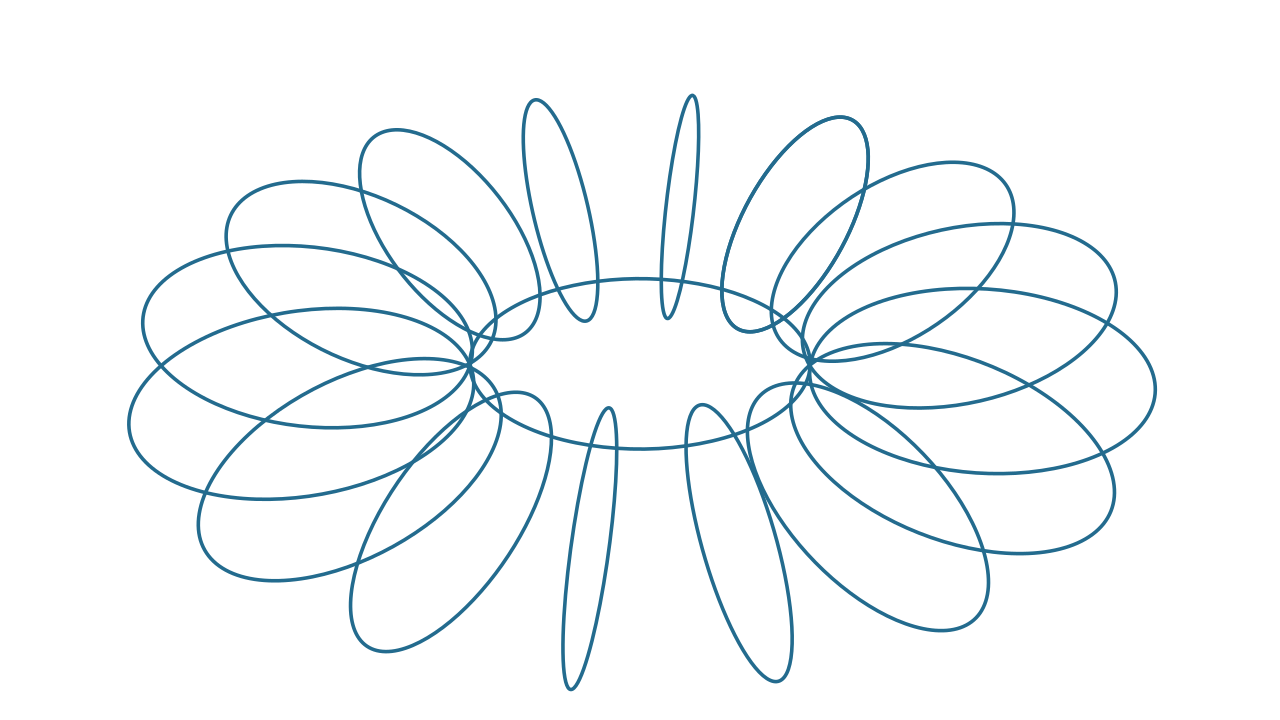
\includegraphics[width=0.5\linewidth]{pictures/TorusCircle_ManimCE_v0.18.1.png}
     \caption{Tore vu comme étant $\s{1}\times\s{1}$}
     \label{fig:torus-circle}
 \end{figure} 

La proposition nous permet de calculer le groupe fondamental du tore : \[\pi_1(T^2)=\pi_1(\s{1}\times\s{1})\cong\pi_1(\s{1})\times\pi_1(\s{1})\cong\bb{Z}^2\]Pour s'en persuader, il suffit de prendre deux générateurs : un lacet qui fait le tour de la "bouée", et un autre lacet qui fait le tour autour du trou. En notant $a$ le premier lacet et $b$ le second, on admet le fait qu'il existe une homotopie entre $ab$ et $ba$, qui intuitivement revient à décaler le moment où on effectue le tour de la bouée.

Nous pouvons généraliser ce calcul pour le tore à dimension $n>1$, définie comme étant $T^n=(\s{1})^n$. Son groupe fondamental est donc isomorphe à $\bb{Z}^n$.
\end{exemple}

Avec les outils que nous possédons dès à présent, il serait possible de calculer le groupe fondamental de la sphère de dimension quelconque. Nous allons plutôt voir un résultat plus fort, permettant de traiter ce cas de manière simple.

\subsection{Version faible du théorème de Van Kampen}

Si l'on peut décrire $X$ en tant que l'union de deux sous espaces $A$ et $B$, le théorème de Van Kampen stipule que l'on peut décrire son groupe fondamental en fonction de celui de $A$ et celui de $B$. Nous nous intéresserons à la version faible du théorème, c'est à dire lorsque $A\cap B$ forme un espace simplement connexe.

Mais avant de voir le théorème et ses applications, nous avons besoin d'introduire le produit libre de groupes.

\begin{definition}
Soient $G$ et $H$ deux groupes. Le \emph{produit libre} de $G$ et $H$, noté~$G\ast H$, est le l'ensemble des mots formé alternativement d'éléments de $G$ et d'éléments de $H$. On muni de la loi de concaténation, modulo les règles suivantes : \begin{itemize}
    \item Si une lettre est un élément neutre, alors elle est supprimée ;
    \item On a $(g)(g')=(gg')$ et $(h)(h')=(hh')$, pour tout $g,g'\in G$, et $h,h'\in H$.
\end{itemize}
Cela permet donc de former une loi de groupe sur cet ensemble $G\ast H$, avec l'élément neutre le mot vide, et l'inverse d'un mot comme étant le mot écrit à l'envers avec les inverses : $\Big((g_1)(h_1)\cdots(g_n)(h_n)\Big)\inv=(h_n\inv)(g_n\inv)\cdots(h_1\inv)(g_1\inv)$.
\end{definition}

\begin{exemple}
Soient $G=<g>$ et $H=<h>$. Les mots $ghg^2h^{-3}g^{12}, ghg^{-1}, hgh^2g^{-3}$ sont des exemples d'éléments appartenant au groupe $G\ast H$. L'inverse de $g^2h^3g^{-5}h$ est $h^{-1}g^5h^{-3}g^{-2}$.
\end{exemple}

\begin{theorem}[Van Kampen]\label{th:van-kampen}
Soit $X$ un espace, étant l'union de deux sous-espaces connexes par arc $A$ et $B$. Le morphisme $\pi_1(A)\ast\pi_1(B)\to\pi_1(X)$ est surjectif, et lorsque l'intersection $A\cap B$ est simplement connexe, il s'agit d'un isomorphisme.
\end{theorem}

L'idée est de décomposer les lacets de $X$ en des lacets de $A$ et des lacets de $B$. Le noyau du morphisme correspond au groupe fondamental de l'intersection, d'où le fait que l'on a un isomorphisme lorsque celui-ci est trivial. Pour une démonstration détaillé, le lecteur est invité à lire \href{https://www.normalesup.org/~fjacobe/Topo.pdf}{[TopoMa]}.

\subsubsection{Applications}
L'opérateur $\vee$, nommé \emph{bouquet} ou \emph{wedge sum} en anglais, sur les espaces permet de les joindre en un seul point. On obtient cet espace en effectuant le quotient de~$X\sqcup Y$ en identifiant deux points~$x_0\in X$ et~$y_0\in Y$.

\begin{exemple}
Le bouquet $\s{1}\vee\s{1}$, où l'on a identifié le point $(1,0)$ du premier cercle et le point $(-1,0)$ du second, nous donne une forme de $\infty$. Nous pouvons calculer son groupe fondamental grâce au théorème de Van Kampen.
\begin{figure}[H]
    \centering
    \begin{tikzpicture}
    \draw[thick, blue] (-1,0) circle (1cm) node{$A$};
    \draw[thick, red] (1,0) circle (1cm) node{$B$};
    \draw[thick, ->, blue] (0, 0) arc[start angle=0, end angle=110, radius=1]node[below left, near end]{$a$};
    \draw[thick, ->, red] (2, 0) arc[start angle=0, end angle=-110, radius=1]node[above left, near end]{$b$};
    \draw[thick, purple] (0,0) arc[start angle=0, end angle=-20, radius=1];
    \draw[thick, purple] (0,0) arc[start angle=0, end angle=20, radius=1];
    \draw[thick, purple] (0,0) arc[start angle=180, end angle=200, radius=1];
    \draw[thick, purple] (0,0) arc[start angle=180, end angle=160, radius=1];
    \draw[thick] (0,-1.3) arc[start angle=0, end angle=0, radius=1] node[below]{$X=A\cup B$};

    %A
    \draw[thick, blue] (5.5, 0) arc[start angle=0, end angle=360, radius=1]node[midway, right]{$A$};
    \draw[thick, blue] (5.5,0) arc[start angle=-20, end angle=0, radius=1];
    \draw[thick, blue] (5.5,0) arc[start angle=20, end angle=0, radius=1];
    %B
    \draw[thick, red] (6.5, 0) arc[start angle=180, end angle=-180, radius=1]node[midway, left]{$B$};
    \draw[thick, red] (6.5,0) arc[start angle=0, end angle=-20, radius=1];
    \draw[thick, red] (6.5,0) arc[start angle=0, end angle=20, radius=1];
    %AuB
    \draw[thick, purple] (6,0) arc[start angle=0, end angle=-20, radius=1];
    \draw[thick, purple] (6,0) arc[start angle=0, end angle=20, radius=1];
    \draw[thick, purple] (6,0) arc[start angle=180, end angle=200, radius=1] node[below] {$A\cap B$};
    \draw[thick, purple] (6,0) arc[start angle=180, end angle=160, radius=1];

    %arrow
    \draw[->, >=stealth, thick] (2.2,0) -- (3.3,0);
    \end{tikzpicture}
    \caption{Décomposition de $\s{1}\vee\s{1}$ pour le théorème de Van Kampen}
\end{figure}
Soit $X=\s{1}\vee\s{1}$, que nous décomposons comme sur la figure ci-dessus. Nous avons dans un premier temps les deux sous-espaces $A$ et $B$ homéomorphes au cercle. Leurs groupes fondamentaux sont donc également isomorphes à $\bb{Z}$. L'intersection $A\cap B$ est quant à elle simplement connexe, du fait qu'il s'agisse d'un point. Avec le théorème de Van Kampen, nous en déduisons le résultat suivant, en notant $x_0$ le point d'intersection des deux cercles : \[\pi_1(\s{1}\vee\s{1},x_0)\cong\pi_1(\s{1},(1,0))\ast\pi_1(\s{1},(-1,0))\cong\bb{Z}\ast\bb{Z}.\]En notant le lacet $a$ pour celui qui fait le tour du cercle bleu, et $b$ celui qui fait le tour du cercle rouge, nous avons bien deux générateurs libres du groupe. Il est important de remarquer ici que le groupe n'est pas abélien : il n'existe pas d'homotopie entre $ab$ et $ba$.
\end{exemple}

Nous pouvons alors calculer simplement le groupe fondamental de la sphère de dimension $n>1$.

\begin{proposition}
Pour $n>1$, la sphère $\s{n}$ est simplement connexe.
\end{proposition}
\begin{proof}
Montrons que le groupe fondamental de la sphère $\s{n}$ est trivial. Pour ce faire, nous considérons $A=\s{n}\setminus\{N\}$ et $B=\s{n}\setminus\{S\}$, avec $N$ et $S$ les points respectivement au nord et au sud de la sphère. Nous savons que $A$ et $B$ sont homéomorphes à $\bb{R}^n$, donc ces espaces sont simplement connexes.

Le théorème de Van Kampen, nous dit que le morphisme $0\ast0\to\pi_1(\s{n},x_0)$ est surjectif, ce qui nous permet de conclure que le groupe $\pi_1(\s{n},x_0)$ est trivial.
\end{proof}

La version forte du théorème est intéressante également, elle permet entre autres de calculer efficacement le groupe fondamental du plan projectif, avec un découpage astucieux (voir \href{https://www.math3ma.com/blog/the-fundamental-group-of-the-real-projective-plane}{[Math3ma]}). Pour ceux qui ne sont pas familier avec le plan projectif, je vous renvoie vers l'article \cite{Homeo-article} afin d'avoir une explication complète des différentes constructions. Voici tout de même une idée à avoir pour le calcul de son groupe fondamental.

\begin{exemple}
Initialement, le plan projectif réel $\bb{R}P^2$ désigne l'ensemble des droites vectorielles de~$\bb{R}^3$ passant par l'origine. Nous savons également qu'il peut être interprété comme le carré sur la figure~\ref{tkz:proj-plane}, et c'est cette représentation dont nous allons nous servir ici.


Notre objectif est d'avoir une représentation du groupe fondamental. Sur la figure \ref{tkz:proj-plane}, nous avons choisi comme point de base $x_0$ appartenant à la bordure. Comme il est identifié à son symétrique par rapport au centre du carré, il se trouve à la fois en haut à droite et à la fois en bas à gauche : c'est le même point ! Le chemin $\gamma$ traversant la diagonale désigne ainsi un exemple de lacet. Nous pouvons remarquer que nous ne pouvons pas rétracter ce lacet.

\begin{figure}[H]
\centering
\begin{subfigure}[t]{0.45\textwidth}
\centering
\begin{tikzpicture}[scale=.8]
    % fond gris
    \fill[gray!30] (0,0) rectangle (4,4);
    %flèche du haut
    \draw[thick, red, ->, >=stealth'] (0,4) -- (4,4) node[midway, below] {\textbf{A}};
    %flèche du bas
    \draw[thick, red, ->, >=stealth'] (4,0) -- (0,0) node[midway, above] {\textbf{A}};
    \draw[thick, blue, ->, >=stealth'] (0,0) -- (0,4) node[midway, right] {\textbf{B}};
    \draw[thick, blue, ->, >=stealth'] (4,4) -- (4,0) node[midway, left] {\textbf{B}};
    %carré
    \draw[black, line width=.0mm] (0,0) rectangle (4,4);
    
    %gamma
    \draw[thick, black, ->] (4,0) -- (2,2);
    \draw[thick, black] (2,2) -- (0,4) node[very near start, below]{$\gamma$};
    \filldraw[] (4,0) circle(1pt) node[right]{$x_0$};
    \filldraw[] (0,4) circle(1pt) node[left]{$x_0$};
\end{tikzpicture}
\caption{Le plan projectif et un lacet $\gamma$}
\label{tkz:proj-plane}
\end{subfigure}
\begin{subfigure}[t]{0.45\textwidth}
\centering
\begin{tikzpicture}[scale=.8]
    % fond gris
    \fill[gray!30] (0,0) rectangle (4,4);
    %flèche du haut
    \draw[thick, red, ->, >=stealth'] (0,4) -- (4,4) node[midway, below] {\textbf{A}};
    %flèche du bas
    \draw[thick, red, ->, >=stealth'] (4,0) -- (0,0) node[midway, above] {\textbf{A}};
    \draw[thick, blue, ->, >=stealth'] (0,0) -- (0,4) node[midway, right] {\textbf{B}};
    \draw[thick, blue, ->, >=stealth'] (4,4) -- (4,0) node[midway, left] {\textbf{B}};
    %carré
    \draw[black, line width=.0mm] (0,0) rectangle (4,4);
    \filldraw[] (4,0) circle(1pt) node[right]{$x_0$};
    \filldraw[] (0,4) circle(1pt) node[left]{$x_0$};
    %homotopie
    \draw[->] (4,0) -- (2,1.8);
    \draw[] (2,1.8) -- (0, 3.6);
    \draw[->] (4,0.4) -- (2,2.2);
    \draw[] (2,2.2) -- (0, 4);
    \draw[->, black!60] (4,0) -- (2,.2);
    \draw[black!60] (2,.2) -- (0, .4);
    \draw[->, black!60] (4,3.6) -- (2,3.8);
    \draw[black!60] (2,3.8) -- (0, 4);
    \draw[black!40] (4,0) arc[start angle=30, end angle=150, radius=1];
    \draw[->, black!40] (4,0) arc[start angle=30, end angle=90, radius=1];
    \draw[black!40] (0,4) arc[start angle=-150, end angle=-30, radius=1];
    %\draw[->, black!40] (0,4) arc[start angle=-150, end angle=-90, radius=1];
\end{tikzpicture}
\caption{Homotopie de $2\gamma$ vers le lacet constant}
\label{tkz:proj-plane-homotopy}
\end{subfigure}
\end{figure}
En revanche si l'on considère le lacet $2\gamma$, nous pouvons cette fois-ci le rétracter, en décalant au fur et à mesure le point de passage sur le côté B, pour atterrir sur le point de départ. Sur la figure~\ref{tkz:proj-plane-homotopy}, plus le lacet est clair, plus on avance sur l'homotopie.

\bigskip En terme plus formels, nous avons $[\gamma]\neq0$ et $2[\gamma]=0$, ce qui veut dire que le groupe généré par la classe d'homotopie de $\gamma$ est isomorphe à $\bb{Z}_2$. En réalité, $[\gamma]$ est la seule classe d'homotopie non triviale, ce qui fait que $\pi_1(\bb{R}P^2,x_0)\cong \bb{Z}_2$.
\end{exemple}

\subsection{Limitations du groupe fondamental}

Nous avons vu au préalable que le groupe fondamental était un bon outil de topologie algébrique, car il est invariant par équivalence d'homotopie, et par homéomorphisme. Néanmoins, dans une quête d'outils efficace, nous pouvons lui trouver plusieurs défauts. Le premier, et celui qui saute aux yeux, serait les groupes obtenus par cet outils. Ils ne sont pas abéliens ! Cela pose plusieurs soucis, comme notamment le fait que l'on puisse pas l'écrire sous forme d'un $\bb{Z}$-module, ou encore le fait que les sous-groupes ne sont pas tous normaux (et donc il est plus difficile de passer au quotient).

En plus de cela, il ne donne qu'un seul groupe, correspondant au comportement d'éléments de dimension 1, les lacets. Cela pourrait poser problème car il peut arriver bien souvent que des espaces ont le même groupe fondamental. Toutefois, il existe bien une généralisation du groupe fondamental pour les dimensions supérieures, mais comme nous allons le voir dans la partie suivante, ils ne donnent pas de résultats convenables ...

\subsubsection{Groupes d'homotopies de dimensions supérieures}

Sans rentrer dans les détails, il existe une généralisation du groupe fondamental pour les dimensions supérieures, que l'on appelle \emph{groupes d'homotopies}, et note $\pi_n$ pour la dimension $n$. Étrangement, à partir de la dimension 2, tous ces groupes sont abélien, contrairement au groupe fondamental.

Le problème majeur de ces groupes et qu'ils sont effroyablement compliqués à calculer, et nous donnent des résultats totalement inattendus. Une propriété que l'on aurait appréciée serait que pour un espace de dimension $n$, les groupes d'homotopies de dimensions supérieures soient triviaux... mais ce n'est pas le cas ici, comme le démontre le tableau suivant des premiers groupes d'homotopies des sphères.

\begin{figure}[H]
    \centering
    \small
    \begin{tabular}{|c|c|c|c|c|c|c|c|c|c|c|c|c|}
\hline
 & $\pi_1$ & $\pi_2$ & $\pi_3$ & $\pi_4$ & $\pi_5$ & $\pi_6$ & $\pi_7$ & $\pi_8$ & $\pi_9$ & $\pi_{10}$ & $\pi_{11}$ & $\pi_{12}$ \\
\hline
$\s{1}$ & $\mathbb{Z}$ & $0$ & $0$ & $0$ & $0$ & $0$ & $0$ & $0$ & $0$ & $0$ & $0$ & $0$\\
\hline
$\s{2}$ & $0$ & $\mathbb{Z}$ & $\mathbb{Z}$ & $\mathbb{Z}_2$ & $\mathbb{Z}_2$ & $\mathbb{Z}_{12}$ & $\mathbb{Z}_2$ & $\mathbb{Z}_2$ & $\mathbb{Z}_3$ & $\mathbb{Z}_{15}$ & $\mathbb{Z}_2$ & $\mathbb{Z}_{22}$ \\
\hline
$\s{3}$ & $0$ & $0$ & $\mathbb{Z}$ & $\mathbb{Z}_2$ & $\mathbb{Z}_2$ & $\mathbb{Z}_{12}$ & $\mathbb{Z}_2$ & $\mathbb{Z}_2$ & $\mathbb{Z}_3$ & $\mathbb{Z}_{15}$ & $\mathbb{Z}_2$ & $\mathbb{Z}_{22}$ \\
\hline
$\s{4}$ & $0$ & $0$ & $0$ & $\mathbb{Z}$ & $\mathbb{Z}_2$ & $\mathbb{Z}_2$ & $\mathbb{Z} \times \mathbb{Z}_{12}$ & $\mathbb{Z}_{22}$ & $\mathbb{Z}_{22}$ & $\mathbb{Z}_{24} \times \mathbb{Z}_3$ & $\mathbb{Z}_{15}$ & $\mathbb{Z}_2$ \\
\hline
$\s{5}$ & $0$ & $0$ & $0$ & $0$ & $\mathbb{Z}$ & $\mathbb{Z}_2$ & $\mathbb{Z}_2$ & $\mathbb{Z}_{24}$ & $\mathbb{Z}_2$ & $\mathbb{Z}_2$ & $\mathbb{Z}_2$ & $\mathbb{Z}_{30}$ \\
\hline
$\s{6}$ & $0$ & $0$ & $0$ & $0$ & $0$ & $\mathbb{Z}$ & $\mathbb{Z}_2$ & $\mathbb{Z}_2$ & $\mathbb{Z}_{24}$ & $0$ & $\mathbb{Z}$ & $\mathbb{Z}_2$ \\
\hline
$\s{7}$ & $0$ & $0$ & $0$ & $0$ & $0$ & $0$ & $\mathbb{Z}$ & $\mathbb{Z}_2$ & $\mathbb{Z}_2$ & $\mathbb{Z}_{24}$ & $0$ & $0$ \\
\hline
$\s{8}$ & $0$ & $0$ & $0$ & $0$ & $0$ & $0$ & $0$ & $\mathbb{Z}$ & $\mathbb{Z}_2$ & $\mathbb{Z}_2$ & $\mathbb{Z}_{24}$ & $0$ \\
\hline
$\s{9}$ & $0$ & $0$ & $0$ & $0$ & $0$ & $0$ & $0$ & $0$ & $\mathbb{Z}$ & $\mathbb{Z}_2$ & $\mathbb{Z}_2$ & $\mathbb{Z}_{24}$ \\
\hline
\end{tabular}
    \caption{Tableau des premiers groupes d'homotopies des sphères de dimensions 1 à 9}
    \label{fig:homotopy-groups-spheres}
\end{figure}

Il semble inutile de préciser que cela continue encore dans les dimensions supérieurs, et que les groupes obtenus sont encore plus inattendus.%gfd s^1, van kampen
%revetement, revetement universel, correspondance de Galois

\section{Revêtement, deuxième partie}

Nous avons introduit dans la partie \ref{covering-space-intro} la notion de revêtement, et ensuite vu comment elle pouvait nous aider à calculer le groupe fondamental du cercle. En réalité, la théorie sur les revêtements est bien plus profonde que cela, avec en autre un fort attachement à l'algèbre, avec une correspondance de Galois.

\subsection{Correspondance de Galois}

Tout d'abord, il faut comprendre qu'un espace ne possède pas qu'un seul revêtement. Avec l'exemple du cercle, nous avons choisi, lors du calcul du groupe fondamental \ref{th:grp-funda-circle}, la droite réelle, mais il en existe bien d'autres. Rien n'empêche le revêtement de faire deux tours au dessus du cercle, pour revenir au point de départ.
\begin{figure}[H]
\centering
\begin{subfigure}[b]{0.45\linewidth}
\centering
    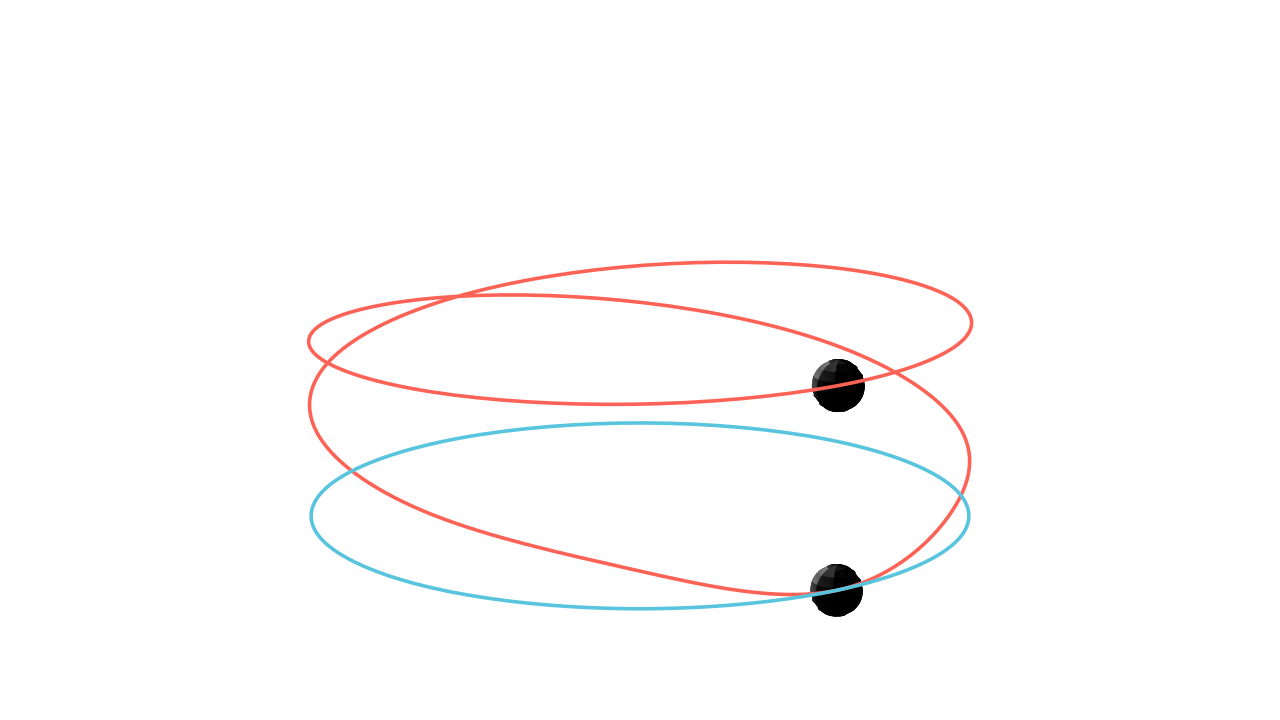
\includegraphics[width=.8\linewidth]{pictures/CoverCircle2_ManimCE_v0.18.1.png}
    \caption{\centering Exemple de revêtement (rouge) pour le cercle (bleu)}
    \label{fig:cover-circle-2}
\end{subfigure}
\hspace{5pt}
\begin{subfigure}[b]{0.45\linewidth}
\centering
    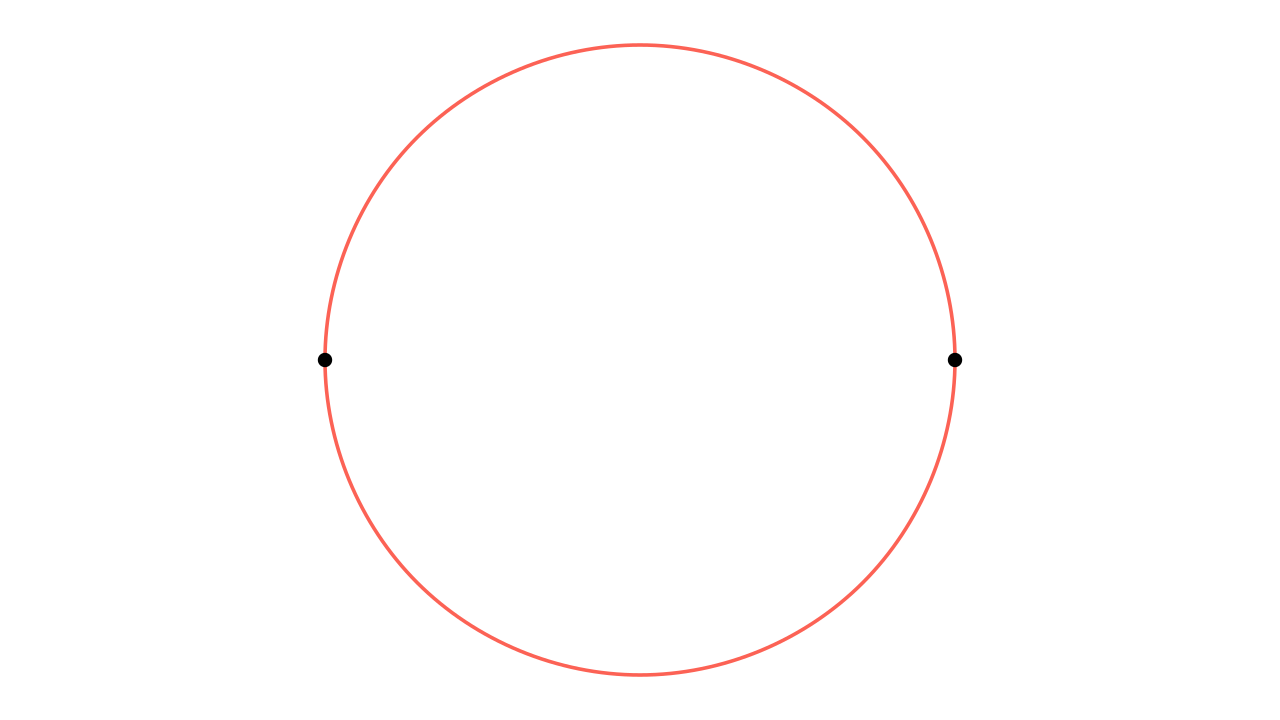
\includegraphics[width=.8\linewidth]{pictures/CoverCircle2_3_ManimCE_v0.18.1.png}
    \caption{\centering Revêtement vu comme un cercle, 2 fois plus long que l'original}
    \label{fig:cover-circle-2-2}
\end{subfigure}
\end{figure}

Pour cet exemple, nous pouvons supposer qu'il existe autant de revêtements qu'il existe d'entiers naturels... mais comment le démontrer ? C'est ce que nous allons voir par la suite.

\subsubsection{Énonce du théorème}

\begin{definition}
Un espace $X$ est \emph{localement connexe par arc} si pour tout voisinage de~$x\in X$, il existe un voisinage inclut dans le premier tel que celui-ci est connexe par arc.

Un espace est dit \emph{semi-localement simplement connexe} si pour tout voisinage de tout point $x\in X$, les lacets dans ce voisinage sont homotopes au lacet constant une fois plongés dans $X$. Autrement dit, le groupe fondamental du voisinage devient trivial dans $X$.
\end{definition}

\begin{exemple}
Un espace avec deux composantes connexes par arc disjointes est localement connexe par arc : il suffit de prendre un voisinage se trouvant dans une seule des deux composantes.

Tout espace simplement connexe est semi-localement simplement connexe. Par exemple, avec~${X=D^2}$, si l'on prend un voisinage étant homéomorphe à une couronne (ie. il possède un trou), son groupe fondamental est certes non trivial, mais une fois plongé dans l'espace $X$, les classes d'homotopies sont toutes égales à celle du lacet constant.
\end{exemple}

Un morphisme entre deux revêtements $p_1:\Tilde{X}_1\to X$ et $p_2:\Tilde{X}_2\to X$ est une application~${f:\Tilde{X}_1\to\Tilde{X}_2}$, amenant un point de base $\Tilde{x}_1\in p_1\inv(x_0)$ vers un point de base $\Tilde{x}_2\in p_2\inv(x_0)$.

\begin{theorem}
Pour un espace pointé $(X,x_0)$ connexe par arc, localement connexe par arc, et semi-localement simplement connexe, il existe une bijection entre :\begin{itemize}
    \item les sous groupes de $\pi_1(X,x_0)$ ;
    \item les revêtements $p:(\Tilde{X},\Tilde{x}_0)\to(X,x_0)$, à isomorphisme près de revêtements, conservant le point de base ;
\end{itemize} obtenue en associant le groupe $p_\ast(\pi_1(\Tilde{X},\Tilde{x}_0))$ au revêtement $(\Tilde{X},\Tilde{x}_0)$.
\end{theorem}

Pour la démonstration nous allons tout d'abord montrer que le morphisme induit $p_\ast$ est injectif, puis nous allons construire le revêtement lié au sous groupe trivial. Par la suite, nous montrerons que nous pourrons associer un revêtement à un sous groupe du groupe fondamental, pour enfin voir que les classes d'isomorphismes de revêtements induisent le même morphisme.

\subsubsection{Démonstration}

Nous considérons au cours de cette partie un espace pointé $(X,x_0)$ connexe par arc, localement connexe par arc, et semi-localement simplement connexe.

\begin{proposition}
Pour un revêtement $p:(\Tilde{X},\Tilde{x}_0)\to(X,x_0)$, le morphisme induit $p_\ast$ est injectif.
\end{proposition}
\begin{proof}
Le morphisme $p_\ast$ envoie $[\Tilde{\gamma}]\in\pi_1(\Tilde{X},\Tilde{x}_0)$ vers $[p\Tilde{\gamma}]\in\pi_1(X,x_0)$. Soit $[\Tilde{\gamma}]\in\ker(p_\ast)$, c'est à dire que $p\Tilde{\gamma}$ est homotope au lacet constant. Par relèvement d'homotopie, le lacet $\Tilde{\gamma}$ est homotope au lacet constant dans $(\Tilde{X},\Tilde{x}_0)$.
\end{proof}

\begin{definition}
Un revêtement simplement connexe est appelé \emph{revêtement universel}, et comme il est unique à isomorphisme près avec la correspondance de Galois, nous l'appelons le revêtement universel.
\end{definition}

\begin{proposition}
Pour $X$ un espace connexe par arc, localement connexe par arc, et semi-localement simplement connexe, il existe un revêtement universel.
\end{proposition}
La démonstration se fait par construction du revêtement et d'une topologie adéquate. Pour définir une topologie sur le revêtement, nous allons construire une base de topologie.

\begin{definition}
Une \emph{base de topologie} sur un ensemble $Y$ est une collection $\mathcal{B}$ telle que :\begin{enumerate}
    \item $Y=\bigcup_{V\in B}V$ ;
    \item Pour $U,U'\in \mathcal{B}$ et $y\in U\cap U'$, il existe un $V\in\mathcal{B}$ tel que $y\in V\subseteq U\cap U'$.
\end{enumerate}
En notant $\mathcal{T}$ l'ensemble des des sous-ensembles de $Y$ pouvant être écrit comme union d'éléments de~$\mathcal{B}$, alors $\mathcal{T}$ est une topologie de $Y$.
\end{definition}
Nous pouvons désormais commencer la démonstration.
\begin{proof}
Nous considérons l'ensemble $\Tilde{X}=\{[\gamma],\gamma\text{ chemin de $X$, $\gamma(0)=x_0$}\}$ et l'application~${p:\Tilde{X}\to X, [\gamma]\mapsto\gamma(1)}$. Nous allons montrer que le couple $(\Tilde{X},p)$ est un revêtement de $X$ simplement connexe.

L'application $p$ est bien définie, puisque pour $\gamma\simeq\gamma'$, nous avons les extrémités qui sont conservées. De plus, l'application est surjective puisque $X$ est connexe par arc.

\bigskip Pour définir une base de topologie sur $\Tilde{X}$, nous allons commencer par en trouver une adéquate pour $X$. Ensuite nous allons montrer qu'avec cette base, la projection définie un revêtement, notamment avec l'image réciproque qui est une union disjointe d'ouvert de $\Tilde{X}$. Enfin, nous montrerons que ces ouverts forment une base de topologie sur $\Tilde{X}$.

Tout d'abord, comme $X$ est un espace localement connexe par arc et semi-localement simplement connexe, l'ensemble des ouverts connexes par arc tel que leurs groupes fondamentaux sont triviaux dans $X$ forme un recouvrement, que l'on note : \[B_X=\{U\subset X \text{ouvert connexe par arc et } i_\ast(\pi_1(U))=1\in\pi_1(X)\}.\]Montrons que ceci forme une base de topologie de $X$. Soient deux ouverts $U,U'\in\mathcal{B}_X$, et soit un point $x\in U\cap U'$. Par la connexité parc arc locale, nous savons qu'il existe $V\subseteq U\cap U'$ tel que $V$ soit connexe par arc. De plus, puisque $V\subset U$, nous avons la chaîne d'inclusion $V\hookrightarrow U\hookrightarrow X$ qui induit un morphisme sur les groupes fondamentaux. Comme $\pi_1(U)\mapsto 1\in \pi_1(X)$, il en est de même pour~$V$. Nous en déduisons alors que $V\in \mathcal{B}_X$. Nous pouvons ainsi conclure que l'ensemble $\mathcal{B}_X$ forme une base de topologie de $X$.

Soit $U_i\in\mathcal{B}_X$. Étant donné que son groupe fondamental est trivial dans $X$, chaque classe d'homotopie de chemins est uniquement déterminée par ses extrémités. Si l'on fixe le point de départ, à~$x_0$ par exemple, nous obtenons ainsi une union disjointe :$$p\inv(U_i)=\bigsqcup_{x\in U_i}\{[\gamma],\gamma\text{ chemin de $U_i$ tel que }\gamma(0)=x_0,\gamma(1)=x\}.$$Cet union est bien trop gros et ne peut formé une base de topologie sur $\Tilde{X}$. Nous définissons alors une relation sur les classes d'homotopies de chemins : $[\gamma]\approx[\gamma']$ si et seulement s'il existe $\eta$ un chemin de~$U_i$ tel que $\gamma\cdot\eta=\gamma'$. Il n'est pas difficile de vérifier que cette relation est une relation d'équivalence. Nous noterons $V_{ij}$ l'ensemble des classes d'équivalences de $\approx$ sur $U_i$, indexé par $j$. Nous obtenons alors une union disjointe avec ces ensembles : \[p\inv(U_i)=\bigsqcup_{j}V_{ij}=\bigsqcup_j\{[\gamma\cdot\eta],\eta\text{ chemin de $U_i$ avec $\eta(0)=\gamma(1)$}\}.\]Soit $V_{ij}\in p\inv(U_i)$. Montrons que $p:V_{ij}\to U_i$ est une bijection. Il est clair que l'application est surjective, puisque $U_i$ est connexe par arc. Pour montrer qu'elle est injective, supposons que l'on ait~$p([\gamma\cdot\eta])=p([\gamma'\cdot\eta'])$. Par définition de $p$, nous avons $\eta(1)=\eta'(1)$. Par simple connexité semi locale, les deux chemins $\gamma\cdot\eta$ et $\gamma'\cdot\eta'$ sont homotopes, car possède les mêmes extrémités. Autrement dit, nous avons $[\gamma\cdot\eta]=[\gamma'\cdot\eta']$, ce qui fait de $p$ une application injective.

Il reste à démontrer que les $V_{ij}$ forment une base de topologie de $\Tilde{X}$. Nous noterons cet ensemble ainsi : $$\mathcal{B}_{\Tilde{X}}=\bigcup_ip\inv(U_i)=\bigcup_{i,j}V_{ij}.$$ Il est clair que cela forme un recouvrement de $\Tilde{X}$. Soit $V_{ij},V_{i'j'}\in\mathcal{B}_{\Tilde{X}}$ deux ouverts de cet ensemble, avec $\Tilde{x}\in V_{ij}\cap V_{i'j'}$. Il existe, par définition de la base de topologie de $X$, un ouvert $U\in \mathcal{B}_X$ tel que~${p(y)\in U\subset U_i\cap U_{i'}=p(V_{ij})\cap p(V_{i'j'})}$. Par définition, la relation d'équivalence sur $U$ implique la relation sur $U_i$ et $U_j$. Ainsi, la classe d'équivalence $V\in p\inv(U)$ contenant $y$ vérifie $V\subset V_{ij}\cap V_{i'j'}$. Ainsi, nous avons montré que $B_{\Tilde{X}}$ est une base de topologie sur $\Tilde{X}$. Il est assez facile de voir qu'avec ces bases de topologie, $p:\Tilde{X}\to X$ est un revêtement : l'image réciproque de tout ouvert de $\mathcal{B}_X$ est dans $\mathcal{B}_{\Tilde{X}}$ (continuité de $p$), et toute image d'ouvert de $\mathcal{B}_{\Tilde{X}}$ est un ouvert de $\mathcal{B}_X$ (montrant la continuité de la réciproque, et donc l'homéomorphisme $p:V_{ij}\to U_i$).

\bigskip Il nous reste alors plus qu'à montrer la simple connexité de $\Tilde{X}$. Tout d'abord, nous pouvons remarquer que $\Tilde{X}$ est connexe par arc, puisqu'il existe un chemin entre $[x_0]$, le chemin constant basé en $x_0$, et $[\gamma]\in \Tilde{X}$ : il suffit de prendre le chemin~$[\gamma|_{[0,t]}], t\in[0,1]$. Pour la simple connexité, on considère un lacet~$f$ de $\Tilde{X}$ basé en $[x_0]$, et on note $pf=\gamma$, un lacet basé en $x_0$. Si on note le chemin $\gamma_t=~\gamma|_{[0,t]}$, de telle sorte que $[\gamma_t]$ est un relèvement de $\gamma$, nous avons~$[\gamma_0]=[x_0]=f(0)$. Par unicité du relèvement, nous obtenons $[\gamma_t]=f(t)$, et en particulier l'égalité~$[\gamma_1]=f(1)=[x_0]$. Comme $\gamma_1=\gamma$, on en déduit $[\gamma]=[x_0]$ : la projection $pf=\gamma$ est homotope au lacet constant. Par injectivité de $p_\ast$, nous avons~$p_\ast([f])=0$ qui implique $[f]=0$, d'où le fait que $\Tilde{X}$ soit simplement connexe.
\end{proof}

Cette construction théorique est efficace car elle permet d'affirmer l'existence du revêtement universel pour un espace vérifiant les propriétés demandées. De plus, elle permet de démontrer d'autres résultats théoriques, comme la proposition qui suit. En revanche, lors de calculs concrets, ce n'est pas cette méthode qui est utilisée (il suffit de voir le revêtement universel du cercle).

\begin{proposition}
Soit $X$ un espace connexe par arc, localement connexe par arc, et semi-localement simplement connexe. Pour chaque $H$ sous groupe de~$\pi_1(X,x_0)$, il existe un revêtement~${p:X_H\to X}$, tel que $p_\ast(\pi_1(X_H,\Tilde{x}_0))=H$, pour un certain $\Tilde{x}_0\in X_H$.
\end{proposition}
\begin{proof}
On définit tout d'abord une relation sur le revêtement universel $\Tilde{X}$ de~$X$ : \[[\gamma]\approx[\gamma']\Longleftrightarrow\gamma(1)=\gamma'(1)\text{ et }[\gamma\cdot\overline{\gamma'}]\in H.\]Il est facile de voir qu'il s'agit d'une relation d'équivalence, nous allons pouvoir passer au quotient et définir $p:X_H\to X$ avec $X_H=X/\approx$.

Nous choisissons comme point de base $\Tilde{x}_0\in X_H$, la classe d'équivalence du chemin constant~$c$ en~$x_0$. Montrons que $p_\ast(\pi_1(X_H,\Tilde{x}_0))=H$. Étant donné un lacet $\gamma$ de $(X,x_0)$, il se relève en un chemin de $[c]$ vers $[\gamma]$. Pour que l'image du relèvement de $\gamma$ sur $X_H$ soit un lacet, il faut que~$[\gamma]\approx[c]$. Autrement dit, il faut que $[\gamma]\in H$.
\end{proof}

Il nous reste à démontrer que les revêtements correspondant à un même sous-groupe sont identiques, à isomorphisme près.

\begin{proposition}
Soit $X$ un espace connexe par arc, localement connexe par arc, et semi-localement simplement connexe. Deux revêtements sont isomorphes si et seulement si les sous-groupes induits par l'image du morphisme induit par leurs projections sont identiques.
\end{proposition}

\begin{proof}
Soient $p_1:(\Tilde{X}_1,\Tilde{x}_1)\to (X,x_0)$ et $p_2:(\Tilde{X}_2,\Tilde{x}_2)\to (X,x_0)$, avec~$\Tilde{x}_1\in p_1\inv(x_0)$ et~${\Tilde{x}_2\in p_2\inv(x_0)}$. Montrons que ces revêtements sont isomorphes ssi ${p_{1\ast}(\pi_1(\Tilde{X}_1,\Tilde{x}_1))=p_{2\ast}(\pi_1(\Tilde{X}_2,\Tilde{x}_2)}$.

Supposons que les revêtements soient isomorphes via $f:\Tilde{X}_1\to \Tilde{X}_2$. Nous avons alors les égalités~${p_1=p_2f}$ et $p_2=p_1f\inv$. L'application $f$ induit un isomorphisme $f_\ast:\pi_1(\Tilde{X}_1,\Tilde{x}_1)\to \pi_1(\Tilde{X}_2,\Tilde{x}_2)$, de telle sorte que $p_{1\ast}f_\ast=p_{2\ast}$ et $p_{2\ast}f\inv_\ast=p_{1\ast}$, ce qui nous donne : \[p_{2\ast}(\pi_1(\Tilde{X}_2,\Tilde{x}_2))=p_{1\ast}f_\ast(\pi_1(\Tilde{X}_2,\Tilde{x}_2))=p_{1\ast}(\pi_1(\Tilde{X}_1,\Tilde{x}_1)),\] ainsi que \[p_{1\ast}(\pi_1(\Tilde{X}_1,\Tilde{x}_1))=p_{2\ast}f\inv_\ast(\pi_1(\Tilde{X}_1,\Tilde{x}_1))=p_{2\ast}(\pi_1(\Tilde{X}_2,\Tilde{x}_2)).\]

Supposons désormais que les sous-groupes induits sont identiques. Par le critère de relèvement, il existe $\Tilde{p}_1:(\Tilde{X}_1,\Tilde{x}_1)\to(\Tilde{X}_2,\Tilde{x}_2)$, tel que $p_2\Tilde{p}_1=p_1$. De même, il existe $\Tilde{p}_2:(\Tilde{X}_2,\Tilde{x}_2)\to(\Tilde{X}_1,\Tilde{x}_1)$, avec $p_1\Tilde{p}_2=p_2$. Par unicité du relèvement, nous avons $\Tilde{p}_1\Tilde{p}_2=id$ et $\Tilde{p}_2\Tilde{p}_1=id$, ce qui fait de $\Tilde{p}_1$ et $\Tilde{p}_2$ des isomorphismes.
\end{proof}

Finalement, avec ces trois propositions, nous avons toutes les cartes pour démontrer le théorème.

\bigskip Néanmoins, il reste un fait algébrique intéressant, renforcant le lien de la correspondance de Galois.

\begin{proposition}
Soit $X$ un espace, et $(\Tilde{X},p)$ un revêtement de $X$. On appelle \emph{fibre}, ou feuillet, de $x_0\in X$, un élément de $p\inv(x_0)$. Le nombre de fibres est constant pour tout $x_0\in X$, et est égal à l'indice du sous groupe $p_\ast(\pi_1(\Tilde{X},\Tilde{x}_0))$, avec $\Tilde{x}_0\in p\inv(x_0)$.
\end{proposition}

L'idée de la démonstration est de montrer que pour tout élément du recouvrement $U_i\in X$, le cardinal de $p\inv (U_i)$ ne dépend pas du choix de $U_i$. Cela vient du fait que les $U_i$ peuvent se chevaucher, ayant alors le même cardinal pour l'image réciproque.

\begin{exemple}
Reprenons l'exemple du cercle. Son revêtement universel est celui dont nous nous sommes servi pour la démonstration, à savoir $\bb{R}$, puisqu'il est simplement connexe. Avec la dernière proposition et le théorème, nous pouvons déduire que le revêtement avec $n$ feuillets est en bijection avec le sous-groupe $n\bb{Z}$ dans $\pi_1(\s{1},(1,0))$, car $[\bb{Z}:n\bb{Z}]=|\bb{Z}_n|=n$.
\end{exemple}

\subsection{Transformation de deck}

Pour un revêtement $p:\Tilde{X}\to X$, on appelle \emph{transformation de deck}, ou transformation de revêtement, tout isomorphisme $\Tilde{X}\to\Tilde{X}$. Il est important de voir que pour conserver la structure du revêtement, toute les opérations sur un espace (comme les symétries) ne sont pas autorisées. La transformation doit en autres conserver l'ordre des feuillets (voir figure \ref{fig:deck-transformation}). De ce fait, et de la propriété d'unicité du relèvement, la transformation est entièrement déterminée par la transformation d'un point (les autres suivront la même transformation).

\begin{figure}[H]
    \centering
    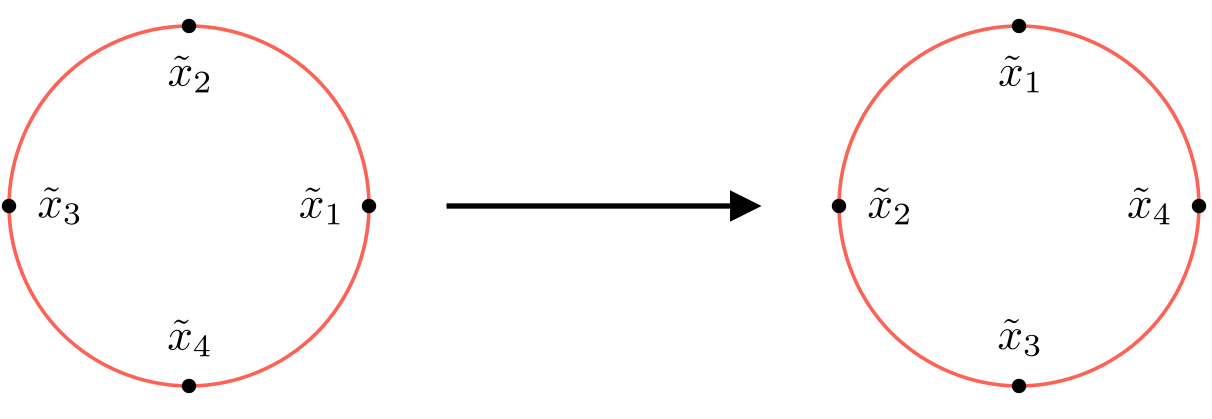
\includegraphics[width=0.5\linewidth]{pictures/CoverCircle2_2_ManimCE_v0.18.1.png}
    \caption{Exemple de transformation de deck}
    \label{fig:deck-transformation}
\end{figure}

L'ensemble des transformations de deck d'un revêtement $\Tilde{X}$, noté généralement $G(\Tilde{X})$, possède en réalité une structure de groupe. Muni de la composition d'isomorphismes, il est clair que l'élément neutre est l'application l'identité, que les transformations admettent un symétrique, et que la loi est associative. 

De plus, on dit qu'un revêtement est \emph{normal} si pour tout $x\in X$, tout couple~$(\Tilde{x},\Tilde{x}')\in p\inv(x)$, il existe une transformation passant de~$(\Tilde{X},\Tilde{x})$ à $(\Tilde{X},\Tilde{x}')$.

\begin{exemple}
Pour un revêtement du cercle à $n$ feuillets, les transformations de deck sont les isomorphisme $\varphi_k:z\mapsto z^k$ pour $k\in\bb{Z}^*$. Nous pouvons remarquer que l'on a $\varphi_k=\varphi_{an+k}$, pour $a$ entier. D'où la conjecture du fait que~$G(\Tilde{X})\cong\bb{Z}_n$.
\end{exemple}

Les transformations de deck ont un lien très étroit avec la correspondance de Galois, comme peut nous le montrer la proposition qui suit : 

\begin{proposition}
Soit $p:(\Tilde{X},\Tilde{x}_0)\to(X,x_0)$ un revêtement connexe par arc d'un espace $X$ connexe par arc et localement connexe par arc. En notant le sous-groupe $H=p_\ast(\pi_1(\Tilde{X},\Tilde{x}_0))$ de~$\pi_1(X,x_0)$, nous avons : \begin{itemize}
    \item Le revêtement est normal si et seulement si $H$ est un sous-groupe normal ;
    \item Le groupe $G(\Tilde{X})$ est isomorphe à $N(H)/H$, où $N(H)$ est le normalisateur.
\end{itemize}
En particulier, si $\Tilde{X}$ est un revêtement normal, alors $G(\Tilde{X})\cong \pi_1(X,x_0)/H$.
\end{proposition}

\textbf{[insérer preuve]}

Les transformations de deck sont un cas particulier de ce que l'on appelle une action de groupe sur un espace.

\begin{definition}\label{def:group-action}
Une action de groupe $G$ sur un espace $X$ est un morphisme $\rho$ de $G$ vers le groupe des homéomorphismes de $X$ dans lui-même, noté~$Homeo(X)$. Ce morphisme est définie pour $g\in G$ par $\rho(g):X\to X$, que l'on simplifiera par $g:X\to X$.
\end{definition}

\begin{remark}
En reprenant les notations de l'énoncé, étant donné que $\rho$ est un morphisme, alors il vérifie $e_G(x)=x$ pour $e_G$ l'élément neutre, pour et $x\in X, g,g'\in G, {g(g'(x))=(gg')(x)}$.
\end{remark}

Il existe également des actions de groupe sur un ensemble quelconque, qui se définissent de manière presque similaire, mais ce ne sont pas ceux qui nous intéresse ici.

\subsubsection{Propriétés sur les actions de groupes}

Une question que l'on pourrait se poser sur les actions de groupes, serait de savoir si elles peuvent représenter des transformations de deck. Il suffirait en effet qu'elles vérifient quelques propriétés pour que ce soit le cas.

\begin{definition}
Étant donné un groupe $G$ et $Y$ un espace, on appelle \emph{orbite} de $y\in Y$ l'ensemble~$Gy=\{g(y),g\in G\}$. L'ensemble des orbites ${Y/G=\{Gy,y\in Y\}}$ est appelé \emph{espace des orbites}
\end{definition}

\begin{exemple}
Pour un revêtement normal, l'espace des orbites $\Tilde{X}/G(\Tilde{X})$ est $X$.
\end{exemple}

Pour une action de groupe $G$ sur l'espace $Y$, notons cette propriété :

\begin{equation}\label{eq:prop-action}
\forall y\in Y,\exists U\in\mathcal{V}(y),\forall g,g'\in G, g(U)\cap g'(U)\neq\emptyset\Longrightarrow g=g'
\end{equation}

Cette propriété est vérifiée par les transformations de deck. De plus, si la propriété est vérifiée, elle permet alors de retomber sur des revêtements. 

\begin{proposition}
Si une action de groupe $G$ sur $Y$ vérifie \eqref{eq:prop-action}, alors :\begin{itemize}
    \item L'application quotient $p:Y\to Y/G$ est un revêtement normal :
    \item Si $Y$ est connexe par arc, alors $G$ est le groupe de transformations de deck du revêtement~${Y\to Y/G}$ ;
    \item Si $Y$ est connexe par arc et localement connexe par arc, alors $G\cong\pi_1(Y/G)/p_\ast(\pi_1(Y))$.
\end{itemize}
\end{proposition}

Une autre question pourrait se poser désormais : quand est-ce qu'une action de groupe vérifie la propriété \eqref{eq:prop-action} ?

\begin{definition}
Une action vérifiant uniquement l'élément neutre comme point fixe est appelée \emph{action libre}.

Une action de groupe $G$ sur $Y$ possède la propriété de \emph{discontinuité propre} si elle vérifie : \[\forall y\in Y,\exists U\in\mathcal{V}(y), |\{g\in G,U\cap g(U)\neq\emptyset\}|<+\infty\]
\end{definition}

\begin{proposition}
Soit $G$ une action de groupe sur $Y$.\begin{itemize}
    \item Si l'action de groupe vérifie \eqref{eq:prop-action}, alors c'est une action libre.
    \item Si $Y$ est Hausdorff, et que l'action est libre et vérifie la discontinuité propre, alors elle vérifie~\eqref{eq:prop-action}.
\end{itemize}
\end{proposition}
\begin{proof}
La première affirmation est évidente.
\end{proof}

\begin{comment}
\begin{proof}
Soit $G$ une action de groupe libre et vérifiant la discontinuité propre sur un espace Hausdorff $Y$. Soit $y\in Y$, et soient deux éléments différents $g,g'\in G$. Notons $y'=g\inv g'(y)$, dont nous savons que $y\neq y'$ du fait que l'action soit libre. Ainsi, le voisinage de $y'$ s'exprime en fonction de celui de $y$. Du fait que l'espace soit Hausdorff, nous savons qu'il existe un ouvert $V\in\mathcal{V}(y)$, avec~$V'=g\inv g'(V)\in\mathcal{V}(y')$, tel que $V\cap V'=V\cap g\inv g'(V)=0$.

Si l'on répète le processus pour tout couples $(g,g')\in G^2$, nous obtenons une famille d'ouvert. Il suffit de prendre l'intersection de ceux-ci pour trouver notre ouvert $U$ vérifiant \eqref{eq:prop-action}.
\end{proof}
\end{comment}

\begin{exemple}
Les actions de groupes finis vérifie la discontinuité propre automatiquement, alors il suffit que ce soit une action libre pour pouvoir vérifier \eqref{eq:prop-action}.
\end{exemple}%reveêtement et galois
\chapter{Homologie : enfin abélien !}\label{chp:homology}
%delta complexe, homologie simpliciale 

Comme il est annoncé dans le titre, nous allons enfin pouvoir manipuler seulement des groupes abéliens. C'est le plus gros avantage à travailler sur l'homologie plutôt que sur le groupe fondamental. Un autre point fort de cet outil et que les groupes de dimensions supérieurs à l'espace sont triviaux, ce qui n'est pas le cas des groupes d'homotopies (voir le tableau \ref{fig:homotopy-groups-spheres}). En revanche, ce confort de manipulation à un coût : une plus forte abstraction des outils utilisés.

L'homologie peut être perçue comme étant l'abélianisation du groupe fondamental (voir section~\ref{sect:abelianisation} pour la démonstration), mais qu'est ce que cela représente concrètement ? Heureusement, la simplicité des calculs viendra contrebalancer les difficultés que nous pourrions avoir à appréhender le concept profond de l'homologie.

\bigskip Nous allons le voir rapidement, il existe différentes homologies, définies de façons différentes. Après les avoir introduits, ainsi que de voir leurs avantages et défauts, nous verrons qu'elles sont finalement isomorphes. Afin de mieux appréhender ces notions, nous allons commencer par l'homologie qui est la plus géométrique : l'homologie simpliciale.

\section{Homologie simpliciale : triangularisation}

L'homologie simpliciale ce calcule après avoir effectué une triangularisation de l'espace. Nous allons définir formellement comment obtenir une telle structure, en commençant par une généralisation des triangles.

\subsection{Des simplexes et des $\Delta$-complexes}\label{sect:simplices}
Intuitivement, un \emph{simplexe} est une généralisation du triangle, mais à n'importe quelle dimension. En dimension 1 il s'agit d'un segment, en dimension 2 un triangle, et en dimension 3 un tétrahèdre. Formellement, voici comme il est défini.

\begin{wrapfigure}{l}{0.3\textwidth}
\centering
\begin{tikzpicture}
\begin{scope}[thick,decoration={markings, mark=at position 0.5 with {\arrow{stealth}}}] 
    \draw[postaction={decorate}] (1,4.5)--(3,5.5);
    %2-simplex
    \draw[postaction={decorate}] (-.5,3)--(1,3);
    \draw[postaction={decorate}] (1,3)--(.5,4);
    \draw[postaction={decorate}] (-.5,3)--(.5,4);
    %3-simplex
    \draw[postaction={decorate}] (1.5,3)--(2.5,2.5);
    \draw[postaction={decorate}] (1.5,3)--(3.3,3.2);
    \draw[postaction={decorate}] (1.5,3)--(2.5,4);
    \draw[postaction={decorate}] (2.5,2.5)--(3.3,3.2);
    \draw[postaction={decorate}] (2.5,2.5)--(2.5,4);
    \draw[postaction={decorate}] (3.3,3.2)--(2.5,4);
\end{scope}
%0-simplex
\filldraw[] (0,5) circle(1pt) node[below]{$v_0$};
%1-simplex
\filldraw[] (1,4.5) circle(1pt) node[below]{$v_0$};
\filldraw[] (3,5.5) circle(1pt) node[below]{$v_1$};
%2-simplex
\filldraw[] (-.5,3) circle(1pt) node[below left]{$v_0$};
\filldraw[] (1,3) circle(1pt) node[below]{$v_1$};
\filldraw[] (.5,4) circle(1pt) node[above left]{$v_2$};
%3-simplex
\filldraw[] (1.5,3) circle(1pt) node[below]{$v_0$};
\filldraw[] (2.5,2.5) circle(1pt) node[below]{$v_1$};
\filldraw[] (3.3,3.2) circle(1pt) node[below]{$v_2$};
\filldraw[] (2.5,4) circle(1pt) node[above right]{$v_3$};

\end{tikzpicture}
\caption{\centering Simplexes de dimensions 0 à 3}
\label{tkz:simplex}
\end{wrapfigure}
\phantom{cyrille le goat}

\begin{definition}
Étant donné $n+1$ points~$v_0,...,v_n\in\bb{R}^m$ tels que les vecteurs~$v_i-v_0$ soient linéairement indépendant, un \emph{$n$-simplexe} est le plus petit ensemble convexe contenant tout ces points, que l'on note $[v_0,...,v_n]$. Les points $v_i$ sont appelés les \emph{sommets} du simplexe, et les sous-simplexes obtenu par le retrait d'un ou plusieurs sommets sont appelés les \emph{faces} du simplexe.
\end{definition}

\begin{remark}
Les simplexes possèdent des faces orientés. Par convention, l'ordre indiqué dans le nom de simplexe indique le sens des flèches. Par exemple, $[v_0,v_1]$ est un segment orienté de $v_0$ et $v_1$.
\end{remark}

\begin{exemple}
On définit le \emph{simplexe standard} par : \[\Delta^n=\left\{(t_0,...,t_n)\in\bb{R}^{n+1},\sum_{i=0}^nt_i=1,t_i\geq0,\forall i=0,...,n\right\}\]
\end{exemple}

\begin{definition}
Un $\Delta$-simplexe est un espace obtenu par une union de simplexes de différentes dimensions, auquel on identifie des faces via un homéomorphisme laissant invariant l'ordre les côtés.
\end{definition}

\begin{exemple}
Voici une représentation du tore en deux dimensions, du plan projectif réel, et de la bouteille de Klein, en tant que $\Delta$-complexes. Attention, ce ne sont pas les seules décompositions qui existent !

\begin{figure}[H]
\centering
\begin{subfigure}[t]{0.3\textwidth}
\centering
\begin{tikzpicture}[scale=.6]
% fond gris
\fill[gray!30] (0,0) rectangle (4,4);
\begin{scope}[thick,decoration={markings, mark=at position 0.5 with {\arrow{stealth}}}] 
    \draw[postaction={decorate}, red] (0,4)--(4,4)node[midway, below] {$a$};
    \draw[postaction={decorate}, red] (0,0)--(4,0) node[midway, above] {$a$};
    \draw[postaction={decorate}, blue] (0,0)--(0,4) node[midway, right] {$b$};
    \draw[postaction={decorate}, blue] (4,0)--(4,4) node[midway, left] {$b$};
    \draw[postaction={decorate}, brown] (4,0) -- (0,4)node[midway, below]{$c$};
\end{scope}
    \filldraw[] (4,0) circle(1pt) node[right]{$x_0$};
    \filldraw[] (0,4) circle(1pt) node[left]{$x_0$};
    \filldraw[] (4,4) circle(1pt) node[right]{$x_0$};
    \filldraw[] (0,0) circle(1pt) node[left]{$x_0$};
    \filldraw[gray] (1,1) circle(0pt) node[]{$\sigma_1$};
    \filldraw[gray] (3,3) circle(0pt) node[]{$\sigma_2$};
\end{tikzpicture}
\caption{Tore de dimension 2}
\label{tkz:torus}
\end{subfigure}
\begin{subfigure}[t]{0.3\textwidth}
\centering
\begin{tikzpicture}[scale=0.6]
    % fond gris
    \fill[gray!30] (0,0) rectangle (4,4);
\begin{scope}[thick,decoration={markings, mark=at position 0.5 with {\arrow{stealth}}}] 
    \draw[postaction={decorate}, red] (0,4)--(4,4)node[midway, below] {$a$};
    \draw[postaction={decorate}, red] (4,0)--(0,0) node[midway, above] {$a$};
    \draw[postaction={decorate}, blue] (0,0)--(0,4) node[midway, right] {$b$};
    \draw[postaction={decorate}, blue] (4,4)--(4,0) node[midway, left] {$b$};
    \draw[postaction={decorate}, brown] (4,0) -- (0,4)node[midway, below]{$c$};
\end{scope}
    \filldraw[] (4,0) circle(1pt) node[right]{$x_0$};
    \filldraw[] (0,4) circle(1pt) node[left]{$x_0$};
    \filldraw[] (4,4) circle(1pt) node[right]{$x_0$};
    \filldraw[] (0,0) circle(1pt) node[left]{$x_0$};
    \filldraw[gray] (1,1) circle(0pt) node[]{$\sigma_1$};
    \filldraw[gray] (3,3) circle(0pt) node[]{$\sigma_2$};
\end{tikzpicture}
\caption{Plan projectif}
\label{tkz:proj-plane-simp}
\end{subfigure}
\begin{subfigure}[t]{0.3\textwidth}
\centering
\begin{tikzpicture}[scale=.6]
    % fond gris
    \fill[gray!30] (0,0) rectangle (4,4);
    %flèche du haut
\begin{scope}[thick,decoration={markings, mark=at position 0.5 with {\arrow{stealth}}}] 
    \draw[postaction={decorate}, red] (0,4)--(4,4)node[midway, below] {$a$};
    \draw[postaction={decorate}, red] (4,0)--(0,0) node[midway, above] {$a$};
    \draw[postaction={decorate}, blue] (0,0)--(0,4) node[midway, right] {$b$};
    \draw[postaction={decorate}, blue] (4,0)--(4,4) node[midway, left] {$b$};
    \draw[postaction={decorate}, brown] (4,0) -- (0,4)node[midway, below]{$c$};
\end{scope}
    \filldraw[] (4,0) circle(1pt) node[right]{$x_0$};
    \filldraw[] (0,4) circle(1pt) node[left]{$x_0$};
    \filldraw[] (4,4) circle(1pt) node[right]{$x_0$};
    \filldraw[] (0,0) circle(1pt) node[left]{$x_0$};
    \filldraw[gray] (1,1) circle(0pt) node[]{$\sigma_1$};
    \filldraw[gray] (3,3) circle(0pt) node[]{$\sigma_2$};
\end{tikzpicture}
\caption{Bouteille de Klein}
\label{tkz:klein-bottle}
\end{subfigure}
\end{figure}
\end{exemple}

\subsubsection{L'homologie}
Lorsque l'on a un $\Delta$-complexe $X$, nous avons aussi une structure qui a été choisi, la manière dont nous avons recouvert l'espace de simplexes. Avec ce choix, nous avons une liste de simplexes, que l'on peut trier par rapport à la dimension.

Ainsi, nous pouvons nous intéresser au groupe libre abélien formé par les combinaisons de simplexes de même dimension. C'est ce que l'on note $\Delta_n(X)$, et l'on appellera les éléments des \emph{n-chaînes}, écrit sous la forme de sommes de~$n$-simplexes.

\bigskip Il est courant d'utiliser la notation $e_i^n$ pour un $n$-simplexe de dimension $n$, de telle sorte que l'on définisse les $n$-chaînes s'écrivant $\sum_in_ie_i^n$, avec $n_i\in\bb{Z}$. Mais nous préférerons ici utiliser la notation $\sum_in_i\sigma_i$, avec $\sigma:\Delta^n\to X$ \emph{l'application caractéristique} de $e_i^n$. Ce choix se justifie d'une part pour correspondre à la notation choisie dans \cite{Hatcher}, mais de plus car elle sera reprise pour l'homologie singulière.

\begin{exemple}
Pour un $2$-simplexe $X=[v_0,v_1,v_2]$, nous avons :$$\Delta_1(X)=\{\alpha_0[v_1,v_2]+\alpha_1[v_0,v_2]+\alpha_2[v_0,v_1],\,\alpha_0,\alpha_1,\alpha_2\in\bb{Z}\}.$$
\end{exemple}

Nous pouvons remarquer dans un premier temps que les faces d'un simplexe sont des simplexes. C'est à dire qu'il existe un lien entre les chaînes d'une certaine dimension et les chaînes de dimension inférieure. Une relation qui s'apparente bien est celle que l'on appelle la \emph{frontière}, ou la \emph{bordure} (boundary en anglais). L'idée est de passer d'un $n$-simplexe à une somme de $n-1$-simplexes, correspond à un tour effectué le bord de ce simplexe. Voici une définition plus formelle :

\begin{definition}
L'application bordure $\partial:[v_0,...,v_n]\mapsto\sum_i(-1)^i[v_0,...,\hat{v_i},...,v_n]$, où $\hat{v_i}$ désigne que l'on omet le sommet $v_i$ du simplexe, s'étend par linéarité sur les $n$-chaînes, de telle sorte que l'on puisse définir un \emph{morphisme bordure} sur les groupes de chaînes $\partial_n:\Delta_n(X)\to\Delta_{n-1}(X)$, que l'on définie sur les éléments de la base de $\Delta_n(X)$ par : \[\partial_n(\sigma)=\sum_i(-1)^i\sigma|_{[v_0,...,\hat{v_i},...,v_n]}.\]
\end{definition}

\begin{proposition}
Pour $n\geq0$, $\partial_{n-1}\partial_n=0$.
\end{proposition}
\begin{proof}
La preuve se fait par un simple calcul. Pour $\sigma=[v_0,...v_n]$, nous avons : \[\begin{split}
\partial_{n-1}\partial_n(\sigma)=&\sum_{j<i}(-1)^i(-1)^j\sigma|_{[v_0,...,\hat{v_i},...,\hat{v_j},...,v_n]}\\
&+\sum_{j>i}(-1)^i(-1)^{j+1}\sigma|_{[v_0,...,\hat{v_j},...,\hat{v_i},...,v_n]}.
\end{split}\]Les deux sommes sont égales, au signe près. On en conclut que cela fait 0. 
\end{proof}


\subsection{Homologie}\label{sect:simpl-homology}

Si l'on possède une famille de groupes abéliens vérifiant cette propriété, nous avons alors une séquence de morphisme, comme le diagramme suivant, que l'on appelle \emph{complexe de chaînes} :

\[\begin{tikzcd}
\cdots\arrow[r]& C_{n+1}\arrow[r, "\partial_{n+1}"]&C_n\arrow[r,"\partial_n"]&C_{n-1}\arrow[r] & \cdots,
\end{tikzcd}\]
Si en plus nous avons $\partial_n\partial_{n+1}=0$, pour tout $n$, et $\partial_0=0$, on obtient la relation~$\im(\partial_{n+1})\subset\ker(\partial_n)$, permettant ainsi de passer au quotient, et donc de définir ce qu'est qu'une homologie.

\begin{definition}\label{def:homology}
Le $n$-ième \emph{groupe d'homologie} d'un complexe de chaînes est défini comme étant le groupe quotient $H_n=\ker\partial_n/\im\partial_{n+1}$. Les éléments de~$\ker\partial_n$ sont appelés les \emph{cycles} et les éléments de $\partial_{n+1}$ sont les \emph{bordures}, et les éléments de $H_n$ sont les \emph{classes d'homologies}. Deux cycles qui représentent la même classe d'homologie sont dit \emph{homologues}.
\end{definition}

Revenons maintenant aux $\Delta$-complexes. C'est à dire que l'on a $C_n=\Delta_n(X)$, et notre groupe d'homologie sera noté $\homsimp_n(X)$, pour le $n$-ième groupe d'homologie simpliciale.

\bigskip Voyons désormais comment utiliser l'homologie en pratique.


\subsubsection{Application de l'homologie simpliciale}

\begin{exemple}
Soit $X=\s{1}$. Supposons que l'on construise l'espace avec un $1$-simplexe $e=[v,w]$, où l'on procède à l'identification $[v]=[w]$. Nous avons alors le complexe de chaînes simpliciales suivant :
\[\begin{tikzcd}
0\arrow[r,"\partial_2"]& \langle e\rangle\arrow[r, "\partial_1"]&\langle v\rangle\arrow[r,"\partial_0"]&0.
\end{tikzcd}\]
Il est évident que $\partial_2=0$ et $\partial_0=0$. Pour définir le morphisme $\partial_1$, il suffit de voir l'image par $e$. Or $\partial_1(e)=v-v=0$. On en déduit alors que $\ker\partial_1=\langle e\rangle$ et $\im\partial_1=0$. Ce qui nous donne les groupes d'homologies simpliciales suivants : 
\[\begin{split}
    \homsimp_2(\s{1}) &= \ker\partial_2 = 0 \\
    \homsimp_1(\s{1}) &= \ker\partial_1/\im\partial_2 = \ker\partial_1 = \langle e \rangle\cong\bb{Z} \\
    \homsimp_0(\s{1}) &= \ker\partial_0/\im\partial_1 = \langle v \rangle/\langle 0 \rangle = \langle v \rangle\cong\bb{Z}.
\end{split}\]

Cette fois, nous construisons l'espace $X=\s{1}$, avec deux $1$-simplexes $e,f$, auquel nous avons identifié leurs sommets (et uniquement leur sommet. Nous nous retrouvons alors avec deux 0-simplexes $v_0,v_1$, ce qui nous donne le complexe de chaînes suivant : 
\[\begin{tikzcd}
0\arrow[r,"\partial_2"]& \langle e,f\rangle\arrow[r, "\partial_1"]&\langle v_0,v_1\rangle\arrow[r,"\partial_0"]&0.
\end{tikzcd}\]
De même que pour le cas précédent, nous avons $\partial_2=0$ et $\partial_0=0$. Ensuite, nous avons $\partial_1(e)=v_1-v_0$ et $\partial_1(f)=v_1-v_0$. Nous pouvons en déduire donc que $\partial_1(e-f)=0$, et ainsi que $\ker\partial_1=\langle e-f\rangle$. Nous pouvons dès lors calculer les groupes d'homologies : \[\begin{split}
\homsimp_2(\s{1}) &= 0 \\
\homsimp_1(\s{1}) &= \ker\partial_1 = \langle e-f \rangle \cong\bb{Z}\\
\homsimp_0(\s{1}) &= \ker\partial_0/\im\partial_1 = \langle v_0,v_1 \rangle/\langle v_1-v_0 \rangle = \langle v_0,v_1|v_1-v_0=0 \rangle\cong\bb{Z}.
\end{split}\]
\end{exemple}

L'homologie simpliciale nous permet de calculer les groupes d'homologies d'espaces simples, tels que le tore en deux dimensions, le ruban de Möbius, le plan projectif réel, la sphère $\s{2}$, etc. Vous pouvez retrouver ces calculs dans l'annexe \ref{chap:annexe-simp-homo}.

\begin{remark}
Nous pouvons remarquer dans l'exemple ci-dessus que les deux structures de $\Delta$-complexes choisies de $\s{1}$ nous donnent les mêmes groupes d'homologies simpliciales. Néanmoins, ce n'est pas évident, au vu de la définition, que le groupe d'homologie simpliciale ne dépende pas de la structure de $\Delta$-complexe choisie. Il s'avère que c'est vrai, mais parce que l'homologie simpliciale est isomorphe à l'homologie singulière, mais sans ce résultat, nous ne pourrions pas en être certain.
\end{remark}

\section{Homologie singulière : la théorie}

\begin{definition}\label{def:homology-sing}
Un \emph{n-simplexe singulier} est une application $\sigma:\Delta^n\to X$ continue (le terme singulier vient du fait que l'on autorise l'application à avoir des "singularités"). Nous notons~$C_n(X)$ le groupe abélien libre ayant comme base l'ensemble des $n$-simplexes singulier sur l'espace $X$. 

De même que pour les simplexes simpliciaux, nous appellerons \emph{n-chaîne singulier} ou $n$-chaîne un élément de~$C_n(X)$, qui s'écrit sous la forme $\sum_in_i\sigma_i$, avec~$\sigma_i$ un $n$-simplexe singulier. Nous pouvons également définir une application bordure $\partial_n:C_n(X)\to C_{n-1}(X)$ sur les $n$-chaînes, par : \[\partial_n(\sigma)=\sum_i(-1)^i\sigma|_{[v_0,\cdots,\hat{v_i},\cdots,v_n]},\] où l'on identifie  $[v_0,\cdots,\hat{v_i},\cdots,v_n]$ comme étant $\Delta^{n-1}$, tout en préservant l'ordre des sommets.

De même que pour l'homologie simpliciale, nous avons $\partial_n\partial_{n+1}=0$, si bien que l'on peut définir l'\emph{homologie singulière} par $H_n(X)=\ker\partial_n/\im\partial_{n+1}$.
\end{definition}

Nous avons fini la partie sur l'homologie simpliciale en remarquant le fait que l'on était pas certain d'obtenir une unicité du groupe d'homologie, notamment en changeant la structure de $\Delta$-complexe associée. Comme nous pouvons le voir avec la définition, nous n'avons besoin d'aucune structure au préalable pour le calcul de l'homologie : elle ne dépend seulement que de l'espace en question. En particulier, elle est clairement invariante par homéomorphisme, ce qui n'est pas évident avec l'homologie simpliciale.

Un point majeur à soulever toutefois se trouve sur les groupes de chaînes singulières. Sur la plupart des espaces il existe un nombre incalculable d'applications continues, et il en est de même des simplexes singuliers. Ce qui fait que l'on se trouve avec des groupes de chaînes singulières gigantesque, dont il serait interminable le calcul des groupes d'homologies. Mais c'est normal ! En réalité, l'homologie singulière n'est pas faite pour les calculs, elle est simplement faite pour les démonstration, car il est facile de la manipulée pour démontrer des résultats théoriques.

\subsection{Premières propriétés sur l'homologie singulière}

\begin{proposition}
Soit $X$ un espace, avec comme décomposition en composante connexe par arc~$(X_i)_{i\in I}$. Alors $H_n(X)\cong\oplus_{i\in I} H_n(X_i)$.
\end{proposition}
\begin{proof}
Comme les simplexes singuliers ont leurs images connexes par arc, nous pouvons définir~$C_n(X)$ comme somme directe des $C_n(X_i)$. De plus, la somme directe est conservée par le morphisme de bordure puisqu'elle envoie les éléments de chaque $C_n(X_i)$ vers $C_{n-1}(X_{i})$. Il s'en suit alors que~$\ker\partial_n$ et $\im\partial_{n+1}$ se décompose en somme directe, de telle sorte qu'il en est de même pour~$H_n(X)$.
\end{proof}

\begin{proposition}
Si $X$ est non vide et connexe par arc, alors $H_0(X)\cong\bb{Z}$.
\end{proposition}
\begin{proof}
Du fait que $\partial_0=0$, nous avons $H_0(X)=C_0(X)/\im\partial_1$. En définissant le morphisme~${\varepsilon:C_0(X)\to \bb{Z}}$ par $\varepsilon(\sum_in_i\sigma_i))=\sum_in_i$, nous allons montrer qu'il induit un isomorphisme entre~$H_0(X)$ et~$\bb{Z}$, autrement dit que l'on a $\ker\varepsilon=\im\partial_1$.

Premièrement, il est clair que le morphisme est surjectif lorsque $X\neq\emptyset$ : pour $n\in \bb{Z}$, nous pouvons associer un 1-simplexe singulier $\sigma$ tel que $\varepsilon(n\sigma)=n$. De plus, nous avons $\im\partial_1\subset\ker\varepsilon$, car pour un 1-simplexe singulier $\sigma$, nous avons : $$\varepsilon\partial_1(\sigma)=\varepsilon(\sigma|_{[v_1]}-\sigma|_{[v_0]})=1-1=0.$$
Il reste à démontrer que $\ker\varepsilon\subset\im\partial_1$. On commence par définir $\sigma=\sum_in_i\sigma_i$ tel que $\sum_in_i=0$, ie.~$\sigma\in\ker\varepsilon$. En voyant les $\sigma_i$ comme des points, nous pouvons définir un chemin entre eux. Notons alors~$\tau_i$ le chemin partant du $\sigma_0$ vers $\sigma_i$. Ces $\tau_i$ peuvent être perçus comme des 1-simplexes singuliers\footnote{Nous pouvons observer le lien entre le groupe fondamental et le premier groupe d'homologie.}, étant donné que $\Delta^1$ est homéomorphe à~$[0,1]$, vérifiant~$\partial_1\tau_i=\sigma_i-\sigma_0$. Nous obtenons alors le résultat suivant : \[\partial_1\left(\sum_in_i\tau_i\right)=\sum_in_i(\sigma_i-\sigma_0)=\sum_in_i\sigma_i-\sum_in_i\sigma_0=\sum_in_i\sigma_i=\sigma,\]du fait que $\sum_in_i=0$. Nous en déduisons donc que $\sigma\in\im\partial_1$. Nous en concluons que~${\ker\varepsilon\subset\im\partial_1}$.
\end{proof}

\begin{proposition}
Pour $X$ un point, nous avons $H_0(X)=\bb{Z}$ et $H_n(X)=0$ pour $n>0$.
\end{proposition}
\begin{proof}
Comme $X$ n'est qu'un élément, les simplexes singuliers sont uniques à chaque dimension $n$, notons les $\sigma_n$, et sont constants. Pour $\sigma_n\in C_n(X)$, nous avons $\partial_n(\sigma)=\sum_i(-1)^i\sigma_{n-1}$, une suite de $n+1$ termes. Il s'en suit alors le complexe de chaînes suivant : 
\[\begin{tikzcd}
\centering
\cdots\arrow[r]&\bb{Z}\arrow[r,"\cong"]&\bb{Z}\arrow[r,"0"]&\bb{Z}\arrow[r,"\cong"]&\bb{Z}\arrow[r,"0"]&\bb{Z}\arrow[r]&0.
\end{tikzcd}\]
Il s'en suit alors que nous avons $H_0(X)=\ker\partial_0\cong\bb{Z}$, et pour~$n>0$, nous avons~$\im\partial_{n+1}=\ker\partial_n$. Les groupes d'homologies sont donc triviaux pour~$n>~0$.
\end{proof}

\begin{remark}
Étant donné le résultat que nous venons de montrer, il est parfois préférable de travailler avec des groupes d'homologies vérifiant que celle du point vaut toujours 0. Nous définissons alors l'homologie réduite $\Tilde{H}_n(X)$ comme étant égale à $H_n(X)$ pour $n>1$, et $H_0(X)=\Tilde{H}_0(X)\oplus\bb{Z}$.
\end{remark}

\subsection{Invariance par homotopie}

Dans une quête d'outils plus intéressant que le groupe fondamental, nous aimerions au moins qu'il vérifie les mêmes "bonnes"propriétés que celui-ci. Parmi elles se trouve la fonctorialité, permettant d'induire des morphismes sur les groupes d'homologie, à partir d'une application entre deux espaces.

Mais avant de voir le comportement des applications sur les groupes d'homologies, nous allons voir comment cela ce passe sur les groupes  de chaînes.

\begin{definition}\label{def:chain-map}
Soit $f:X\to Y$ une application. Le morphisme induit sur les groupes de chaînes~$f_\#:C_n(X)\to C_n(Y)$ est défini par la composition de chaque $n$-simplexes singulier~$\sigma:\Delta^n\to X$ avec $f$, afin d'obtenir un $n$-simplexe singulier de $f_\#(\sigma)=f\sigma:\Delta^n\to Y$, et en étendant linéairement pour obtenir : \[f_\#\left(\sum_in_i\sigma_i\right)=\sum_in_if_\#(\sigma_i)=\sum_in_if\sigma_i.\]On appelle $f_\#$ une \emph{application de chaîne}.
\end{definition}

Avec les mêmes notations, nous avons la propriété $\partial f_\#=f_\#\partial$, du fait que l'on étende linéairement l'application $f$. Nous obtenons ainsi le \emph{diagramme commutatif} suivant :

\[\begin{tikzcd}
\cdots\arrow[r]&C_{n+1}(X)\arrow[r,"\partial"]\arrow[d,"f_\#"]&C_n(X)\arrow[r,"\partial"]\arrow[d,"f_\#"]&C_{n-1}(X)\arrow[r,"\partial"]\arrow[d,"f_\#"]&\cdots\\
\cdots\arrow[r]&C_{n+1}(Y)\arrow[r,"\partial"]&C_n(Y)\arrow[r,"\partial"]&C_{n-1}(Y)\arrow[r,"\partial"]&\cdots\\
\end{tikzcd}\]

\begin{proposition}
Une application de chaîne $f_\#:C_n(X)\to C_n(Y)$ entre deux complexes de chaînes induisent des morphismes sur les groupes d'homologies $f_\ast:H_n(X)\to H_n(Y)$.
\end{proposition}
\begin{proof}
Soit $f_\#$ une application de chaîne. Puisqu'elle commute avec l'application $\partial$, les cycles de $X$ sont également des cycles de $Y$ : si $\partial\alpha=0$, alors~$\partial (f_\#\alpha)=f_\#(\partial\alpha)=0$. De même, les bordures de $X$ sont les bordures de~$Y$ : $f_\#(\partial\beta)=\partial f_\#(\partial\beta)$. Alors, $f_\#$ induit un morphisme entre les groupes d'homologies.
\end{proof}

Il est assez facile de vérifier par la suite que l'application induite sur les groupes d'homologies corresponde bien à un foncteur entre espaces et groupes abéliens : \begin{itemize}
    \item Nous avons $id_\ast=id$ ;
    \item Nous avons $(fg)_\ast=f_\ast g_\ast$, pour $fg:X\to Y\to Z$, du fait qu'il s'agisse simplement d'une composition \begin{tikzcd}
    \Delta^n\arrow[r,"\sigma"]&X\arrow[r,"g"]&Y\arrow[r,"f"]&Z.
    \end{tikzcd}
\end{itemize}

Avec ce morphisme induit, nous retrouvons quelques bonne propriétés, qui se résument en le théorème suivant.

\begin{theorem}
Si deux applications $f,g:X\to Y$ sont homotopes, alors elles induisent le même morphisme de groupes $f_\ast=g_\ast:H_n(X)\to H_n(Y)$.
\end{theorem}
\begin{proof}
Nous devons montrer que $g_\ast\sim f_\ast$. Pour cela, on introduit l'idée de voir $\Delta^n\times[0,1]$ comme un $\Delta$-complexe, formé de $(n+1)$-simplexes. Ensuite, en notant $F:X\times I\to Y$ l'homotopie entre $f$ et $g$, nous introduisons une application $P$, appelé \emph{opérateur prisme}, définie par : \[P(\sigma)=\sum_i (-1)^iF(\sigma\times i d)-_[v_0,...,v_i,w_i,...,w_n].\]L'application est définie pour vérifier la propriété $\partial P+P\partial = g_\#-f_\#$, de telle sorte que l'on puisse conclure avec le raisonnement suivant. Pour $\alpha\in C_n(X)$ un cycle, c'est à dire $\partial\alpha=0$ nous avons~${g_\#(\alpha)-f_\#(\alpha)=\partial P(\alpha)+P(\partial\alpha)=\partial P(\alpha)}$. On en déduit donc que~$g_\#-f_\#\in\im\partial$, ce qui signifie que les classes d'homologies $f_\#(\alpha)$ et $g_\#(\alpha)$ sont les mêmes, et donc que $f_\ast$ et $g_\ast$ sont égales pour la classe d'homologie de~$\alpha$.
\end{proof}

Pour une démonstration plus complète, le lecteur peut se diriger vers \cite{Hatcher}, page 112.

Voici quelques applications directes du théorème.

\begin{corollary}
Une équivalence d'homotopie induit des isomorphismes sur les groupes d'homologies, pour tout $n$.
\end{corollary}
\begin{exemple}
Si $X$ est contractible, alors $H_n(X)\cong H_n(point)$.
\end{exemple}

\subsection{Séquences exactes et homologie relative}

Il serait intéressant de trouver un lien entre les homologies d'un espace $X$, d'un sous-espace $A$, et encore d'un espace quotient $X/A$. Avec ce que l'on vient de voir, nous pouvons imaginer que l'inclusion $A\hookrightarrow X$ induise une injection canonique. De même, le quotient $q:X\to X/A$ pourrait induire une surjection sur les groupes d'homologies. Mais comment faire tenir tout ceci sur une seule chaîne ?

L'homologie relative est la solution. Souvent comparée à l'arithmétique modulaire pour les espaces, car on peut l'appréhender comme étant un modulo sur les homologies, l'homologie relative est une simplification des espaces permettant de démontrer de nombreux résultats, comme nous allons le voir par la suite.

\subsubsection{Homologie relative}
\begin{definition}
Soit $X$ un espace et $A\subset X$ un sous-espace. On note $C_n(X,A)$ le groupe quotient~$C_n(X)/C_n(A)$, rendant les chaînes de $A$ triviales. L'application bordure induit une application sur le quotient $\partial:C_n(X,A)\to C_{n-1}(X,A)$, avec laquelle nous obtenons le \emph{complexe de chaînes relatives}. La relation $\partial^2=0$ tient toujours, nous pouvons alors définir \emph{l'homologie de X relativement à A}, noté $H_n(X,A)$, par : \begin{itemize}
    \item Les éléments de $H_n(X,A)$ sont nommés les \emph{cycles relatifs} : $n$-chaînes $\alpha\in C_n(X)$ tel que~${\partial\alpha\in C_n(A)}$ ;
    \item Un cycle relatif est trivial dans $H_n(X,A)$ si et seulement s'il s'agit d'une \emph{bordure relative} défini par $\alpha=\partial\beta+\upgamma$, avec $\beta\in C_{n+1}(X)$ et $\upgamma\in C_n(A)$.
\end{itemize}
\end{definition}

Notre objectif, avec l'homologie relative, est de construire une séquence telle que la suivante, pour $X$ un espace et $A\subset X$ : \[\begin{tikzcd}
\cdots\arrow[r]&H_n(A)\arrow[r]&H_n(X)\arrow[r]&H_n(X,A)\arrow[r]&H_{n-1}(A)\arrow[r]&\cdots,
\end{tikzcd}\]et pour cela, nous devons prendre du recul et voir un peut de théorie sur les séquences.

\subsubsection{Séquences exactes}

\begin{definition}
Une séquence telle que la suivante et dites \emph{exacte} lorsque pour tout $n$, elle vérifie~${\ker\alpha_{n}=\im\alpha_{n+1}}$. \[\begin{tikzcd}
\cdots\arrow[r]&A_{n+1}\arrow[r, "\alpha_{n+1}"]&A_n\arrow[r, "\alpha_n"]&A_{n-1}\arrow[r]&\cdots
\end{tikzcd}\]
\end{definition}

\begin{exemple}
Voici quelques exemples de conditions pour qu'une séquence soit exacte :
\begin{enumerate}
\item \begin{tikzcd}
0\arrow[r]&A\arrow[r, "\alpha"]&B
\end{tikzcd} est une séquence exacte ssi $\alpha$ est injective.
\item \begin{tikzcd}
A\arrow[r, "\alpha"]&B\arrow[r]&0
\end{tikzcd} est une séquence exacte ssi $\alpha$ est surjective.
\item \begin{tikzcd}
0\arrow[r]&A\arrow[r, "\alpha"]&B\arrow[r]&0
\end{tikzcd} est une séquence exacte ssi $\alpha$ est un isomorphisme.
\item \begin{tikzcd}
0\arrow[r]&A\arrow[r, "\alpha"]&B\arrow[r, "\beta"]&C\arrow[r]&0
\end{tikzcd} est une séquence exacte ssi $\alpha$ est injective, $\beta$ surjective, et que $\ker\beta=\im\alpha$ : c'est à dire si $\beta$ induit un isomorphisme $C\cong B/\im\alpha$. On appelle ceci une \emph{séquence exacte courte}.
\end{enumerate}
\end{exemple}

Avec les complexes de chaînes, nous pouvons construire des séquences exactes courtes. De plus, l'application bordure permet d'obtenir une séquence de séquences exactes courtes : 
\[
\footnotesize
\begin{tikzcd}
&0\arrow[d]&0\arrow[d]&0\arrow[d]&\\
\cdots\arrow[r]&C_{n+1}(A)\arrow[r, "\partial"]\arrow[d,"i"]&C_n(A)\arrow[r, "\partial"]\arrow[d,"i"]&C_{n-1}(A)\arrow[r]\arrow[d,"i"]&\cdots\\
\cdots\arrow[r]&C_{n+1}(X)\arrow[r, "\partial"]\arrow[d,"q"]&C_n(X)\arrow[r, "\partial"]\arrow[d,"q"]&C_{n-1}(X)\arrow[r]\arrow[d,"q"]&\cdots\\
\cdots\arrow[r]&C_{n+1}(X,A)\arrow[r, "\partial"]\arrow[d]&C_n(X,A)\arrow[r, "\partial"]\arrow[d]&C_{n-1}(X,A)\arrow[r]\arrow[d]&\cdots\\
&0&0&0&
\end{tikzcd}\]
Ce qu'il nous manque ici pour aboutir au résultat escompté, c'est une application permettant de passer du groupe $C_n(X,A)$ au groupe $C_{n-1}(A)$. Sur le diagramme, cela reviendrait à trouver une application qui nous permettrait de remonter.

\bigskip Pour être plus claire dans l'explication qui va suivre, nous allons voir que cela fonctionne dans le cas général, lorsque l'on est dans la même configuration de diagramme. Soit $A,B,C$ trois espaces ayant comme complexes de chaînes la suivante, ainsi que des séquences courtes exactes verticales : 
\[
\footnotesize
\begin{tikzcd}
&0\arrow[d]&0\arrow[d]&0\arrow[d]&\\
\cdots\arrow[r]&A_{n+1}\arrow[r, "\partial"]\arrow[d,"i"]&A_n\arrow[r, "\partial"]\arrow[d,"i"]&A_{n-1}\arrow[r]\arrow[d,"i"]&\cdots\\
\cdots\arrow[r]&B_{n+1}\arrow[r, "\partial"]\arrow[d,"j"]&B_n\arrow[r, "\partial"]\arrow[d,"j"]&B_{n-1}\arrow[r]\arrow[d,"j"]&\cdots\\
\cdots\arrow[r]&C_{n+1}\arrow[r, "\partial"]\arrow[d]&C_n\arrow[r, "\partial"]\arrow[d]&C_{n-1}\arrow[r]\arrow[d]&\cdots\\
&0&0&0&
\end{tikzcd}\]Notre objectif est donc de définir une application $\partial:H_n(C)\to H_{n-1}(A)$. Pour cela, on considère un cycle~$ c\in C_n$. Puisque $j$ est surjectif par l'exactitude de la séquence, il existe~$b\in B_n$ tel que~$j(b)=c$. Or, $\partial b\in B_{n-1}$ appartient à~$\ker j$, du simple fait que $j(\partial b)=\partial j(b)=\partial c=0$. Dès lors, comme~${\ker j=\im i}$, nous savons qu'il existe $a\in A_{n-1}$ tel que $i(a)=\partial b$, dont on pourra remarquer~$\partial a=0$, du fait que $i$ est injectif et $i(\partial a)=\partial i(a)=\partial\partial b=0$. Il s'agit alors d'un cycle de~$A_{n-1}$.

Nous définissons ainsi la bordure $\partial:H_n(C)\to H_{n-1}(A)$, qui à une classe d'homologie $[c]$ renvoie~$\partial[c]=[a]$. Cette application est bien définie du fait qu'elle ne dépend pas du représentant choisi. Un autre représentant de la classe de $c$ est de la forme $c+\partial c'$, avec le terme $\partial c'$ qui partira lorsque l'on composera l'élément de $B_n$ correspondant avec $\partial$.

\begin{theorem}
La séquence de groupes d'homologies : \[\footnotesize\begin{tikzcd}
\cdots\arrow[r]&H_n(A)\arrow[r,"i_\ast"]&H_n(B)\arrow[r,"j_\ast"]&H_n(C)\arrow[r,"\partial"]&H_{n-1}(A)\arrow[r,"i_\ast"]&H_{n-1}(B)\arrow[r]&\cdots,
\end{tikzcd}\]est exacte.
\end{theorem}
L'idée de la démonstration est de vérifier les inclusions suivantes \cite{Hatcher} : \[\im i_\ast\subset \ker j_\ast,\,\im j_\ast\subset\ker\partial,\,\im\partial\subset\ker i_\ast,\,\ker j_\ast\subset\im i_\ast,\,\ker\partial\subset\im j_\ast,\,\ker i_\ast\subset i_\ast.\]
\begin{remark}
Cette méthode de preuve est courante en algèbre homologique et en théorie des catégories, si bien qu'elle porte le nom de \emph{diagramme chasing}, venant de l'anglais \emph{diagram chasing}.
\end{remark}

Si l'on revient à nos espaces topologiques, nous venons de construire une séquences de groupes d'homologies relatives, un outils très puissant, comme nous pouvons le voir dans l'exemple suivant.

\begin{exemple}
Notre but est de calculer les groupes d'homologies de $\s{n}$. Pour le moment, nous n'avons pas tous les outils pour aboutir le calcul, mais nous pouvons commencer notre raisonnement. Soit~$D^n$ notre espace, et $\partial D^n=\s{n-1}\subset D^n$. Du fait que $D^n$ soit contractible, nous avons la séquence exacte suivante :\[\begin{tikzcd}
\Tilde{H}_k(D^n)=0\arrow[r]&\Tilde{H}_k(D^n,\partial D_n)\arrow[r,"\partial"]&\Tilde{H}_{k-1}(\s{n-1})\arrow[r]&0=\Tilde{H}_{k-1}(D^n),
\end{tikzcd}\]permettant de déduire que les homologies $\Tilde{H}_k(D^n,\partial D^n)$ et~$\Tilde{H}_{k-1}(\s{n-1})$ sont isomorphes. Sachant que $\s{n}$ est homéomorphe à $D^n/\partial D^{n-1}$, nous pouvons remarquer une certaine relation de récurrence apparaître...
\end{exemple}

\subsection{Excision}
Le théorème qui suit, probablement l'un des plus puissant, permet d'affirmer que l'homologie relative $H_n(X,A)$ ne s'intéresse pas de l'intérieur de $A$. Ce résultat nous permettra notamment de lier les groupes d'homologies d'espaces, et d'espaces quotients.

\begin{theorem}
Pour $X$ un espace, et soient $Z\subset A\subset X$ tel que l'adhérence de $Z$ soit inclus dans l'intérieur de $A$, nous avons~${H_n(X,A)\cong H_n(X\setminus Z,A\setminus Z)}$.

On en déduit directement que pour $X$ un espace, et $A,B\subset X$ tel que $X$ est un recouvrement de l'union des intérieurs de $A$ et $B$, l'inclusion $(B,A\cap B)\hookrightarrow(X,A)$ induit un isomorphisme entre~$H_n(X,A)$ et~$H_n(B, A\cap B)$.
\end{theorem}
\begin{remark}
Pour passer d'un résultat à l'autre, il suffit de prendre $Z=X\setminus B$.
\end{remark}
\begin{proof}
Premièrement, nous pouvons remarquer que pour $X$ avec une structure de $\Delta$-complexe, la composition $\Phi:\Delta_n(X\setminus Z)\to \Delta_n(X)\to \Delta_n(X,A)$ est surjective, car la base de~$\Delta_n(X,A)=\Delta_n(X)/\Delta_n(A)$ sont donnés par les éléments qui ne sont pas dans $A$, que l'on peut alors retrouver dans la base de~$\Delta_n(X\setminus Z)$. Son noyau est aussi réduit aux éléments de la base qui sont dans~$A$ mais pas dans $Z$, autrement dit $\ker\Phi=\Delta_n(A\setminus Z)$. Nous obtenons ainsi directement l'isomorphisme souhaité. 

En général, ce n'est pas aussi simple. Pour réussir à démontrer le résultat, il nous faut subdiviser les simplexes singuliers pour qu'ils soient présent soit dans~$A$, soit dans $X\setminus Z$ : ce qui donne un recouvrement de $X$, du fait que les simplexes singuliers soient compacts. Si l'on note $\mathcal{U}$ un tel recouvrement de $X$, on défini $C_n^\mathcal{U}(X)$ le groupe libre des $n$-simplexes singuliers appartenant à $\mathcal{U}$, et l'on montre que l'inclusion $C_n^\mathcal{U}(X)\hookrightarrow C_n(X)$ induit un isomorphisme sur les groupes d'homologies~${H_n^\mathcal{U}(X)\cong H_n(X)}$.

On démontre ce résultat en construisant deux applications sur les chaînes : ${S:C_n(X)\to C_n(X)}$ et~${T:C_n(X)\to C_{n+1}(X)}$, définie de telle sorte sorte qu'elle vérifie $\partial T+T\partial=id-S$, et qu'elles vérifient, pour $f:X\to Y$, $Sf_\#=f_\#S$ et $Tf_\#=f_\#T$. Une dernière propriété serait que pour tout~$\sigma:\Delta^n\to X$, il existe $m\in\bb{N}$ tel que $S^m\sigma\in C_n^\mathcal{U}(X)$. En notant $T_m=T(id+S+\cdots+S^{m-1})$, cela implique d'avoir~$\partial T_m+T_m\partial=id-S^m$ Le lecteur voulons savoir comment sont définies de telles applications peut voir \cite{Hatcher} page 120 à 124, ici, nous nous contenterons d'expliquer en quoi elles sont utiles.

\bigskip Supposons qu'il existe de tels applications $S$ et $T$, montrons que l'inclusion induise un isomorphisme $i_\ast$ entre $H_n^\mathcal{U}(X)$ et $H_n(X)$. Soit $[c]\in H_n(X)$, c'est à dire~$c\in C_n(X)$ tel que $\partial c=0$. Il existe $m$ tel que $S^mc\in C_n^\mathcal{U}(X)$. Or, on a les deux résultats : $$\partial T_mc+T_m\partial c=\partial T_mc=c-S^mc,\quad \partial S^mc=S^m\partial c=0.$$On en déduit alors que $S_mc$ est un cycle, d'où $S^mc\in H_n^\mathcal{U}(X)$. On en déduit dès lors que $i_\ast$ est surjectif.

Soit $[c]\in H_n(X)$, avec $c\in C_n^\mathcal{U}(X)$ tel que $\partial c=0$, et l'on veut montrer que~$i_\ast([c])=0$, c'est à dire qu'il existe $b\in C_{n+1}(X)$ tel que $c=\partial b$. Nous savons qu'il existe $m$ tel que $S^mb\in C_{n+1}^\mathcal{U}(X)$. En notant $b'=S^mb+T_mc\in C_{n+1}^\mathcal{U}(X)$, nous avons : \[
\partial b'=\partial S^mb+\partial T_mc=S^mc+c-S^mc-T_m\partial c=c\]dont nous pouvons en conclure que $i_\ast$ est injectif.

\bigskip Enfin, voyons comment ce résultat permet de démontrer le théorème. Soient~$X$ un espace et~${Z\subset A\subset X}$ tel que $\overline{Z}\subset Int(A)$. On choisi $\mathcal{U}=\{Int(A),X\setminus Z\}$, qui est un recouvrement puisque $Int(A)\cup Int(X\setminus Z)=Int(A)\cup X\setminus Int(Z)$. La composition suivante nous donne les mêmes résultats que pour les $\Delta$-complexes :$$C_n(X\setminus Z)\to C_n^\mathcal{U}(X)\to C_n^\mathcal{U}(X)/C_n^\mathcal{U}(A).$$
\end{proof}

Le premier résultat qui découle de ceci est sur le quotient.

\begin{proposition}
Soit $X$ un espace et soit $A$ un sous-espace fermé, qui est rétracte par déformation d'un voisinage dans $X$. Alors l'application quotient~$q:(X,A)\to (X/A,A/A)$ induit un isomorphisme $q_\ast$ entre $H_n(X,A)$ et~$H_n(X/A,A/A)$ pour tout $n$.
\end{proposition}

Un couple $(X,A)$ vérifiant la condition du théorème est appelée une \emph{bonne paire}.

\begin{proof}
Soit $U$ un voisinage qui se rétracte par déformation en $A$. Nous avons ce diagramme commutatif suivant : \[\small\begin{tikzcd}
H_n(X,A)\arrow[d,"q_\ast"]\arrow[r]&H_n(X,V)\arrow[d,"q_\ast"]&H_n(X\setminus A,V\setminus A)\arrow[d,"q_\ast"]\arrow[l]\\
H_n(X/A,A/A)\arrow[r]&H_n(X/A,V/A)&H_n(X/A\setminus A/A,V/A\setminus A/A)\arrow[l]
\end{tikzcd}\]Les deux flèches de gauches sont des isomorphismes du fait qu'elles sont extraites de séquences exactes pour lesquelles il y a un terme nul, du à la rétraction par déformation. Les deux autres s'obtiennent par le théorème d'excision. Le quotient $q_\ast$ de droite est un isomorphisme du fait que $q$ restreint au complémentaire de $A$ est un homéomorphisme.

Nous pouvons ainsi parcourir le diagramme avec des isomorphismes, allant d'en haut à gauche du bas à gauche.
\end{proof}

\begin{exemple}
Nous avions fini l'exemple des sphères avec~${\Tilde{H}_k(D^n,\partial D^n)\cong \Tilde{H}_{k-1}(\s{n-1})}$. En admettant le fait que $(D^n,\partial D^n)$ est une bonne paire, on obtient la relation suivante, avec la proposition sur le quotient : \[\Tilde{H}_k(\s{n})\cong \Tilde{H}_{k-1}(\s{n-1}).\]En sachant que $\Tilde{H}_0(\s{0})\cong\bb{Z}$ et $\Tilde{H}_k(\s{0})=0$ pour $k>0$ (du fait que $\s{0}$ est l'ensemble de 2 points distincts), nous obtenons par récurrence le résultat suivant : \[ \Tilde{H}_k(\s{n})\cong\left\{\begin{matrix}
\bb{Z}&si\ k=n\\
0&sinon.
\end{matrix}\right.\]
\end{exemple}

\subsubsection{Applications de l'excision}

Le premier résultat est ce qui a été appelé l'invariance de la dimension, qui stipule que $\bb{R}^n$ ne peut pas être homéomorphes à $\bb{R}^m$ si $n\neq m$.

\begin{theorem}
S'il existe deux ouverts $U\subset\bb{R}^n$ et $V\subset\bb{R}^m$ qui sont homéomorphes, alors $n=m$.
\end{theorem}
\begin{proof}
Supposons qu'il existe de tels ouverts $U$ et $V$. Tout d'abord, pour $x\in U$, nous avons~${H_k(U,U\setminus\{x\})\cong H_k(\bb{R}^n,\bb{R}^n\setminus\{x\})}$ par excision. Or $\bb{R}^n\setminus\{x\}$ se rétracte par déformation en~$\s{n-1}$. Nous obtenons la séquence exacte suivante : \[\begin{tikzcd}
0=H_k(\bb{R}^n)\arrow[r]&H_k(\bb{R}^n,\bb{R}^n\setminus\{x\})\arrow[r] &H_{k-1}(\s{n-1})\arrow[r]&H_k(\bb{R}^n)=0,
\end{tikzcd}\]d'où nous pouvons en déduire que $H_k(\bb{R}^n,\bb{R}^n\setminus\{x\})\cong H_k(\s{n-1})$. Son groupe d'homologie est $\bb{Z}$ pour $k=n$ et 0 sinon.

Nous pouvons calculer l'homologie de $H_k(V,V\setminus\{x'\})$, avec $x'\in V$ de la même manière. Étant donné que les groupes d'homologies sont invariant par homéomorphisme, on en déduit alors que le groupe d'homologie non trivial est le même, autrement dit que $n=m$.
\end{proof}

Pour un espace $X$ et un point $x\in X$, on nomme les groupes $H_n(X,X\setminus\{x\})$ comme étant les groupes d'\emph{homologie locale} de $X$ en $x$.

\bigskip Pour une variété $V$, l'homologie locale de $V$ en $x\in V$ permet de calculer la dimension de l'espace euclidien auquel le voisinage de $x$ est homéomorphe. En effet, en notant $U$ un voisinage de $x$ qui est homéomorphe à $\bb{R}^n$, nous obtenons les isomorphismes suivant, frâce au théorème d'excision : \[H_k(V,V\setminus\{x\})\cong H_k(U,U\setminus\{x\})\cong H_k(\bb{R}^n,\s{n-1})\cong\left\{\begin{matrix}
\bb{Z}&\text{si } k=n\\
0&\text{sinon}.
\end{matrix}\right.\]

\subsection{Simpliciale et singulière : même combat}

Le résultat que nous allons voir ici est une grande consécration dans le monde de l'homologie. Nous avons vu que les homologies simpliciales et singulières étaient toutes les deux différentes, avec chacune leurs qualités et leurs défauts. Là où la simpliciale est utile concrètement car elle permet de calculer efficacement, l'autre permet d'obtenir des résultats théorique importants. Si l'on arrivait à unifier ces deux homologies, nous aurions en notre possession un outil puissant, permettant d'obtenir tous les avantages de ces deux homologies. En plus de cela, cela permettrait de dire que les groupes d'homologie d'un $\Delta$-complexe sont indépendant de la structure simpliciale considérée.

\bigskip Nous définissons l'homologie simpliciale relative de la même façon que nous avons fait pour l'homologie relative singulière. Pour $(X,A)$ une bonne paire de $\Delta$-complexes, il existe un morphisme canonique $\Delta_n(X,A)\to C_n(X,A)$, envoyant chaque simplexe sur leur application caractéristique~$\sigma$. Cela permet de définir un morphisme $\homsimp_n(X,A)\to H_n(X,A)$. On note $X^k$ l'ensemble des simplexes de dimensions $k$ ou inférieure constituant $X$. Ce qui implique alors deux choses : $X^{k-1}\subset X^k$, et~$X^k/X^{k-1}$ est l'ensemble des $k$ simplexes de $X$.

\begin{theorem}
Le morphisme $H_n^\Delta(X)\to H_n(X)$ sont des isomorphismes pour tout $n$, et pour tout $X$ étant un $\Delta$-complexe.
\end{theorem}

L'idée de la preuve est de considérer le diagramme suivant : \[\footnotesize\begin{tikzcd}
H_{n+1}^\Delta(X^k,X^{k-1})\arrow[d]\arrow[r]&H_{n}^\Delta(X^{k-1})\arrow[d]\arrow[r]&H_{n}^\Delta(X^{k})\arrow[d]\arrow[r]&H_{n}^\Delta(X^k,X^{k-1})\arrow[d]\arrow[r]&H_{n-1}^\Delta(X^{k-1})\arrow[d]\\
H_{n+1}(X^k,X^{k-1})\arrow[r]&H_{n}(X^{k-1})\arrow[r]&H_{n}(X^{k})\arrow[r]&H_{n}(X^k,X^{k-1})\arrow[r]&H_{n-1}(X^{k-1}),
\end{tikzcd}\]et de montrer que le morphisme du centre est un isomorphisme. Pour cela, nous allons utiliser le lemme qui suit.

\subsubsection{Le lemme des cinq}
\begin{lemma}
Pour le diagramme commutatif qui suit, avec les lignes formant des séquences exactes, et $\alpha,\beta,\delta,\varepsilon$ des isomorphismes, alors $\gamma$ est un isomorphisme.
\[\begin{tikzcd}
A\arrow[d, "\alpha"]\arrow[r, "i"]&B\arrow[d, "\beta"]\arrow[r, "j"]&C\arrow[d, "\gamma"]\arrow[r, "k"]&D\arrow[d,"\delta"]\arrow[r, "l"]&E\arrow[d,"\varepsilon"]\\
A'\arrow[r, "i'"]&B'\arrow[r, "j'"]&C'\arrow[r, "k'"]&D'\arrow[r, "l'"]&E'.
\end{tikzcd}\]
\end{lemma}
\begin{proof}
Cette preuve se fait par diagramme chasing, en deux étapes : l'injectivité, puis la surjectivité.

Montrons que $\ker\gamma=0$. Soit $c\in \ker\gamma$. Si $c\in \ker k=\im j$, alors il existe $b\in B$ tel que $j(b)=c$. Par commutativité du diagramme, nous avons $\gamma j(b)=j'\beta(b)=0$, c'est à dire $\beta(b)\in\ker j'=\im i'$. Il existe alors $a'\in A'$ tel que $i'(a')=\beta(b)$. Or $\alpha$ est un isomorphisme, on en déduit alors qu'il existe~$a\in A$ tel que $i(a)=b$. On en déduit que $c=0$, puisque $b\in \im i=\ker j$. Si $c\notin\ker k$, alors il  existe $d\in D$ tel que $d=k(d)$. Par injectivité de $\delta$, il existe $d'\in D'$ tel que $d'=\varepsilon(d)=\varepsilon k(c)$. Or~$\varepsilon k(c)=k'\gamma(c)=k'(0)$. Nous en déduisons alors que $\gamma(c)\in\ker k'=\im j'$. Il existe donc $b'\in B'$ tel que $\gamma(c)=j'(b)$. Du fait que $\beta$ soit un isomorphisme il existe $b\in B$ tel que $j(b)=c$. Nous avons alors $c\in\im j=\ker k$, ce qui est absurde. Nous en concluons alors que $c\in \ker k'$, et donc que $c=0$.

Soit $c'\in C'$, montrons qu'il existe $c\in C$ tel que $\gamma(c)=c'$. Si $c'\in\ker k'=\im j'$, il existe $b'\in B'$ tel que $j'(b')=c'$. Or $\beta$ est un isomorphisme, il existe donc $b\in B$ tel que $\gamma(j(b))=j'\beta j=c'$, ce que nous voulions. Si $c'\notin\ker k'$, alors il existe $d'\in D'$ tel que $k'(c')=d'$. Comme $\delta$ est un isomorphisme, il existe $d\in D$ tel que $\delta(d)=d'=k'(c')$. De plus, nous avons $l'(d')=0$ car $d'\in\ker l'=\im k'$. Or~$\varepsilon$ est un isomorphisme, alors $\varepsilon l(d)=0$, et donc $l(d)=0$. Nous en déduisons que $d\in\ker l=\im k$, et donc qu'il existe $c$ tel que $k(c)=d$. Ce $c$ vérifie, par commutativité du diagramme, $\gamma(c)=c'$.
\end{proof}

\subsubsection{Démonstration du théorème}

\begin{proof}
Montrons dans un premier temps que les groupes $\homsimp_n(X^k,X^{k-1})$ et $H_n(X^k,X^{k-1})$ sont isomorphes. Nous avons $\Delta_n(X^k,X^{k-1})=\Delta_n(X^k)/\Delta_n(X^{k-1})$. Si $n>k$, alors $\Delta_n(X^k)=0$. Si $n<k$, alors $\Delta_n(X^k)=\Delta_n(X^{k-1})$, correspondant au groupe libre abélien avec comme base l'ensemble des $n$-simplexes de $X$. Enfin, si $n=k$, nous avons $\Delta_n(X^k)$ le groupe libre abélien formé par l'ensemble des $k$-simplexes, et $\Delta_n(X^{k-1})=0$. Nous pouvons alors en conclure le résultat suivant : \[\Delta_n(X^k,X^{k-1})= \left\{\begin{matrix}
\bb{Z}^l & \text{si $n=k$, l=$\#\{k$-simplexes de X$\}$}\\
0 & \text{sinon}. \\
\end{matrix}\right.\]Ainsi, les morphismes $\partial$ sont tous triviaux, de telle sorte que les groupes d'homologie simpliciale soient définis de manière identique.

D'un autre côté, nous avons le couple $(X^k,X^{k-1})$ qui forme une bonne paire. Nous avons alors~${H_n(X^k,X^{k-1})\cong H_n(X^k/X^{k-1})}$. Or $X^k/X^{k-1}$ est l'ensemble des $k$-simplexes de $X$. On en déduit alors le résultat suivant : \[C_n(X^k/X^{k-1})=\left\{\begin{matrix}
\bb{Z}^l & \text{si $n=k$, l=$\#\{k$-simplexes de X$\}$}\\
0&\text{sinon.}
\end{matrix}\right.\]Pour la même raison que pour l'homologie simpliciale, les groupes d'homologies sont définis de la même manière.

Nous pouvons alors en conclure $\homsimp_n(X^k,X^{k-1})\cong H_n(X^k,X^{k-1})$, pour tout~$n$, et donc que sur le diagramme la première et quatrième colonne sont des isomophismes.

\bigskip Ensuite, nous avons $\Delta_n(X^0)$ qui vaut 0 si $n>0$, et le groupe libre abélien de base les 0-simplexes de $X$ pour $n=0$.Le passage à l'homologie identifie les points connectés entre eux, de telle sorte $\homsimp_0(X^0)=\bb{Z}^l$ avec $l$ le nombre de composante connexes. C'est exactement la même définition que pour $H_0(X^0)$, nous avons alors un isomorphisme entre $\homsimp_0(X^0)$ et $H_0(X^0)$. Les groupes d'homologies supérieurs, que ce soit simpliciales ou singulières, sont tous triviaux. Nous avons alors un isomorphisme entre les groupes $\homsimp_n(X^0)$ et $H_n(X^0)$, pour tout $n$.

Par récurrence sur $k$, nous supposons que les groupes $\homsimp_n(X^k)$ et~$H_n(X^k)$ sont isomorphes, pour tout $n$. Nous avons ainsi des isomorphismes sur les colonnes 2 et 5, ce qui nous permet maintenant d'appliquer le lemme des cinq pour en déduire que la colonne du centre est un isomorphisme.

Nous avons ainsi montrer que $\homsimp_n(X^k)\cong H_n(X^k)$, pour tout $k$ et tout $n$. En notant $K$ la dimension maximale des simplexes utilisés pour la structure de~$X$, nous avons $X^K=X$. Nous pouvons désormais conclure qu'il existe bien une équivalence entre l'homologie simpliciale et l'homologie singulière.
\end{proof}

Nous pouvons facilement démontrer l'équivalence des homologies relatives.

\begin{corollary}
Le morphisme $\homsimp_n(X,A)\to H_n(X,A)$ est un isomorphisme, pour tout $n$ et pour toute paire de $\Delta$-complexes $(X,A)$, avec $A\subset X$.
\end{corollary}

\begin{proof}
On considère le diagramme commutatif suivant, composé de deux séquences exactes : \[\begin{tikzcd}
\homsimp_n(A)\arrow[r]\arrow[d]&\homsimp_n(X)\arrow[r]\arrow[d]&\homsimp_n(X,A)\arrow[r]\arrow[d]&\homsimp_{n-1}(A)\arrow[r]\arrow[d]&\homsimp_{n-1}(X)\arrow[d]\\
H_n(A)\arrow[r]&H_n(X)\arrow[r]&H_n(X,A)\arrow[r]&H_{n-1}(A)\arrow[r]&H_{n-1}(X).
\end{tikzcd}\]Comme $X$ et $A$ sont des $\Delta$-complexes, le théorème nous dit que les deux premières et deux dernières colonnes sont des isomorphismes. Le lemme des cinq nous permet donc de conclure que le morphisme~${\homsimp_n(X,A)\to H_n(X,A)}$ est un isomorphisme.
\end{proof}

\subsection{Abélianisation du groupe fondamental}\label{sect:abelianisation}

Nous pouvons voir les chemins comme des 1-simplexes, du fait que $[0,1]$ et~$\Delta^1$ sont homéomorphes. Avec cette idée, nous pouvons voir les lacets comme des cycles, car ${\partial\gamma=\gamma(1)-\gamma(0)=0}$. Nous allons montrer ici que le groupe $H_1$ est en réalité l'abélianisation du groupe fondamental.

\subsubsection{Lien entre chemins et simplexes}

Pour que l'affirmation soit vraie, il faut tout d'abord vérifier que l'on puisse définir un morphisme entre le groupe fondamental vers le premier groupe d'homologie.

\begin{proposition}
En considérant les lacets comme des 1-simplexes singulier, il existe un morphisme $\pi_1(X,x_0)\to H_1(X)$, pour tout espace $X$ et $x_0\in X$.
\end{proposition}

\begin{proof}
Dans un premier temps, montrons que le chemin constant $c$ est homologue à 0, c'est à dire une bordure. Étant constant, il est un lacet, donc il peut être considéré comme un cycle. Le~2-simplexe constant possède ce cycle sur chaque bordure, ce qui donne la formule $\partial\sigma=c-c+c=c$. Autrement dit,~$c\in\im\partial$, donc $c\sim0$.

\begin{figure}[H]
\centering
\begin{subfigure}{.45\linewidth}
\centering
\begin{tikzpicture}[scale=.6]
    % carré
    \fill[gray!30] (0,0) rectangle (4,4);
    \begin{scope}[thick,decoration={markings, mark=at position 0.5 with {\arrow{stealth}}}] 
    \draw[postaction={decorate}, red] (0,4)--(4,4)node[midway, below] {$\gamma'$};
    \draw[postaction={decorate}, red] (0,0)--(4,0) node[midway, above] {$\gamma$};
    \draw[postaction={decorate}] (0,0)--(0,4);
    \draw[postaction={decorate}] (4,0)--(4,4);
    \draw[postaction={decorate}, brown] (0,0) -- (4,4);
\end{scope}
    \filldraw[] (0,0) circle(0pt) node[left] {$\gamma(0)$};
    \filldraw[] (0,4) circle (0pt) node[left] {$\gamma'(0)$};
    \filldraw[] (4,0) circle (0pt) node[right] {$\gamma(1)$};
    \filldraw[] (4,4) circle (0pt) node[right] {$\gamma'(1)$};
    \filldraw[] (3,1) circle (0pt) node[] {$\sigma_1$};
    \filldraw[] (1,3) circle (0pt) node[] {$\sigma_2$};
\end{tikzpicture}
\caption{\centering Homotopie entre $\gamma$ et $\gamma'$}\label{tkz:homotopy-as-homology}
\end{subfigure}
\begin{subfigure}{.45\linewidth}
\centering
\begin{tikzpicture}[scale=0.5]
\begin{scope}[thick,decoration={markings, mark=at position 0.5 with {\arrow{stealth}}}] 
    \draw[postaction={decorate}] (0,0)--(3,4)node[midway, above left]{$\gamma\cdot\gamma'$};
    \draw[postaction={decorate}] (0,0) -- (6,0) node[midway, below]{$\gamma$};
    \draw[postaction={decorate}](6,0) -- (3,4) node[midway, above right]{$\gamma'$};
\end{scope}
    \draw[thick, dashed] (6,0) -- (1.5,2);
    %points
    \filldraw[](0,0) circle(0pt) node[left]{$v_0$};
    \filldraw[](6,0) circle(0pt) node[right]{$v_1$};
    \filldraw[](3,4) circle(0pt) node[above]{$v_2$};
    % triangle
    \node at (3,2) {$\sigma$};
\end{tikzpicture}
\caption{Simplexe obtenu par composition}
\label{tkz:simplex-for-cdot}
\end{subfigure}
\end{figure}

Montrons que la relation d'homotopie implique la relation d'homologie, prouvant alors que le morphisme ne dépende pas du représentant. Soient~$\gamma,\gamma'$ deux chemins de $X$, tel que $\gamma\simeq \gamma'$. Il existe une homotopie $\gamma_t$ entre les deux lacets, telle que $\gamma_0=\gamma$ et $\gamma_1=\gamma'$. Nous pouvons alors construire la figure \ref{tkz:homotopy-as-homology}, en considérant les 2-simplexes $\sigma_1=[\gamma(0),\gamma(1),\gamma'(1)]$ et $\sigma_2=[\sigma(0), \sigma'(0),\sigma'(1)]$. En remarquant que $\gamma(0)=\gamma'(0)$ et $\gamma(1)=\gamma'(1)$. nous pouvons effectuer le calcul suivant : \[\begin{split}
\partial(\sigma_1-\sigma_2)&=[\gamma(1),\gamma'(1)]-[\gamma(0),\gamma'(1)]+\gamma-\gamma'+[\gamma(0),\gamma'(1)]-[\gamma(0),\gamma'(0)]\\
&=0-[\gamma(0),\gamma'(1)]+\gamma-\gamma'+[\gamma(0),\gamma'(1)]-0\\
&=\gamma-\gamma'.
\end{split}\]On en déduit alors $\gamma-\gamma'\sim 0$, c'est à dire $\gamma\sim \gamma'$.

\bigskip Montrons que la loi de composition de chemin est compatible avec la loi additive de simplexes. Soient $\gamma,\gamma'$ deux chemins tels que $\gamma(1)=\gamma'(0)$, de telle sorte que l'on puisse définir $\gamma\cdot\gamma'$. On considère $\sigma$ la composition de la projection orthogonale de $\Delta^2=[v_0,v_1,v_2]$ sur le côté $[v_0,v_2]$, suivi de $\gamma\cdot\gamma':[v_0,v_2]\to X$. Nous obtenons la figure \ref{tkz:simplex-for-cdot}, de telle sorte que $\partial \sigma=\gamma-\gamma\cdot\gamma'+\gamma'$. On peut alors en conclure que $\gamma\cdot\gamma'\sim \gamma+\gamma'$.

\bigskip Enfin, montrons que le chemin inverse est la négation d'un simplexe. Soit~$\gamma$ un chemin, montrons que $\overline{\gamma}\sim -\gamma$. Comme $\gamma\cdot\overline{\gamma}$ est homotope au chemin constant, nous avons $\gamma\cdot\overline{\gamma}\sim 0$. Avec le point précédent, nous avons $\gamma\cdot\overline{\gamma}\sim \gamma+\overline{\gamma}$. Nous pouvons alors en déduire que $\overline{\gamma}\sim -\gamma$.

\bigskip Sachant que tous les points restent vrais pour les lacets, nous pouvons définir un morphisme du groupe fondamental vers le premier groupe d'homologie.
\end{proof}

Maintenant que nous avons montré que l'on peut créer un morphisme de groupes, nous allons voir que l'on peut induire un isomorphisme entre l'abélianisé du groupe fondamental et le premier groupe d'homologie.

\subsubsection{Isomorphisme}


\begin{theorem}
Le morphisme $h:\pi_1(X,x_0)\to H_1(X)$, qui à une classe d'homotopie $[\gamma]_{\pi_1}$ renvoie la classe d'homologie $[\gamma]_H$, est surjectif et induit un isomorphisme entre l'abélianisé de $\pi_1(X,x_0)$ et~$H_1(X)$, pour tout espace $X$ est connexe par arc, et $x_0\in X$.
\end{theorem}

\begin{proof}
Pour montrer l'isomorphisme, nous allons montrer que le noyau de $h$ est le groupe dérivé du groupe fondamental $[\pi_1,\pi_1]$, permettant de conclure avec le premier théorème d'isomorphisme. Mais avant cela, montrons que $h$ est surjectif.

Soit $[\sigma]\in H_1(X)$, avec $\sigma$ un 1-cycle, tel que $\sigma=\sum_in_i\sigma_i$, pour $\sigma_i:[0,1]\to X$ des 1-simplexes. Étant donné que $\sigma$ est un cycle, nous avons : \[0=\partial\sigma=\sum_in_i\partial\sigma_i=\sum_in_i\big(\sigma_i(1)-\sigma_i(0)\big)=\sum_{p\in S}m_pp,\]avec $S=\{\sigma_i(0),\sigma_i(1),\forall i\}$. La dernière égalité implique que $m_p=0$ pour tout~$p\in S$. Nous pouvons supposer, par continuité de $\sigma$, que les $\sigma_i$ sont rangés dans l'ordre, tel que $\sigma_i(1)=\sigma_{i+1}(0)$. Comme~$X$ est connexe par arc, nous pouvons construire un chemin entre $x_0$ et $p\in X$, que nous noterons $\beta_p$. Ainsi, nous pouvons construire un lacet parcourant $\sigma_i$, par $\eta_i=\beta_{\sigma_i(0)}\cdot\sigma_i\cdot\overline{\beta_{\sigma_i(1)}}$. Nous pouvons décider d'avoir $\beta_{\sigma_i(1)}=\beta_{\sigma_{i+1}(0)}$, de telle sorte que la concaténation donne~$\eta_i\cdot\eta_{i+1}\simeq \beta_{\sigma_i(0)}\cdot\sigma_i\cdot\sigma_{i+1}\cdot\overline{\beta_{\sigma_{i+1}(1)}}$. Nous pouvons alors construire le lacet~$\prod_i\eta_i^{n_i}$, de telle sorte qu'il vérifie : \[\begin{split}
h\Bigg(\Big[\prod_i\eta_i^{n_i}\Big]_{\pi_1}\Bigg)&=\Big[\sum_in_i\eta_i\Big]_H\\
&=\Big[\sum_in_i\big(\beta_{\sigma_i(0)}+\sigma_i-\beta_{\sigma_i(1)}\big)\Big]_H\\
&=\Big[\sum_in_i\sigma_i+\sum_in_i(\beta_{\sigma_i(0)}-\beta_{\sigma_i(1)})\Big]_H\\
&=\Big[\sigma+\sum_{p\in S}m_p\beta_p\Big]_H=[\sigma]_H.
\end{split}\]Nous venons alors de construire un lacet tel que l'image de sa classe d'homotopie est la classe d'homologie de $\sigma$. Cela démontre alors que $h$ est surjectif.

\bigskip Montrons désormais l'égalité entre le noyau et le groupe dérivé, que nous noterons $[\pi_1,\pi_1]$. Pour cela, nous allons utiliser le fait que pour un mot du groupe dérivé, chaque terme est exprimé avec des puissances, telles que la somme de celles-ci vaut 0, puisque par la projection dans l'abélianisation, le mot vaut 0. Du fait que $H_1(X)$ est abélien, tout élément du groupe dérivé est donc envoyé sur 0. Nous avons alors $[\pi_1,\pi_1]\subset \ker h$. Il nous reste alors à montrer l'inclusion inverse~$\ker h\subset [\pi_1,\pi_1]$.

On considère $[\gamma]_{\pi_1}\in\ker h$. Avec ce que l'on a vu dans cette section, cela revient à dire que~$\gamma\sim 0$, donc que c'est une bordure. Il existe alors un~2-simplexe~$\sigma=\sum_in_i\sigma_i$ tel que $\partial\sigma=\gamma$. En notant la bordure de chaque~$\sigma_i$ comme étant la somme des 1-simplexes $\lambda_i-\mu_i+\nu_i$, nous avons également : \[\gamma=\partial\left(\sum_in_i\sigma_i\right)=\sum_in_i\partial\sigma_i=\sum_in_i(\lambda_i-\mu_i+\nu_i).\]Nous noterons $S:=\{\lambda_i,\mu_i,\nu_i,\forall i\}$, en faisant en sorte que le simplexe $\gamma$ apparaisse dedans. En notant $m_\theta$ la somme des coefficients de $\theta\in S$ apparaissant dans la dernière somme $\sum_in_i(\lambda_i-\mu_i+\mu_i)$, nous avons $m_\theta=0$ si $\theta\neq\gamma$, ainsi que $m_\gamma=1$.

De la même manière que pour montrer la surjectivité, nous pouvons définir un lacet traversant chaque simplexe. En réutilisant la notation $\beta_p$ pour le chemin partant de $x_0$ allant vers $p$, nous pouvons construire les lacets $\beta_{\lambda_i(0)}\cdot\lambda_i\cdot\overline{\beta_{\lambda_i(1)}}$, idem pour $\mu_i$ et$\nu_i$. Nous noterons alors $\eta_i$ la concaténation de ces lacets, représenté figure \ref{fig:eta_i}, qui est donné par : \[\eta_i=\big(\beta_{\lambda_i(0)}\cdot\lambda_i\cdot\overline{\beta_{\lambda_i(1)}}\big)\cdot\big(\beta_{\mu_i(1)}\cdot\overline{\mu_i}\cdot\overline{\beta_{\mu_i(0)}}\big)\cdot\big(\beta_{\nu_i(0)}\cdot\nu_i\cdot\overline{\beta_{\nu_i(1)}}\big).\] Ces lacets sont homotopes au lacet constant, puisque $\sigma_i$ est contractible. Nous avons alors~${\prod_i\eta_i^{n_i}\sim0}$, et donc par extension $\big(\prod_i\eta_i^{n_i}\cdot\gamma\inv\big)\sim\gamma\inv$. D'un autre côté, pour tout $\theta\in S$, nous avons $\beta_{\theta(0)}\cdot\theta\cdot\overline{\beta_{\theta(1)}}$ qui apparaît exactement~$m_\theta$ fois dans le terme $\prod_i\eta_i^{n_i}$. Nous pouvons alors déduire que ${\prod_i\eta_i^{n_i}\simeq\gamma}$, ce qui veut dire que l'on a : \[\gamma\inv\sim\left(\prod_i\eta_i^{n_i}\right)\cdot\gamma\inv\sim\gamma\cdot\gamma\inv\sim 0.\]On en conclut donc que $[\gamma\inv]_{\pi_1}\in[\pi_1,\pi_1]$, et donc par stabilité de l'inverse, que~$[\gamma]_{\pi_1}\in[\pi_1,\pi_1]$.
\end{proof}

\begin{figure}[H]
\centering
\begin{tikzpicture}[scale=1.8]
\begin{scope}[thick,decoration={markings, mark=at position 0.5 with {\arrow{stealth}}}] 
%simplex
\draw[postaction={decorate}] (2,2)--(4,1.5) node[midway, above]{$\lambda_i$};
\draw[postaction={decorate}] (3,3.5)--(2,2) node[midway, left]{$\nu_i$};
\draw[postaction={decorate}] (3,3.5)--(4,1.5) node[midway, right]{$\mu_i$};
%paths
%above
\draw[postaction={decorate}, dashed, red!80] (0,2) .. controls (1.5,3.2) .. (3,3.5) node[midway, above left]{$\overline{\beta_{\mu_i(0)}}$};
\draw[postaction={decorate}, dashed, red!80] (3,3.5) .. controls (1.5,3.3) .. (0,2) node[midway, below right]{$\beta_{\nu_i(0)}$};

%mid
\draw[postaction={decorate}, dashed, red!80] (0,2) .. controls (1, 2.1) .. (2,2) node[midway, above]{$\beta_{\lambda_i(0)}$};
\draw[postaction={decorate}, dashed, red!80] (2,2) .. controls (1,2) .. (0,2) node[midway, below]{$\overline{\beta_{\nu_i(1)}}$};

%below
\draw[postaction={decorate}, dashed, red!80] (0,2) .. controls (1.5,1.4) .. (4,1.5) node[midway, above right]{$\beta_{\mu_i(1)}$};
\draw[postaction={decorate}, dashed, red!80] (4,1.5) .. controls (1.5,1.3) .. (0,2) node[midway, below right]{$\overline{\beta_{\lambda_i(1)}}$};
\end{scope}
\filldraw[] (0,2) circle(.7pt) node[below]{$x_0$};
\filldraw[thick] (3,2.5) circle(0pt) node[]{$\sigma_i$};
\end{tikzpicture}
\caption{Construction du lacet $\eta_i$}
\label{fig:eta_i}
\end{figure}
%vers homologie cellulaire

\section{Homologie cellulaire : la pratique}

L'homologie cellulaire est probablement l'homologie la plus utilisée pour les calculs concret. D'une part, elle est facilement calculables, de la même manière que l'homologie simpliciale. En revanche, elle tire un avantage par rapport à celle ci des espaces auquel on peut calculer son homologie : les \emph{complexes cellulaires}, ou CW complex en anglais. La construit autorise plus de recollement que la structure de simplexes ou de $\Delta$-complexes, ce qui veut dire que ces derniers sont des cas particuliers de complexes cellulaires.

\bigskip Nous allons tout d'abord définir ce qu'est un complexe cellulaire. Ensuite, nous définirons ce qu'est le degré d'une application sur $\s{n}$, et verrons comment cela permet de démontrer le théorème de Brouwer. Suivra alors la notion de degré local, qui permet de calculer l'homologie cellulaire. Nous finirons par montrer que l'homologie cellulaire est isomorphe à l'homologie singulière, et donnerons quelques exemples d'applications.

\subsection{Qu'est-ce qu'un complexe cellulaire ?}

Avant de définir la construction d'un complexe cellulaire, nous allons voir un exemple.

\begin{exemple}
Voici la méthode de structure d'un tore en dimension 2, en tant que complexe cellulaire : \begin{enumerate}
    \item On commence par prendre un point, que l'on appelle 0-cellule ;
    \item On considère ensuite deux cercles, appelé 1-cellule : le premier faisant le tour horizontalement, et le second verticalement. Ces cercles "attachent" le point à lui-même ;
    \item On considère une 2-cellule, qui consiste à recouvrir le tore entièrement. Intuitivement, c'est comme si nous déroulions le cercle vertical tout le long du tore, en suivant le cercle horizontal.
\end{enumerate}
\begin{figure}[H]
    \centering
    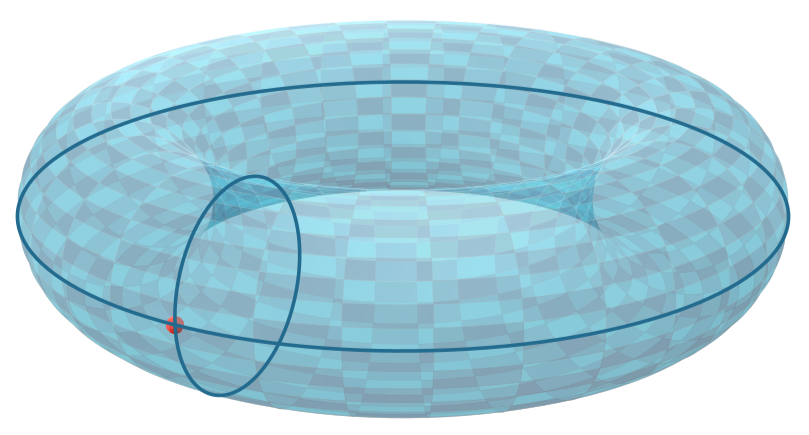
\includegraphics[width=0.5\linewidth]{pictures/ToreCW.png}
    \caption{Structure cellulaire du tore}
    \label{fig:tore-cw}
\end{figure}
\end{exemple}

Nous pouvons passer à la généralisation de construction de complexes cellulaires.

\begin{definition}
Un espace $X$ est appelé \emph{complexe cellulaire} s'il existe une structure par induction définie comme suit de $X$.

On commence avec un ensemble discret $X^0$, des points, que l'on appelle 0-cellules.

On forme par induction le \emph{n-skellettes} $X^n$ par rapport à $X^{n-1}$ en attachant chaque $n$-cellules~$e^n_\alpha$ à partir d'une application $\phi_\alpha:\s{n-1}\to X^{n-1}$. Formellement, $X^n$ est l'espace quotient de l'union disjointe $X^{n-1}\sqcup_\alpha D^n_\alpha$, de $X^{n-1}$ avec une collection de $n$-disques $D^n_\alpha$ sous l'identification $x\sim \phi_\alpha(x)$ pour $x\in\partial D_\alpha^n$. En tant qu'ensemble, on peut voir $X^n=X^{n-1}\sqcup_\alpha e^n_\alpha$ avec $e_\alpha^n$ un $n$-disque ouvert.
\end{definition}

Intuitivement, on attache chaque $(n-1)$-cellules avec une $n$-cellule. Avec l'exemple du tore, la 2-cellule permet de rattacher les deux cercles.

\begin{exemple}
Les complexes cellulaires peuvent être définis de manière intrinsèque avec le polygone fondamental. Dans cette configuration, les sommets sont des~0-cellules, les arêtes des 1-cellules, les faces des 2-cellules, et ainsi de suite. Ainsi, le ruban de Möbius et le plan projectif réel sont des complexes cellulaires. Nous pouvons aussi généraliser ceci à des polygones qui ne sont pas représentable en~2 ou 3 dimensions. Nous pouvons notamment citer le tore à $n$ dimensions, les espaces projectifs réels, et les espaces projectifs complexes.
\end{exemple}

\subsection{Le degré}

Une application $f:\s{n}\to \s{n}$ induit un morphisme sur les groupes d'homologies. Sachant que seul le $n$-ième groupe d'homologie est non trivial et isomorphe à $\bb{Z}$, nous nous intéressons alors à celui-ci.

\begin{proposition}
Un morphisme $\bb{Z}\to\bb{Z}$ est donné par $1\mapsto d$, pour $d$ un entier.
\end{proposition}
\begin{proof}
Soit $\varphi:\bb{Z}\to\bb{Z}$ un morphisme. Notons $d$ l'image de $1$ par $\varphi$. Pour $m\in \bb{Z}$, nous avons $\varphi(m)=m\varphi(1)=dm$.
\end{proof}

\begin{definition}
Pour une application $f:\s{n}\to\s{n}$, on appelle \emph{degré} de $f$ l'entier~$f_\ast(1)$, pour le morphisme induit de $\bb{Z}$ dans lui-même. Nous le noterons $\deg f$.
\end{definition}

\subsubsection{Les degrés des principales applications}

Étant donné que l'homologie est un foncteur covariant, nous pouvons directement en déduire que le degré de l'identité est 1, et que le degré d'une composition est le produit des degrés. Autrement dit, pour $\begin{tikzcd}
X\arrow[r,"g"]&Y\arrow[r,"f"]&Z,
\end{tikzcd}$ nous avons $\deg(fg)=\deg f\deg g$.

Ainsi, nous pouvons en déduire qu'une réflexion par rapport à une coordonnée a pour degré~$-1$, puisque si l'on compose deux fois une même réflexion, nous retombons sur l'identité. Ainsi, l'application antipodale sur $\s{n}$, étant une composition de réflexions sur chaque coordonnée, a pour degré~$(-1)^{n+1}$.

Pour $f\simeq g:\s{n}\to\s{n}$, nous avons $f_\ast=g_\ast$, donc $\deg f=\deg g$. La réciproque est également vraie, mais demande plus de travail.

\begin{proposition}\label{prop:deg-fixed-point}
Pour $f:\s{n}\to\s{n}$ une application sans point fixe (ie. $f(x)\neq x$ pour tout~${x\in\s{n}}$), son degré vaut $(-1)^{n+1}$.
\end{proposition}
\begin{proof}
L'application $F(t,x)=\frac{(1-t)f(x)-tx}{|(1-t)f(x)-tx|}$ est une homotopie allant de $f$ vers l'application antipodale. A noter que l'application ne passe pas par l'origine, pour tout $x\neq f(x)$.
\end{proof}

\begin{proposition}
Si $f:\s{n}\to\s{n}$ n'est pas surjective, alors $\deg f=0$.
\end{proposition}
\begin{proof}
On choisit un point $x_0\in \s{n}\setminus f(\s{n})$. Nous pouvons alors voir $f$ comme la composition $\s{n}\to\s{n}\setminus\{x_0\}\to\s{n}$. Comme $\s{n}\setminus\{x_0\}$ est contractible, son groupe d'homologie $H_n(\s{n}\setminus\{x_0\})$ est trivial. Il s'en suit alors que $f_\ast=0$.
\end{proof}

\subsubsection{Théorème de Brouwer}

Le théorème de Brouwer est un grand résultat de topologie algébrique, faisant parti des théorème du point fixe. La preuve originale de Brouwer utilise le degré pour sa démonstration.

\begin{theorem}
Toute application $f:D^n\to D^n$ admet un point fixe.
\end{theorem}
\begin{proof}
On considère deux applications $\Phi:\s{n}\to D^n,(x_0,...,x_n)\mapsto(x_0,...,x_{n-1})$, ainsi que~${\psi:D^n\to(\s{n})^+,(x_0,...,x_{n-1})\mapsto \Big(x_0,...,x_{n-1},\sqrt{1-\sum_{i=0}^{n-1}(x_i)^2}\Big)}$. Nous pouvons dès lors définir l'application~${g=\psi f\Phi:\s{n}\to \s{n}}$, qui envoie les deux hémisphères sur l'hémisphère nord, à cause de~$\psi$. Cette application est en particulier non surjective, donc de degré 0. 

D'après \ref{prop:deg-fixed-point}, une application sans point fixe est de degré $(-1)^{n+1}$. Par contraposée, notre application $g$ admet un point fixe, puisque son degré est différent de $(-1)^{n+1}$. Il existe alors $p\in \s{n}$ tel que $g(p)=\psi f\Phi(p)=p$. Or, l'application $\psi$ est bijective, ce qui nous donne $f\Phi(p)=\psi\inv(p)$. De plus, nous avons $\psi\inv(p)=\Phi(p):=q$. Nous en déduisons alors que $f(q)=q$, ce qui en fait un point fixe de $f$.
\end{proof}

\subsubsection{Degré local : la solution}

La grande question que nous nous posons actuellement, et de savoir comment nous calculons le degré concrètement, à partir d'une application quelconque. Car oui, les applications sur les sphères ne sont pas toutes homotopes à des applications connues, ou sans point fixe. Comme pour beaucoup d'autres aspects de la topologie, la réponse se trouve lorsque l'on procède localement.

Supposons que notre application $f:\s{n}\to \s{n}$ possède la propriété que des points $y\in\s{n}$ vérifie~$|f\inv(y)|<\infty$. Notons $x_0,...,x_m$ les élément de la préimage, et $U_0,...U_m$ des voisinages disjoints de chacun des points correspondant, tel que leur image est inclut dans $V\in\vois(y)$. Nous avons alors $f(U_i\setminus\{x_i\}\subset V\setminus\{y\}$ pour tout $i$, permettant de faire commuter le diagramme suivant :\[\begin{tikzcd}
&H_n(U_i,U_i\setminus\{x_i\})\arrow[r,"f_\ast"]\arrow[d,"k_i"]&H_n(V,V\setminus\{y\})\arrow[d,"\cong"]\\
H_n(\s{n},\s{n}\setminus\{x_i\})\arrow[ur, "\cong"]\arrow[dr,"\cong"]&H_n(\s{n},\s{n}\setminus\{f\inv(y)\})\arrow[l,"p_i"]\arrow[r,"f_\ast"]&H_n(\s{n},\s{n}\setminus\{y\})\\
&H_n(\s{n})\arrow[u,"q"]\arrow[r,"f_\ast"]&H_n(\s{n}).\arrow[u,"\cong"]
\end{tikzcd}\]Toutes les applications sont celles qui semblent évidentes. Les applications $p_i$ et $k_i$ sont induit des inclusions, et $q$ induit par le quotient. Les isomorphismes de la partie supérieur proviennent du théorème d'excision, tandis que ceux du bas  proviennent des séquences exactes associées. Ainsi, les deux morphismes peuvent être identifiés avec $H_n(\s{n})\cong \bb{Z}$, faisant du morphisme induit $f_\ast$ en haut un morphisme de $\bb{Z}$ dans lui même. C'est le degré de ce morphisme que nous appellerons \emph{degré local} de $f$ en $x_i$, noté $\deg f|_{x_i}$. Il s'en suit la proposition suivante, dont je vous renvoie vers \cite{Hatcher} page 136 pour une démonstration.

\begin{proposition}
Avec les mêmes notations, $\deg f=\sum_i\deg f|_{x_i}$.
\end{proposition}

\begin{exemple}
En considérant le cercle $\s{1}$ dans le plan complexe, l'application $f:z\mapsto z^k$ est de degré~$k$. Cela ce démontre par récurrence. Pour $k=0$, c'est évident car elle est non surjective. Le cas~$k<0$ s'obtient directement après avoir montré le cas $k>0$, avec la composition $z\mapsto z\inv$. Calculons alors le degré lorsque $k>0$.

Pour $y\in\s{n}$, remarquons tout d'abord que $f\inv(y)=\{x_1,...,x_k\}$, et que pour chaque point $x_i$, l'application $f$ est un homéomorphisme local. Proche de chaque $x_i$, l'application $f$ est homotope à une restriction de rotation, en étirant d'un facteur $k$ sans changer le degré local. Étant donné qu'une rotation est homotope à l'identité et un homéomorphisme, il s'en suit que le degré local de $f$ est $+1$ pour chacun des $x_i$. On en conclut que $\deg f=\sum_{i=1}^k\deg f|_{x_i}=k$.
\end{exemple}

\begin{figure}[H]
\centering
\begin{tikzpicture}
\draw[] (0,0) circle(2);
\draw[] (-2.5, 0)--(2.5,0);
\draw[] (0,-2.5)--(0,2.5);
\filldraw[](0,2) circle(1pt) node[above right]{$y$};
\filldraw[](0,-2) circle(1pt) node[below left]{$x_3$};
\filldraw[]({sqrt(3)},1) circle(1pt) node[right]{$x_1$};
\filldraw[]({-sqrt(3)},1) circle(1pt) node[left]{$x_2$};
\draw[thick, red] ({sqrt(3)},1) arc[start angle=30, end angle=40, radius=2];
\draw[thick, red] ({sqrt(3)},1) arc[start angle=30, end angle=20, radius=2]node[near start, left]{$U_1$};
\draw[thick, blue] (0,2) arc[start angle=90, end angle=120, radius=2]node[near start, below]{$f(U_1)$};
\draw[thick, blue] (0,2) arc[start angle=90, end angle=60, radius=2];
\end{tikzpicture}
\caption{Représentation du cas $k=3$ et $y=i$}
\label{fig:deg-loc-circle}
\end{figure}

\subsection{Homologie cellulaire}

La définition de l'homologie cellulaire provient du lemme qui suit. Nous nous intéresserons ci seulement au cas où $X$ est de dimension finie, qui est la dimension la plus grande de la cellule utilisée dans sa structure.

\begin{lemma}\label{lemma:cell-homology}
Si $X$ est un complexe cellulaire, alors : \begin{enumerate}[label=(\alph*)]
    \item $H_k(X^n,X^{n-1})$ vaut 0 si $k\neq n$ et est un groupe libre abélien si $k=n$, avec comme base les~$n$-cellules de $X$ ;
    \item $H_k(X^n)=0$ pour $k>n$, et en particulier, alors $H_k(X)=0$ pour~$k>\dim X$ ;
    \item L'inclusion $i:X^n\hookrightarrow X$ induit un isomorphisme si $k<n$.
\end{enumerate}
\end{lemma}
\begin{proof}
Le premier résultat provient du même raisonnement utilisé pour l'homologie simpliciale relative. Pour les autres points, on considère la séquence exacte longue de la paire $(X^n,X^{n-1})$ : \[\begin{tikzcd}
H_{k+1}(X^n,X^{n-1})\arrow[r]&H_k(X^{n-1})\arrow[r]&H_k(X^n)\arrow[r]&H_k(X^n,X^{n-1}).
\end{tikzcd}\]Si $k$ est différent de $n$ et $n-1$, alors nous avons un isomorphisme au centre. En particulier, pour~$k>n$, nous pouvons procéder par récurrence afin d'obtenir $H_k(X^n)\cong H_k(X^0)=0$. Pour $k<n$, nous avons~$H_k(X^n)\cong H_k(X^{n+m})$ par récurrence, pour tout $m>0$, montrons ainsi le dernier point pour $X$ de dimension finie.
\end{proof}

Avec ce lemme, nous pouvons construire le diagramme suivant, composé de différentes séquences exactes.

\scalebox{0.7}{
\begin{tikzcd}
&&&&0&&\\
&0\arrow[dr]&&H_n(X^{n+1})\cong H_n(X)\arrow[ur]&&&\\
&&H_n(X^n)\arrow[ur]\arrow[dr,"q_n"]&&&&\\
\cdots\arrow[r]&H_{n+1}(X^{n+1},X^n)\arrow[ur,"\partial_{n+1}"]\arrow[rr,"d_{n+1}"]&&H_n(X^n,X^{n-1})\arrow[dr,"\partial_n"]\arrow[rr,"d_n"]&&H_{n-1}(X^{n-1},X^{n-2})\arrow[r]&\cdots\\
&&&&H_{n-1}(X^{n-1})\arrow[ur,"q_{n-1}"]&&\\
&&&0\arrow[ur]&&&
\end{tikzcd}
}


Les applications $d_{n+1}$ et $d_n$ sont simplement définies comme étant les compositions respectives~$q_n\partial_{n+1}$ et $q_{n-1}\partial_n$, que l'on peut voir intuitivement comme une relativisation de l'application bordure. La composition vérifie encore $d_nd_{n+1}=0$, si bien que la ligne horizontale du diagramme définisse le \emph{complexe de chaîne cellulaire} de $X$. En effet, nous pouvons voir avec le premier point du lemme~\ref{lemma:cell-homology}, que les groupes $H_n(X^n,X^{n-1})$ sont composés des combinaisons linéaires des $n$-cellules de $X$. Les groupes d'homologies de ce complexe de chaîne cellulaire sont appelés les \emph{groupes d'homologies cellulaires} de $X$.

\begin{theorem}
Les groupes d'homologies cellulaires et les groupes d'homologies singulières sont isomorphes.
\end{theorem}
\begin{proof}
En reprenant le diagramme ci-dessus, nous pouvons remarquer l'identification de l'homologie singulière~$H_n(X)$ avec~$H_n(X^n)/\im\partial_{n+1}$, du à l'exactitude de la séquence. Le groupe~$H_n(X^n)$ a pour base les $n$-cellules de~$X$ auquel on identifies celles qui sont connectés entre elles. Cela fait alors de $j_n$ une application injective, de telle sorte que $\im\partial_{n+1}$ est isomorphe à $\im(j_n\partial_{n+1})=\im d_{n+1}$, et $H_n(X^n)$ isomorphe à $\im j_n=\ker\partial_n$. De même, $j_{n-1}$ est injectif, ce qui implique donc $\ker d_n=\ker j_{n-1}\partial_n=\ker\partial_n$. Ainsi, $j_n$ induit un isomorphisme entre le quotient $H_n(X^n)/\partial_{n+1}$ et $\ker d_n/\im d_{n+1}$. Par extension, cela démontre que $H_n(X)\cong \ker d_n/\im d_{n+1}$.
\end{proof}

\subsubsection{Et le degré ?}

En pratique, les applications $d_n$ peuvent être calculés avec le degré. Pour $n=1$, cela revient au même de calculer l'homologie simpliciale $\Delta_1(X)\to\Delta_0(X)$, et $d_1:H_1(X^1,X^0)\to H_0(X^0)$. Nous remarquerons d'ailleurs, que lorsque $X$ est connexe et ne possède qu'une seule 0-cellule (comme la figure \ref{fig:tore-cw}), alors $d_1=0$, car dans le cas contraire $H_0(X)$ ne peut être $\bb{Z}$.

\bigskip Pour une cellule $e_i^n\in X^n$, on détermine son image par $d_n$ avec la formule : \[d_n(e_i^n)=\sum_{j}d_{ij}e_j^{n-1},\]où ${d_ij}$ détermine le degré de la composition $q_j\varphi_i:\s{n-1}_i\to X^{n-1}\to\s{n-1}_j$, la composition de la fonction d'attachement $\varphi_i$ de $e^n_i$, ainsi que le quotient $q_j$, restreignant $X^{n-1}\setminus\{e^{n-1}_j\}$ à un point. 

Nous pouvons remarquer que la somme de la formule est finie, étant donné que l'image de la fonction d'attachement de $e_i^n$ est compacte, et donc qu'elle rencontre un nombre fini de cellule $e_j^{n-1}$.

\subsection{Quelques exemples}

Dans cette section, nous allons pouvoir donner quelques exemples de calculs de degrés, afin de concrétiser tous ce que nous venons de voir.

\begin{exemple}
Nous avons vu que le tore en 2 dimensions pouvait se structurer à partir d'une 0-cellule, de deux 1-cellules $\{a,b\}$, et d'une 2-cellule $T$. Cette dernière est attachée par le mot $aba\inv b\inv$, ce qui est le commutateur $[a,b]$. Nous avons alors ce complexe de chaînes cellulaire : \[\begin{tikzcd}
0\arrow[r]&\bb{Z}\arrow[r,"d_2"]&\bb{Z}^2\arrow[r,"d_1"]&\bb{Z}\arrow[r]&0.
\end{tikzcd}\] Étant donné que notre espace est connexe et est décomposé avec une seule 0-cellule, il s'en suit que~$d_1=0$. Pour le calcul de $d_2$, nous procédons ainsi.

Le degré $d_2(T)$ est donné par la somme de $d_{Ta}+d_{Tb}$. La fonction d'attachement de $T$ est~${aba\inv b\inv}$. Or, pour le calcul du degré avec $a$, le quotient $q_a$ considère la cellule $b$ comme chemin constant $c$, donnant ainsi $aca\inv c\inv\simeq c$. Autrement dit, nous avons $d_{Ta}=0$. Nous pouvons procéder de même avec $b$, donnant également $d_{T,b}=0$.

Nous pouvons en conclure que $d_2=0$, ce qui nous donne alors les groupes d'homologies suivants : \[H_k(T^2)= \left\{\begin{matrix}
\bb{Z} &k=0,2  \\
\bb{Z}^2 &k=1.  \\
\end{matrix}\right.\]
\end{exemple}
\begin{exemple}
Nous pouvons généraliser le résultat précédent pour le tore de dimension 2 avec $n$ trous, noté $T^2_n$. Il peut être décomposé en une 0-cellule, en $2n$ 1-cellules, que nous noterons $a_i,b_i$ pour $i$ de 1 à $n$, et une 2-cellule $T$, ayant comme fonction de rattachement le produit des commutateurs~${[a_1,b_1]\cdots[a_n,b_n]}$. Le complexe de chaîne cellulaire est donc le suivant : \[\begin{tikzcd}
0\arrow[r]&\bb{Z}\arrow[r,"d_2"]&\bb{Z}^{2n}\arrow[r,"d_1"]&\bb{Z}\arrow[r]&0.
\end{tikzcd}\]
De même que pour le tore, nous avons $d_1=0$. Pour le calcul de $d_2$, nous pouvons remarquer que le quotient $q_{a_i}$ envoie le produit des commutateurs, sur un lacet homotopiquement constant. Par exemple $q_{a_1}$ envoie $a_1b_1a_1\inv b_1\inv\cdots a_nb_na_n\inv b_n\inv$ sur $a_1ca_1\inv c...cccc\simeq c$. Il en est de même pour $b_i$, si bien que l'on puisse conclure que $d_2=0$. Nous obtenons alors les groupes d'homologies cellulaires suivants : 
\[H_k(T^2_{n})= \left\{\begin{matrix}
\bb{Z} &k=0,2  \\
\bb{Z}^{2n} &k=1.  \\
\end{matrix}\right.\]
\end{exemple}

\begin{wrapfigure}{l}{0.35\textwidth}
\centering
\begin{tikzpicture}[scale=.6]
% fond gris
\fill[gray!30] (0,0)--(4,0)--(5.5,1)--(5.5,5)--(1.5,5)--(0,4)--cycle;
\begin{scope}[thick,decoration={markings, mark=at position 0.5 with {\arrow{stealth}}}] 
    \draw[postaction={decorate}, red] (0,4)--(4,4)node[midway, below] {$a$};
    \draw[postaction={decorate}, red] (0,0)--(4,0) node[midway, above] {$a$};
    \draw[postaction={decorate}, dashed, red] (1.5,1)--(5.5,1) node[midway, above] {$a$};
    \draw[postaction={decorate}, red] (1.5,5)--(5.5,5) node[midway, below] {$a$};
    \draw[postaction={decorate}, blue] (0,0)--(0,4) node[midway, right] {$b$};
    \draw[postaction={decorate}, blue] (4,0)--(4,4) node[midway, left] {$b$};
    \draw[postaction={decorate},dashed, blue] (1.5,1)--(1.5,5) node[midway, left] {$b$};
    \draw[postaction={decorate}, blue] (5.5,1)--(5.5,5) node[midway, left] {$b$};
    \draw[postaction={decorate}, brown] (4,0) -- (5.5,1)node[midway, below]{$c$};
    \draw[postaction={decorate}, brown] (4,4) -- (5.5,5)node[midway, below]{$c$};
    \draw[postaction={decorate}, brown] (0,4) -- (1.5,5)node[midway, above]{$c$};
    \draw[postaction={decorate}, dashed, brown] (0,0) -- (1.5,1)node[midway, above]{$c$};
\end{scope}
%\filldraw[gray] (4.5, 2.5) circle(0)node[]{$A$};
%\filldraw[gray] (2.5, .5) circle(0)node[]{$B$};
%\filldraw[gray] (2.5, 2.5) circle(0)node[]{$C$};
\end{tikzpicture}
\caption{\centering Polygone fondamental du tore à trois dimensions}
\label{tkz:3-torus-cw}
\end{wrapfigure}

\phantom{}

\begin{exemple}
Nous passons à un exemple d'espace avec son polygone fondamental représenté en cube : le tore à 3 dimensions~${T^3=\s{1}\times\s{1}\times\s{1}}$. Sa structure de complexe cellulaire peut être donnée par une 0-cellule $v$, trois 1-cellules $a,b,c$ et trois 2-cellules~$A,B,C$ (le lettre correspondant à celle de la 1-cellule qui n'est pas dans la fonction d'attachement, comme~$A$ attaché par~$bcb\inv c\inv$), et une 3-cellule $T$ attachée par~${ABCA\inv B\inv C\inv}$. Nous obtenons alors le complexe de chaîne cellulaire suivant : \[\begin{tikzcd}
0\arrow[r]&\bb{Z}\arrow[r,"d_3"]&\bb{Z}^3\arrow[r,"d_2"]&\bb{Z}^3\arrow[r,"d_1"]&\bb{Z}\arrow[r]&0.
\end{tikzcd}\] Or, nous pouvons dans un premier temps remarquer que les 2-cellules de $T^3$ sont des tores de dimensions 2. Nous pouvons alors en déduire que l'on a $d_2=0$, ainsi que $d_1=0$. Pour $d_3$, nous allons montrer qu'il est aussi trivial. Pour cela, nous allons calculer le degré par rapport à la 2-cellule $A$. La fonction $q_A\varphi_T:\s{2}\to\s{2}$ envoie les faces $B$ et $C$ sur un point et l'intérieur de $A$ homéomorphiquement sur le complémentaire de celui-ci. Nous pourrons alors constaté que les degrés locaux des points centrés des deux faces valent respectivement 1 et $-1$, du fait que la face supérieure soit envoyé homotopiquement à l'identité, et la face inférieur corresponde à une réflexion. Son degré est alors nul, puisque la somme des degrés locaux fait 0. En procédant de même pour les autres faces, nous obtenons finalement que $d_3=0$. Nous pouvons ainsi en conclure le calcul des groupes d'homologies suivants : \[H_k(T^3)=\left\{\begin{matrix}
\bb{Z}&\text{si }k=0,3\\
\bb{Z}^3&\text{si }k=1,2.
\end{matrix}\right.\]
\end{exemple}

\begin{exemple}
Un espace projectif de dimension $n$ se construit par induction. On part d'une 0-cellule, et pour chaque $k\leq n$ le $k$-squelette est constitué d'une cellule $e^k$, que l'on attache à la $k-1$-cellule par la projection du revêtement à deux feuillets de la sphère de dimension $k$, c'est à dire~${\varphi:\s{k-1}\to\realproj^{k-1}}$. Avec cette construction, nous pouvons comprendre que le $k$-squelette correspond à l'espace projectif~$\realproj^k$. Le calcul du morphisme $d_k$ revient à calculer le degré de la composition~${\s{k-1}\to \realproj^{k-1}\to\realproj^{k-1}/\realproj^{k-2}=\s{k-1}}$, de la fonction d'attachement $\varphi$ et du quotient de squelette $X^k/X^{k-1}$. Restreinte à chaque hémisphère de $\s{k-1}\setminus\s{k-2}$, la composition est composée de deux homéomorphismes, qui sont antipodales l'une de l'autre. Il s'en suit que les degré sont inversibles, et donc valent $-1$ ou $1$. On en conclut alors que le degré peut être obtenu par~${d_k=\deg id+\deg (-id)=1+(-1)^k}$. Le degré est donc alternativement 0 pour $k$ impair, et $2$ pour~$k$ pair. Cela nous donne les suites de morphismes suivantes : \[\begin{tikzcd}
    0\arrow[r]&\bb{Z}\arrow[r,"2"]&\bb{Z}\arrow[r,"0"]&\bb{Z}\arrow[r,"2"]&\cdots\arrow[r,"0"]&\bb{Z}\arrow[r,"2"]&\bb{Z}\arrow[r,"0"]&0.\text{ si $n$ est pair,}
\end{tikzcd}\]
et
\[\begin{tikzcd}
    0\arrow[r]&\bb{Z}\arrow[r,"0"]&\bb{Z}\arrow[r,"2"]&\bb{Z}\arrow[r,"0"]&\cdots\arrow[r,"0"]&\bb{Z}\arrow[r,"2"]&\bb{Z}\arrow[r,"0"]&0.\text{ si $n$ est impair.}
\end{tikzcd}\]Lors des calculs d'homologies, nous nous retrouvons alors avec $\ker d_k/2\im d_{k+1}$, ce qui nous donne le résultat suivant : \[H_k(\realproj^n)=\left\{\begin{matrix}
\bb{Z}&si\ k=0,\ et\ k=n\text{ si n impair}\\
\bb{Z}_2&si\  k\ impair,\,0<k<n\\
0&sinon.
\end{matrix}\right.\]
\end{exemple}

\begin{exemple}
L'espace projectif complexe de dimension $n$, noté $\compproj^n$, est défini comme étant l'ensemble des droites vectorielles de l'espace complexe $\bb{C}^{n+1}$. Topologiquement, il est construit de manière inductive avec une cellule toute les dimensions paires jusqu'à $2n$. Cela donne donc une séquence de groupe alternativement trivial et isomorphe à $\bb{Z}$. On en déduit donc que les morphismes $d_k$ sont tous triviaux, ce qui fait que l'on obtient les groupes d'homologies suivants : \[H_k(\compproj^n)=\left\{\begin{matrix}
\bb{Z}&si\ k\ pair\\
0&sinon.
\end{matrix}\right.\]
\end{exemple}

\subsubsection{Autres résultats de l'homologie cellulaire}

Le résultat qui nous a permis de conclure si rapidement pour l'exemple de l'espace projectif complexe est plus générique que ça.

\begin{proposition}
Si les cellules d'un complexe cellulaire $X$ n'ont pas de dimensions adjacentes, alors les groupes d'homologies $H_k(X)$ ont une base en correspondance une par une avec les $k$-cellules de $X$.
\end{proposition}
\begin{proof}
Dans ce cas, les morphismes $d_k$ sont tous triviaux.
\end{proof}

Il existe d'autres résultats intéressant permettant de simplifier les calculs d'homologies. 

\begin{proposition}
Si un complexe cellulaire $X$ ne possède pas de $n$-cellule, alors $H_n(X)=0$.
\end{proposition}
De manière plus générale, nous avons aussi le résultat qui suit.
\begin{proposition}
Si $X$ est un complexe cellulaire avec $k$ $n$-cellules, alors $H_n(X)$ est généré par au plus $k$ éléments.
\end{proposition}
\begin{proof}
Avec les mêmes notations, cela vient du fait que $H_n(X^n,X^{n-1})$ est un groupe libre avec $k$ générateurs. Ainsi, le sous-groupe $\ker d_n$ possède un maximum de $k$ générateurs, ce qui vaut également pour le quotient $\ker d_n/\im d_{n+1}$.
\end{proof}

\appendix
\chapter{Calculs avec l'homologie simpliciale}\label{chap:annexe-simp-homo}

Dans cette première annexe, nous allons voir comment nous utilisons l'homologie simpliciale en pratique. Nous avons déjà traiter l'exemple du cercle dans la section \ref{sect:simpl-homology}. Nous nous intéresserons dans un premier temps aux espaces formé d'un polygone fondamental carré : le tore de dimension 2, le plan projectif réel, la bouteile de Klein, le ruban de Möbius. Par la suite, nous intéresserons au calcul de la sphère de dimensions 2. Après cela, nous montrerons avec l'exemple du tore à 2 trous et de la sphère de dimension quelconque que cet outils de calcul devient vite exhaustif pour des espaces plus compliqués.

\section{Polygones fondamentaux}

\subsection{C'est carré !}

\begin{figure}[H]
\centering
\begin{subfigure}[b]{0.45\textwidth}
\centering
\begin{tikzpicture}[scale=.6]
% fond gris
\fill[gray!30] (0,0) -- (4,0) -- (0,4) -- cycle;
\fill[gray!30] (6,4) -- (6,0) -- (2,4) -- cycle;
\begin{scope}[thick,decoration={markings, mark=at position 0.5 with {\arrow{stealth}}}] 
    %A
    \draw[postaction={decorate}, red] (0,0)--(4,0) node[midway, above] {$a_1$};
    \draw[postaction={decorate}, blue] (0,0)--(0,4) node[midway, right] {$b_1$};
    \draw[postaction={decorate}, brown] (4,0) -- (0,4)node[midway, below]{$c_1$};
    %B
    \draw[postaction={decorate}, red] (2,4)--(6,4)node[midway, below] {$a_2$};
    \draw[postaction={decorate}, blue] (6,0)--(6,4) node[midway, left] {$b_2$};
    \draw[postaction={decorate}, brown] (6,0) -- (2,4)node[midway, above]{$c_2$};
\end{scope}
    \filldraw[] (6,0) circle(1pt) node[right]{$v_0'$};
    \filldraw[] (4,0) circle(1pt) node[above]{$v_1$};
    \filldraw[] (0,4) circle(1pt) node[left]{$v_2$};
    \filldraw[] (2,4) circle(1pt) node[above right]{$v_1'$};
    \filldraw[] (6,4) circle(1pt) node[right]{$v_2'$};
    \filldraw[] (0,0) circle(1pt) node[left]{$v_0$};
    \filldraw[gray] (1,1) circle(0pt) node[]{$A$};
    \filldraw[gray] (5,3) circle(0pt) node[]{$B$};
\end{tikzpicture}
\caption{\centering Structure simpliciale sans identifications}
\label{tkz:simplicial-torus-before}
\end{subfigure}
\begin{subfigure}[b]{0.45\textwidth}
\centering
\begin{tikzpicture}[scale=.6]
% fond gris
\fill[gray!30] (0,0) rectangle (4,4);
\begin{scope}[thick,decoration={markings, mark=at position 0.5 with {\arrow{stealth}}}] 
    \draw[postaction={decorate}, red] (0,4)--(4,4)node[midway, below] {$a$};
    \draw[postaction={decorate}, red] (0,0)--(4,0) node[midway, above] {$a$};
    \draw[postaction={decorate}, blue] (0,0)--(0,4) node[midway, right] {$b$};
    \draw[postaction={decorate}, blue] (4,0)--(4,4) node[midway, left] {$b$};
    \draw[postaction={decorate}, brown] (4,0) -- (0,4)node[midway, below]{$c$};
\end{scope}
    \filldraw[] (4,0) circle(1pt) node[right]{$v$};
    \filldraw[] (0,4) circle(1pt) node[left]{$v$};
    \filldraw[] (4,4) circle(1pt) node[right]{$v$};
    \filldraw[] (0,0) circle(1pt) node[left]{$v$};
    \filldraw[gray] (1,1) circle(0pt) node[]{$A$};
    \filldraw[gray] (3,3) circle(0pt) node[]{$B$};
\end{tikzpicture}
\caption{\centering Structure simpliciale du tore}
\label{tkz:simplicial-torus}
\end{subfigure}
\end{figure}

\phantom{}

\begin{exemple}
Nous commençons par le tore de dimension 2, que l'on appellera tore, et notera $T^2$. Nous reprenons la structure simpliciale que nous avons proposé dans la section \ref{sect:simplices}. A partir des deux 2-simplexes $A=[v_0,v_1,v_2]$ et $B=[v_0',v_1',v_2']$ (voir figure \ref{tkz:simplicial-torus-before}), nous avons procédé à plusieurs identifications sur les sommets et les côtés afin d'aboutir à la structure simpliciale du tore \ref{tkz:simplicial-torus}. Voici un exemple d'identifications effectués : \begin{itemize}
    \item Sur les sommets, tout les points sont identifiés entre eux, ne faisant qu'un, noté $v$ ;
    \item Sur les côtés : $a_1\approx a_2$, $b_1\approx b_2$ et $c_1\approx c_2$, leurs identifications sont notés respectivement~$a,b,c$.
\end{itemize}
Nous avons alors la chaîne de complexes simpliciaux suivante : \[\begin{tikzcd}
\Delta_2(T^2)=\langle A,B\rangle\cong\bb{Z}^2\arrow[r]&\Delta_1(T^2)=\langle a,b,c\rangle\cong\bb{Z}^3\arrow[r]&\Delta_0(T^2)=\langle v\rangle\cong\bb{Z}.
\end{tikzcd}\]Nous pouvons ainsi procédé aux calculs des bordures. Pour cela, deux méthodes similaires sont possibles. La première étant de considérer les identifications établis, la deuxième étant de voir les identifications ensuite, et d'appliquer la formule de la bordure automatiquement.

Pour la première méthode, on considère que le sens de rotation est trigonométrique (le signe du simplexe tournant dans ce sens est positif, sinon négatif), de telle sorte que l'on ait les bordures~$\partial_2(A)=c-b+a$ et~${\partial_2(B)=-c+b-a}$. Comme les 1-simplexes ont le même point au départ et à l'arrivée, on a~${\partial_1(a)=\partial_1(b)=\partial_1(c)=v-v=0}$. Enfin, nous avons $\partial_0(v)=0$.

\bigskip Pour le calcul de l'homologie, nous pouvons commencer par voir que $\im\partial_3=0$. En remarquant que $\partial_2(A)=-\partial_2(B)$, nous avons ${\partial_2(A-B)=\partial_2(A)-\partial_2(B)=0}$, ce qui nous permet d'obtenir~${\ker\partial_2=\langle A-B\rangle}$. Ainsi, le groupe d'homologie $\homsimp_2(T^2)=\ker\partial_2/\im\partial_3=\langle A-B\rangle\cong \bb{Z}$. 

Pour le seconde groupe, nous pouvons dans un premier temps voir $\im\partial_2=\langle a-b+c\rangle$, ainsi que~$\ker\partial_1=\langle a,b,c\rangle$. Nous obtenons alors le groupe d'homologie suivant :  $$\homsimp_2(T^2)=\langle a,b,c\rangle/\langle a-b+c\rangle=\langle a,b,c|a+c=b\rangle=\langle a,a+c,c\rangle=\langle a,c\rangle\cong \bb{Z}^2.$$

Pour le premier groupe d'homologie, il est immédiat : $\homsimp_0(T^2)=\langle v\rangle/\{0\}=\langle v\rangle\cong \bb{Z}$.

Finalement, nous obtenons la séquence de groupe d'homologies suivante : \[\begin{tikzcd}
    0\arrow[r]&\bb{Z}\arrow[r]&\bb{Z}^2\arrow[r]&\bb{Z}\arrow[r]&0.
\end{tikzcd}\]

Pour la second méthode, nous calculons les bordures de la manière suivante : \begin{itemize}
    \item Pour les 2-simplexes : $\partial_2(A)=\partial([v_0,v_1,v_2])=[v_1,v_2]-[v_0,v_2]+[v_0,v_1]=c_1-b_1+a_1$, et de même $\partial_2(B)=[v_1',v_2']-[v_0',v_2']+[v_0',v_1']=c_2-b_2+a_2$ ;
    \item Pour le simplexe $A$ : $\partial_1(a_1)=\partial([v_0,v_1])=v_1-v_0$, $\partial_1(b_1)=v_2-v_0$ et ${\partial_1(c_1)=v_2-v_1}$. Nous obtenons les résultats identiques pour le simplexe $B$ ;
    \item Pour les 0-simplexes, toutes leurs images sont nulles.
\end{itemize}
Pour le calcul du groupe d'homologie, nous procédons aux identifications énoncées, de telle sorte que nous retombons sur les résultats données plus haut.
\end{exemple}

\begin{wrapfigure}{r}{0.4\linewidth}
\centering
\begin{tikzpicture}[scale=0.8]
    % fond gris
    \fill[gray!30] (0,0) rectangle (4,4);
\begin{scope}[thick,decoration={markings, mark=at position 0.5 with {\arrow{stealth}}}] 
    \draw[postaction={decorate}, red] (0,4)--(4,4)node[midway, below] {$a$};
    \draw[postaction={decorate}, red] (4,0)--(0,0) node[midway, above] {$a$};
    \draw[postaction={decorate}, blue] (0,4)--(0,0) node[midway, right] {$b$};
    \draw[postaction={decorate}, blue] (4,0)--(4,4) node[midway, left] {$b$};
    \draw[postaction={decorate}, brown] (4,0) -- (0,4)node[midway, below]{$c$};
\end{scope}
    \filldraw[] (4,0) circle(1pt) node[right]{$v_0$};
    \filldraw[] (0,4) circle(1pt) node[left]{$v_0$};
    \filldraw[] (4,4) circle(1pt) node[right]{$v_1$};
    \filldraw[] (0,0) circle(1pt) node[left]{$v_1$};
    \filldraw[gray] (1,1) circle(0pt) node[]{$A$};
    \filldraw[gray] (3,3) circle(0pt) node[]{$B$};
\end{tikzpicture}
\caption{\centering Structure simpliciale du plan projectif réel}
\label{tkz:simplicial-proj}
\end{wrapfigure}
Nous allons par la suite ne plus donner les identifications effectués sur la structure simpliciale, elles sont semblable à celle donnée dans l'exemple précédent.

\begin{exemple}
Désormais, nous allons nous intéresser au calcul du plan projectif réel $\realproj^2$. En considérant la structure de la figure \ref{tkz:simplicial-proj}, nous avons la chaîne de complexes simpliciaux suivante : 
\[\footnotesize
\begin{tikzcd}
0\arrow[r]&\langle A,B\rangle\arrow[r]&\langle a,b,c\rangle\arrow[r]&=\langle v_0,v_1\rangle\arrow[r]&0.
\end{tikzcd}
\]

Pour les calculs des bordures, nous considérons le sens trigonométrique. Ainsi, nous avons $\partial_2(A)=c+b-a$ et~$\partial_2(B)=-c+b-a$. Ensuite, nous avons $\partial_1(a)=v_1-v_0$, ainsi que $\partial_1(b)=v_1-v_0$ et $\partial_1(c)=v_1-v_1=0$.

\bigskip Pour les calculs des groupes d'homologies, nous pouvons facilement voir qu'il n'existe pas de combinaisons linéaires des images de bordures de $A$ et $B$ donnant 0. Autrement dit nous avons l'implication~$\partial_2(\alpha A+\beta B)=0\Rightarrow \alpha=\beta=0$, permettant de dire que $\ker\partial_2=0$. Nous pouvons en déduire $\homsimp_2(\realproj^2)=0$. Nous pouvons également facilement trouver le résultat qui suit : $$\homsimp_0(\realproj^2)=\langle v_0,v_1\rangle/\langle v_1-v_0\rangle=\langle v_0,v_1|v_0=v_1\rangle\cong\bb{Z}.$$Enfin, nous avons $\im\partial_2=\langle c+b-a,c-b+a\rangle$ et $\ker\partial_1=\langle c, b-a\rangle$. Cela nous permet de calculer le groupe d'homologie suivant : \[\homsimp_1(\realproj^2)=\langle c, b-a\rangle/\langle c+b-a,c-b+a\rangle=\langle c,b-a|c=a-b,c=b-a\rangle.\]Sur la dernière égalité, nous avons $c=-c$, ce qui se traduit algébriquement par $\langle c\rangle=\bb{Z}_2$. Nous en déduisons alors que $\homsimp_1(\realproj^2)=\bb{Z}_2$.
\end{exemple}

\begin{wrapfigure}{r}{.3\textwidth}
\centering
\begin{tikzpicture}[scale=.8]
    % fond gris
    \fill[gray!30] (0,0) rectangle (4,4);
    %flèche du haut
\begin{scope}[thick,decoration={markings, mark=at position 0.5 with {\arrow{stealth}}}] 
    \draw[postaction={decorate}, red] (0,4)--(4,4)node[midway, below] {$a$};
    \draw[postaction={decorate}, red] (4,0)--(0,0) node[midway, above] {$a$};
    \draw[postaction={decorate}, blue] (0,0)--(0,4) node[midway, right] {$b$};
    \draw[postaction={decorate}, blue] (4,0)--(4,4) node[midway, left] {$b$};
    \draw[postaction={decorate}, brown] (4,0) -- (0,4)node[midway, below]{$c$};
\end{scope}
    \filldraw[] (4,0) circle(1pt) node[right]{$v$};
    \filldraw[] (0,4) circle(1pt) node[left]{$v$};
    \filldraw[] (4,4) circle(1pt) node[right]{$v$};
    \filldraw[] (0,0) circle(1pt) node[left]{$v$};
    \filldraw[gray] (1,1) circle(0pt) node[]{$A$};
    \filldraw[gray] (3,3) circle(0pt) node[]{$B$};
\end{tikzpicture}
\caption{\centering Structure simpliciale de la bouteille de Klein}
\label{tkz:klein-bottle-simp}
\end{wrapfigure}

\phantom{}

\begin{exemple}
Pour la bouteille de Klein, notée $K$, nous considérons la structure simpliciale proposée sur la figure \ref{tkz:klein-bottle-simp}. Nous obtenons alors le complexe de chaînes simpliciales suivant : 
\[\footnotesize
\begin{tikzcd}
0\arrow[r]&\langle A,B\rangle\arrow[r]&\langle a,b,c\rangle\arrow[r]&\langle v\rangle\arrow[r]&0.
\end{tikzcd}
\]Pour les calculs de bordures, nous avons $\partial_2(A)=c-b-a$ et~${\partial_2(B)=b-c-a}$. Également, comme il n'y a qu'un seul 0-simplexe, nous avons $\partial_1=0$.

Pour les groupes d'homologies, nous avons~${\homsimp_0(K)=\langle v\rangle\cong\bb{Z}}$. Ensuite, nous avons~${\ker\partial_2=0}$, pour la même raison que le plan projectif. Enfin, nous avons le groupe d'homologie simpliciale suivant : \[\begin{split}
\homsimp_1(K)&=\langle a,b,c|b-c-a=0,c-b-a=0\rangle\\
&=\langle a,b,c|a=b-c,a=c-b\rangle\\
&=\langle b,c|b-c=c-b\rangle\\
&=\langle b,c-b|2(c-b)=0\rangle\\
&\cong \bb{Z}\oplus\bb{Z}_2.
\end{split}\]
\end{exemple}

\begin{wrapfigure}{r}{.3\textwidth}
\centering
\begin{tikzpicture}[scale=.8]
    % fond gris
    \fill[gray!30] (0,0) rectangle (4,4);
    %flèche du haut
\begin{scope}[thick,decoration={markings, mark=at position 0.5 with {\arrow{stealth}}}] 
    \draw[postaction={decorate}, red] (0,4)--(4,4)node[midway, below] {$a$};
    \draw[postaction={decorate}, red] (4,0)--(0,0) node[midway, above] {$a$};
    \draw[postaction={decorate}] (0,0)--(0,4) node[midway, right] {$b_1$};
    \draw[postaction={decorate}] (4,0)--(4,4) node[midway, left] {$b_2$};
    \draw[postaction={decorate}, brown] (4,0) -- (0,4)node[midway, below]{$c$};
\end{scope}
    \filldraw[] (4,0) circle(1pt) node[right]{$v_0$};
    \filldraw[] (0,4) circle(1pt) node[left]{$v_0$};
    \filldraw[] (4,4) circle(1pt) node[right]{$v_1$};
    \filldraw[] (0,0) circle(1pt) node[left]{$v_1$};
    \filldraw[gray] (1,1) circle(0pt) node[]{$A$};
    \filldraw[gray] (3,3) circle(0pt) node[]{$B$};
\end{tikzpicture}
\caption{\centering Structure simpliciale du ruban de Möbius}
\label{tkz:mobius-strip-simp}
\end{wrapfigure}

\phantom{}

\begin{exemple}
Pour le ruban de Möbius $M$, nous avons les deux faces $b_1$ et $b_2$ qui ne sont pas identifiées entre elles, ce qui change par rapport aux exemples précédents. Pour la chaîne de complexe cellulaire, nous avons alors : \[\footnotesize
\begin{tikzcd}
0\arrow[r]&\langle A,B\rangle\arrow[r]&\langle a,b_1,b_2,c\rangle\arrow[r]&\langle v_0, v_1\rangle\arrow[r]&0.
\end{tikzcd}
\]Pour les calculs de bordures, nous avons d'un côté $\partial_2(A)=c-b_1-a$ et~$\partial_2(B)=-c+b_2-a$, et de l'autre $\partial_1(a)=v_1-v_0=\partial_1(b_2)$, ainsi que~$\partial_1(b_1)=v_0-v_1$ et $\partial_1(c)=0$. Nous avons toujours $\partial_0=0$.

Cela nous donne donc les résultats suivants sur les groupes d'homologies. Tout d'abord, $\homsimp_2(M)=0$ du fait que les images sont linéairement indépendantes. Ensuite, nous avons $\homsimp_0\cong\bb{Z}$ par le même calcul que pour du plan projectif. Enfin, nous avons les calculs suivants pour le groupe d'homologie $\homsimp_1$ : \[\begin{split}
\homsimp_1(M)&=\langle c,a+b_1,a-b_2\rangle/\langle c-b_1-a,c-b_2+a\rangle\\
&=\langle c,a+b_1,a-b_2|c-b_1-a=0,c-b_2+a=0\rangle\\
&=\langle c,a+b_1,a-b_2|c=b_1+a,c=b_2-a\rangle\\
&\cong \bb{Z}
\end{split}\]Vu que les trois générateurs sont "liés", ils ne forment qu'un, d'où l'isomorphisme avec $\bb{Z}$.
\end{exemple}

\newpage
\subsection{Si c'est rond}
Dans cette partie, nous allons calculer l'homologie simpliciale de la sphère $\s{2}$, que l'on appellera sphère.
\begin{figure}[H]
\centering
\begin{subfigure}[b]{.45\linewidth}
\centering
\begin{tikzpicture}[scale=.8]
\fill[gray!30] (0,0)--(4,0)--(2,3)-- cycle ;
\fill[gray!30] (4,1)--(8,1)--(6,4)-- cycle ;
\begin{scope}[thick,decoration={markings, mark=at position 0.5 with {\arrow{stealth}}}] 
    \draw[postaction={decorate}, red] (0,0)--(4,0)node[midway, above] {$e_1$};
    \draw[postaction={decorate}, blue] (4,0)--(2,3) node[midway, left] {$e_2$};
    \draw[postaction={decorate}, brown] (0,0)--(2,3) node[midway, right] {$e_3$};
    \draw[postaction={decorate}, red] (4,1)--(8,1) node[midway, below left] {$f_1$};
    \draw[postaction={decorate}, blue] (8,1) -- (6,4)node[midway, left]{$f_2$};
    \draw[postaction={decorate}, brown] (4,1)--(6,4)node[midway, right]{$f_3$};
\end{scope}
\filldraw[] (0,0) circle(1pt)node[left]{$\Tilde{v}_0$};
\filldraw[] (4,0) circle(1pt)node[right]{$\Tilde{v}_1$};
\filldraw[] (2,3) circle(1pt)node[above left]{$\Tilde{v}_2$};
\filldraw[] (4,1) circle(1pt)node[below right]{$\Tilde{w}_0$};
\filldraw[] (8,1) circle(1pt)node[right]{$\Tilde{w}_1$};
\filldraw[] (6,4) circle(1pt)node[above left]{$\Tilde{w}_2$};
\filldraw[] (2,1) circle(0pt)node[]{$T$};
\filldraw[] (6,2) circle(0pt)node[]{$B$};
\end{tikzpicture}
\caption{\centering Structure simpliciale de la sphère $\s{2}$}
\end{subfigure}
\begin{subfigure}[b]{0.45\linewidth}
\centering
\begin{tikzpicture}
\filldraw[gray!15] (0,0) circle(2);
\draw[] (0,0) circle(2);
\begin{scope}[thick,decoration={markings, mark=at position 0.5 with {\arrow{stealth}}}] 
    \draw[postaction={decorate}, red] (-2,0).. controls(-1,-.2)..(0,-.3)node[midway, below] {$a$};
    \draw[postaction={decorate}, blue] (0,-.3).. controls(1,-.2)..(2,0)node[midway, below] {$b$};
    \draw[postaction={decorate}, dashed, brown] (-2,0).. controls(0,0.4)..(2,0)node[midway, above] {$c$};
\end{scope} 
\filldraw[] (-2,0) circle(1pt) node[left]{$v_0$};
\filldraw[] (0,-.3) circle(1pt) node[below]{$v_1$};
\filldraw[] (2,0) circle(1pt) node[right]{$v_2$};
\filldraw[] (0,1) circle(0) node[right]{$T$};
\filldraw[] (0,-1) circle(0) node[right]{$B$};
\end{tikzpicture}
\caption{Sphère structuré à base de simplexes}
\label{tkz:sphere2-simp}
\end{subfigure}
\caption{La sphère $\s{2}$ et sa structure simpliciale}
\label{fig:sphere2-simp}
\end{figure}

\begin{exemple}
La structure simpliciale de la sphère que nous utilisons ici part de deux 2-simplexes $T$ et~$B$, auquel nous identifions les sommets et côtés deux à deux, avec sons correspondant dans l'ordre du simplexe. Intuitivement, le premier simplexe $T$ recouvre l'hémisphère nord et le second recouvre l'hémisphère sud, et leurs cotés forment un cercle, l'équateur. Avec les notations utilisés dans les figures ci-dessus \ref{fig:sphere2-simp}, les identifications sont données de façon implicite par les couleurs ou par leur indices.

Pour les calculs de bordures, nous avons tout d'abord $\partial_2(T)=\partial_2(B)=b-c+a$, ensuite nous avons~${\partial_1(a)=v_1-v_0}$, $\partial_1(b)=v_2-v_1,\partial_1(c)=v_2-v_0$, et enfin $\partial_0=0$. Cela nous donne donc les résultats suivants pour l'homologie :
\begin{itemize}
    \item $\homsimp_0(\s{2})=\langle v_0,v_1,v_2|v_0=v_1=v_2\rangle\cong\bb{Z}$;
    \item $\homsimp_2(\s{2})=\langle T-B\rangle\cong\bb{Z}$;
    \item Pour trouver un élément de $\ker\partial_1$, nous allons chercher à trouver une solution de l'équation~${\partial_1(\alpha a+\beta b+\gamma c)=0}$. Cela nous donne $(\beta+\gamma)v_2+(\alpha-\beta)v_1-(\alpha+\gamma)v_0=0$, en calculant l'image de la bordure. Or, il n'existe aucune combinaison donnant un tel résultat, ce qui veut donc dire que le noyau est trivial. Ainsi, nous obtenons $\homsimp_1(\s{2})=0$.
\end{itemize}
\end{exemple}


\section{Limitations de l'homologie simpliciale}
%2-tore

\begin{wrapfigure}{r}{0.3\textwidth}
\centering
\begin{tikzpicture}[scale=.6]
\fill[gray!30] (2,0)--(4,0)--(6,2)--(6,4)--(4,6)--(2,6)--(0,4)--(0,2)-- cycle ;
\begin{scope}[thick,decoration={markings, mark=at position 0.5 with {\arrow{stealth}}}] 
    \draw[postaction={decorate}, red] (2,0)--(4,0)node[midway, above] {$a$};
    \draw[postaction={decorate}, blue] (4,0)--(6,2) node[midway, above left] {$b$};
    \draw[postaction={decorate}, red] (6,4)--(6,2) node[midway, left] {$a$};
    \draw[postaction={decorate}, blue] (4,6)--(6,4) node[midway, below left] {$b$};
    \draw[postaction={decorate}, brown] (4,6) -- (2,6)node[midway, below]{$c$};
    \draw[postaction={decorate}, DarkGreen] (2,6)--(0,4)node[midway, below right]{$d$};
    \draw[postaction={decorate}, brown](0,2)--(0,4)node[midway, right]{$c$};
    \draw[postaction={decorate}, DarkGreen](2,0)--(0,2)node[midway, above right]{$d$};
    \draw[postaction={decorate}](2,0)--(6,2);
    \draw[postaction={decorate}](2,0)--(6,4);
    \draw[postaction={decorate}](2,0)--(4,6);
    \draw[postaction={decorate}](2,0)--(2,6);
    \draw[postaction={decorate}](2,0)--(0,4);
\end{scope}
\end{tikzpicture}
\caption{\centering Structure simpliciale du 2-tore}
\label{tkz:2-torus-simp}
\end{wrapfigure}

Lorsque nous nous intéressons à des espaces avec des polygones fondamentaux plus sophistiqués, tel que le 2-tore sur la figure \ref{tkz:2-torus-simp}, la structure simpliciale devient assez rapidement énorme. Dans notre cas, nous avons six 2-simplexes, treize 1-simplexes et un 0-simplexe, pour un seul trou en plus ! Nous pouvons très bien conjecturer le fait que ce nombre grandis de plus en plus en fonction du nombre de trous. Pour des espaces encore plus complexes, tel que le tore de dimension supérieure, ou bien les espace projectifs, cela semble être encore plus compliqué. C'est en ce sens que l'homologie cellulaire est plus utile en pratique, elle ne demande pas de structure aussi explicite et longue.

\bigskip En plus de cela, l'homologie simpliciale de la sphère de dimension supérieure à deux devient vite complexe (même si nous connaissons le résultat), du fait qu'il faut démontrer que les groupes d'homologies autres que 0 et la dimension de la sphère sont triviaux.
\chapter{Introduction à la théorie des catégories}\label{chap:categories}

Intuitivement, la théorie des catégories a pour but d'être une théorie très vague et globale, permettant de trouver des résultats universels. Nous nous éloignons de toutes restrictions, de tout axiomes et propriétés à vérifier, pour pouvoir englober tout types de contenant. Nous pouvons ainsi considérer les espaces topologiques de la même manière que les groupes. C'est avec cette idée de généralisation que l'on a pu construire de si bons outils de topologie algébriques. Le lecteur souhaitant plus de détails sur la théorie des catégories est invité à lire \cite{MacLane}.

\begin{definition}
Une \emph{catégorie} $\mathcal{C}$ consiste en trois choses : \begin{itemize}[label=$\bullet$]
    \item Une collection d'\emph{objets} $Ob(\mathcal{C})$ ;
    \item Pour tout couple $(X,Y)$ d'objets, les ensembles $Mor(X,Y)$ appelés \emph{morphismes}, ainsi que le morphisme \emph{identité} $id_X=id\in Mor(X,X)$ pour tout $X\in Ob(\mathcal{C})$ ;
    \item Une fonction de \emph{composition de morphismes} : $Mor(X,Y)\times Mor(Y,Z)\to Mor(X,Z)$ pour tout triplet $(X,Y,Z)\in Ob(\mathcal{C})^3$, satisfaisant l'axiome $f\circ id=id\circ f=f$, et $(f\circ g)\circ h=f\circ(g\circ h)$, pour les morphismes adéquats.
\end{itemize}
\end{definition}

Selon les auteurs, les morphismes sont également appelés flèches, et noté $f:X\to Y$ plutôt que $f\in Mor(X,Y)$.

\begin{exemple}Nous pouvons citer quelques exemples de catégories, en lien ou non avec la topologie algébrique, pour montrer à quel point cette notion peut englober de concepts mathématiques.
\begin{enumerate}
    \item Nous pouvons considérer les espaces topologiques comme une catégories. Les objets peuvent être simplement des espaces topologiques $(X,\mathcal{T})$. Les morphismes peuvent être les applications continues, ou bien l'on peut se restreindre aux homéomorphismes, ou encore aux homotopies. Dans les trois cas, les axiomes sont vérifiées et le morphisme identité existe.
    \item L'ensemble des groupes peut être une catégorie, avec les groupes comme objets et les morphismes de groupes étant des morphismes. Le sous-ensemble des groupes abéliens forme également une catégorie.

    De manière plus générale, l'ensemble des modules sur un corps fixe représentent une catégorie.
    \item Un groupe peut être vue comme une catégorie, avec un seul objet et les morphismes étant les éléments ce groupe. Nous pouvons même voir les monoïdes (magma unitaire et LCI transitive) en tant que catégories, si l'on souhaite voir plus large.
    \item Étant donné un corps $K$, l'ensemble des matrices sur $K$ forme une catégorie, avec les objets étant des entiers, et $Mor(n,m)$ l'ensemble des matrices de taille $n\times m$.
\end{enumerate}
Plein d'autres exemples de catégories sont donnés \cite{Hatcher} page 163.
\end{exemple}

\begin{definition}\label{def:functor}
Un \emph{foncteur} $F$ allant d'une catégorie $\mathcal{C}$ à une catégorie $\mathcal{D}$ envoie chaque objet~${X\in Ob(\mathcal{C})}$ un objet $F(X)\in Ob(\mathcal{D})$, ainsi que, pour tout couple $(X,Y)\in Ob(\mathcal{C})^2$, chaque morphisme $f\in Mor(X,Y)$ est envoyé vers~${F(f)\in Mor(F(X),F(Y)}$, et tel qu'il vérifie $F(id)=id$.

On dit d'un foncteur $F$ qu'il est \emph{covariant} s'il vérifie $F(f\circ g)=F(f)\circ F(g)$. S'il vérifie $F(f\circ g)=F(g)\circ F(f)$, alors on dit qu'il est \emph{contravariant}.
\end{definition}

\begin{exemple}
Le groupe fondamental est un foncteur entre la catégories des espaces pointés avec les applications continues, que l'on note $Top_\ast$, vers la catégories des groupes, noté $Grp$. De même, les groupes d'homologie sont des foncteurs entre la catégorie $Top$ des espaces topologies vers la catégories des groupes abéliens $Ab$.
\end{exemple}

\begin{wrapfigure}{r}{0.3\textwidth}
\centering
\begin{tikzcd}
F(X)\arrow[r,"F(f)"]\arrow[d,"T_X"]&F(Y)\arrow[d,"T_Y"]\\
G(X)\arrow[r,"G(f)"]&G(Y).
\end{tikzcd}
\end{wrapfigure}

Il existe un dernier concept, permettant de passer d'un foncteur à un autre.

\begin{definition}
Une \emph{transformation naturelle} $T$ entre deux foncteurs $F,G:\mathcal{C}\to\mathcal{D}$ assigne un morphisme $T_X:F(X)\to G(X)$ à chaque objet $X\in Ob(\mathcal{C})$, de telle sorte que le diagramme ci-contre commute, pour tout morphisme $f\in Mor(X,Y)$.
\end{definition}

\begin{exemple}
L'abélianisation est une transformation naturelle entre le groupe fondamental et le groupe d'homologie $H_1$.
\end{exemple}
%\chapter{Autres références}

\begin{itemize}
    \item \href{https://www.youtube.com/playlist?list=PLOROtRhtegr7DmeMyFxfKxsljAVsAn_X4}{Algebraic Topology - Math at Andrews University}
    \item \href{https://www.youtube.com/playlist?list=PLpRLWqLFLVTCL15U6N3o35g4uhMSBVA2b}{Algebraic Topology - Pierre Albin}
    \item \href{https://www.youtube.com/playlist?list=PLMRkEU6bT3aq8j-kAc5ZGJM8zyutaxu1T}{Topologie - Scientia Egregia}
    \item \href{https://www.youtube.com/watch?v=MNTkrbo0i2s}{Thomaths 7b : Topologie algébrique (introduction)}
    \item \href{https://www.normalesup.org/~fjacobe/Topo.pdf}{Topo - Maths*} (page 55) 
\end{itemize}

\printbibliography
\end{document}